% a pdf-latex file for a 38 page document
% also works with simple LaTeX, but prefers pdf-latex

\documentclass[12pt]{article}
\newif\ifpdf
\ifx\pdfoutput\undefined
    \pdffalse       %   we are not running PDFLaTeX
\else
    \pdfoutput=1    %   we are running PDFLaTeX
    \pdftrue
\fi

\usepackage{amsmath,amssymb,amsthm}
\usepackage{amsrefs}

\ifpdf
    \usepackage[pdftex]{graphicx}
    \pdfcompresslevel=9
    \usepackage[colorlinks=true, pdfstartview=FitH, linkcolor=blue,
        citecolor=blue, urlcolor=blue]{hyperref}
    \pdfinfo
        {   /Title  (A Complete Annotated Bibliography of Work Related to Sidon Sequences)
            /Author (Kevin O'Bryant)}
\else
    \usepackage{graphicx}
    \usepackage{hyperref}
\fi

    \setlength{\textwidth}{6.3in}
    \setlength{\textheight}{8.7in}
    \setlength{\topmargin}{0pt}
    \setlength{\headsep}{0pt}
    \setlength{\headheight}{0pt}
    \setlength{\oddsidemargin}{0pt}
    \setlength{\evensidemargin}{0pt}

    \makeatletter
    \newfont{\footsc}{cmcsc10 at 8truept}
    \newfont{\footbf}{cmbx10 at 8truept}
    \newfont{\footrm}{cmr10 at 10truept}
    \renewcommand{\ps@plain}{%
    \renewcommand{\@oddfoot}{\footsc the electronic journal of combinatorics
  \#DS11\hfil\footrm\thepage}}
    \makeatother \pagestyle{plain}

    %%%%%%%%%%%%%%%%%%%%%%%%%%%%%%%%%%%%%%%%%%%%%%%%%%%%%%%%%%%%%%%%%%%%%%%%
    %% The further structure of the front page need not be exactly as below,
    %% but the header must contain the names and addresses of the authors
    %% as well as the submission and acceptance dates.

    \title{A Complete Annotated Bibliography of Work Related to Sidon Sequences}

    \author{Kevin O'Bryant\thanks{The author is a National Science Foundation Postdoctoral Research Fellow at the
    University of California at San Diego, grant DMS-0202460.}\\
    \small Department of Mathematics\\[-0.8ex]
    \small University of California, San Diego, USA\\[-0.8ex]
    \small \texttt{kevin@member.ams.org}}

    \date{\small 
Submitted: May 3, 2004;  Accepted:  Jul 8, 2004; Published: Jul 26, 2004\\
    \small MR Subject Classifications: 11B50, 11B83, 05B10}

\newcommand{\floor}[1]{\left\lfloor #1 \right\rfloor}
\newcommand{\ceiling}[1]{\left\lceil #1 \right\rceil}
\newcommand{\fp}[1]{\{ #1 \}}

\newcommand{\N}{{\mathbb N}}
\newcommand{\Z}{{\mathbb Z}}
\newcommand{\Q}{{\mathbb Q}}
\newcommand{\R}{{\mathbb R}}
\newcommand{\C}{{\mathbb C}}
\newcommand{\E}{{\mathbb E}}
\newcommand{\Prob}{{\mathbb P}}
\newcommand{\bigO}[1]{{\cal O}\left(#1\right)}
\newcommand{\littleo}[1]{o\left(#1\right)}
\newcommand{\GF}[1]{{\mathbb F}_{#1}}
\newcommand{\Bhg}[2]{\ensuremath{B^\ast_{#1}{[}#2{]}}}
\newcommand{\Bh}[1]{\ensuremath{B_{#1}}}
\newcommand{\cA}{{\cal A}}
\newcommand{\cB}{{\cal B}}
\newcommand{\cK}{{\cal K}}
\newcommand{\Ruzsa}[3]{{\tt{Ruzsa}}(#1,#2,#3)}
\newcommand{\Bose}[4]{{\tt{Bose}}_{#1}(#2,#3,#4)}
\newcommand{\Singer}[4]{{\tt{Singer}}_{#1}(#2,#3,#4)}


\newcommand{\annotation}[1]{\begin{quotation} \noindent #1 \end{quotation}}
\newcommand{\authorsabstract}[1]{\begin{quotation} \noindent {\bf Author's abstract:} ``#1'' \end{quotation}}
\newcommand{\mathreview}[2]{}%{\begin{quotation} \noindent {\bf Math Review (by #1):} #2 \end{quotation}}
\newcommand{\articlecites}[1]{\begin{quotation} \noindent This article cites #1. \end{quotation}}


\DeclareMathOperator{\ind}{ind}

\newcommand{\newparagraph}{\linebreak \indent}
\newcommand{\MR}[1]{\href{http://www.ams.org/mathscinet-getitem?mr=#1}{{\bf MR~#1}}}

\newtheorem{thm}{Theorem}
\newtheorem{lem}[thm]{Lemma}
\newtheorem{cor}[thm]{Corollary}
\newtheorem{cnj}[thm]{Conjecture}
\newtheorem{dfn}[thm]{Definition}
\newtheorem{qst}[thm]{Question}
\newtheorem{exr}[thm]{Exercise}
\newtheorem{xmp}[thm]{Example}


\begin{document}
\maketitle

\begin{abstract}
A Sidon sequence is a sequence of integers $a_1<a_2<\dots$ with the property that the sums $a_i+a_j$ ($i\le j$)
are distinct. This work contains a survey of Sidon sequences and their generalizations, and an extensive
annotated and hyperlinked bibliography of related work.
\end{abstract}

\section{Introduction}

For a subset $\cA$ of an abelian group (usually $\Z$), define
    $$\cA^\ast(k):=\# \{ (a_1,a_2) \in {\cA} \times {\cA} \colon a_1+a_2=k\}$$
and
    $${\cA}^\circ(k):= \# \{ (a_1,a_2) \in {\cA} \times {\cA} \colon a_1-a_2=k\}.$$

In 1932, Simon Sidon~\cite{1932.Sidon} considered sets of integers with both $\cA^\ast$ and $\cA^\circ$
bounded\footnote{Here is one of his theorems. Suppose that $C$ and $g$ are real numbers. There is a constant
$K=K(C,g)$ such that for every set $\cA$ of positive integers with $\cA^\ast(k)+\cA^\circ(k)\leq g$ (for all
$k>0$) and every sequence $\lambda_a$ with $\sum |\lambda_a|^2\leq C$, there is a function $f:[0,1]\to\C$ which
is bounded by $K$ and $\hat{f}(a)=\lambda_a$ for every $a\in\cA$.}. It is easily shown (and done so in the next
section) that $\cA^\ast(k)\le 2$ for all $k$ if and only if $\cA^\circ(k)\le 1$ for all $k\not=0$. This led
Sidon to ask Erd\H{o}s how large a subset of $\{1,2,\dots,n\}$ can be with the property that $\cA^\ast(k)\leq 2$
(for all $k$)? Since that time such sets, e.g., $\{1,2,5,7\}$, have been known as Sidon sets. In other words,
$\cA$ is a Sidon set if the coefficients of
    $$\left(\sum_{a\in\cA} z^a \right)^2 $$
are bounded by 2.

Unfortunately, many authors call Sidon sets ``$B_2$ sets'', and harmonic analysts use the term ``Sidon set'' to
mean something entirely different. These two factors make searching the literature rather difficult. In Math
Sci-Net, for example, it is impossible to search for a math expression such as ``$B_2$'', and a search for
``Sidon'' returns almost 700 hits, most concerning the harmonic analysts' Sidon sets. Further, there are
several different notations in use, sometimes making it difficult to compare results. For these reasons, I felt
that it would be useful to compile a complete annotated bibliography with a consistent notation and to lay out
the major avenues of research, past, present and possibly future.

In loose terms, requiring a set to have the Sidon property forces it to be thin, e.g., it cannot contain three
consecutive integers. The most basic question is ``How thick can a Sidon set be?'' There are several ways to
make this question explicit, several different settings to explore, and a variety of generalizations. Having
only partially solved these problems, researchers have recently begun turning their attention to the question
``what is the structure of a maximally thick Sidon set?''



In Section~\ref{sec.Terminology}, we define the relevant sets and counting functions and fix the terminology
used in the annotations. In Section~\ref{sec.Constructions}, we present the known general constructions of
(generalized) Sidon sets. In Sections~\ref{sec.Size} and~\ref{sec.Size2} we give the state-of-the-art results
concerning the density of Sidon sets. In Section~\ref{sec.distribution} we state a few of the results
concerning the structure of Sidon sets and their sumsets. In Section~\ref{sec.SpecialSequences} we discuss the
problem of finding a Sidon subset of a given set, such as Sidon sets whose elements are squares or fifth
powers. In Section~\ref{sec.OpenQuestions} we list some of the major unsolved questions.

Finally, we give a partially annotated bibliography of works which either develop or apply the theory of Sidon
sets. The bibliography is, so far as I know, complete and 100\% accurate. The bibliography is heavily
hyperlinked (so you lose something if you print it out), and the links to Math Sci-Net reviews require a Math
Sci-Net subscription. Please email the author regarding any omissions, additions, errors, or clarifications.

\section{Terminology}\label{sec.Terminology}

We begin by defining a generalized Sidon sequence (with parameters $h$ and $g$) to be a sequence $\cA$ such
that the coefficients of
    \begin{equation}\label{gANDh}
    \bigg(\sum_{a\in\cA} z^a\bigg)^h
    \end{equation}
are bounded by $g$. We note that the coefficient of $z^k$ in \eqref{gANDh}, which we denote $\cA^{\ast h}(k)$,
has a number-theoretic interpretation: it is the number of ways to write $k$ as a sum of $h$ (not necessarily
distinct) elements of $\cA$. Also note that this definition is sensible for $\cA$ a subset of any group $G$.

Our notation $\cA^{\ast h}(k)$ is motivated by the notation for Fourier convolution: for any functions $f,g$,
we have
    \begin{equation*}
    f\ast g(k) = \sum_{x\in G} f(x)\overline{g(k-x)}.
    \end{equation*}
Thus, if $\cA$ is the indicator function of the sequence $\cA$ (a common and useful abuse of notation), then
$\cA^{\ast h}(k)$ is exactly the convolution of $h$ copies of $\cA$ evaluated at $k$: $\cA^{\ast h}(k) = \cA
\ast \dots \ast \cA (k)$. For brevity, we write $\cA^{\ast}$ in place of $\cA^{\ast 2}$. Likewise, we hijack
the notation of Fourier correlation:
    \begin{equation*}
    \cA^\circ(k) = \sum_{x} \cA(x) \cA(k+x) = \#\{(a_1,a_2)\in \cA\times\cA \colon a_2-a_1 = k\}.
    \end{equation*}
While convolution is associative, correlation is not. Thus $\cA^{\circ h}$ is ill-defined; we adopt the
convention $\cA^{\circ h}=\cA^{\circ h-1}\circ \cA$.

\begin{dfn}[$\Bhg{h}{g}$ sequence]
A sequence $\cA$ is a $\Bhg{h}{g}$ sequence if the coefficients of $\left( \sum_{a\in \cA} z^a\right)^h$ are
bounded by $g$. If $\cA\subseteq G \not= \Z$, then we call $\cA$ a $\Bhg{h}{g}(G)$ sequence. In particular, if
$G$ is the additive group of integers modulo $n$, then we speak of $\Bhg{h}{g}\pmod{n}$ sequences. We use the
same notation for the property and for the class of sequences with the property, i.e., if $\cA$ is a
$\Bhg{h}{g}$ sequence then we write $\cA\in \Bhg{h}{g}$.
\end{dfn}

Thus, Sidon sequences are exactly the $\Bhg{2}{2}$ sequences. We note that $\cA^\circ$ is bounded by 1 if and
only if $\cA^\ast$ is bounded by 2. For if $\cA^\circ(k)>1$ (with $k>0$), then there are $a_1,a_2,a_3,a_4 \in
\cA$ with $k=a_1-a_2=a_3-a_4$, and at most two of the $a_i$ are equal. This means that
$a_4+a_1=a_1+a_4=a_2+a_3=a_3+a_2$, so that $\cA^\ast(a_1+a_4)\ge 3$ (it is possible that $a_2=a_3$ or
$a_4=a_1$, but not both). Note however that if $\cA=\{2^k,2^k+1\colon k\geq1\}$, then for all $k$,
$\cA^\ast(k)\leq 4$, while $\cA^\circ(1)=\infty$; and if $\cA=\{\pm 2^k \colon k\geq 1\}$ then
$\cA^\circ(k)\leq 3$ for all $k\not=0$, but $\cA^\ast(0)=\infty$. The upshot is that $\Bhg{2}{2}$ sequences are
not only historically important, but they are qualitatively easier to deal with. In essentially all ways, more
is known about Sidon sequences than about $\Bhg{h}{g}$ sequences with $h>2$ or $g>3$.

We use the notation $[n]:=\{1,2,\dots,n\}$. Obviously the $\Bhg{h}{g}$ property is invariant under translation
and dilation, so a supposition of the type ``$\cA\subseteq [n]$'' can usually be replaced with ``$\cA$ is a
subset of an arithmetic progression of length $n$''.

\begin{dfn}[$R$ and $C$]
$R_h(g,n)$ is the largest cardinality of a $\Bhg{h}{g}$ sequence contained in $[n]$. $C_h(g,n)$ is the largest
cardinality of a $\Bhg{h}{g}\pmod{n}$ sequence.
\end{dfn}

\begin{dfn}[$B_h{[}g{]}$ sequence]
A $B_h[g]$ sequence is a $\Bhg{h}{h!g}$ sequence. If $g=1$, then we speak simply of \Bh{h} sequences.
\end{dfn}

We note that many authors define a $B_h[g]$ sequence to be a $\Bhg{h}{h!(g+1)-1}$ sequence (and so a Sidon
sequence, for these authors, is a sequence for which $\cA^{\ast h}(k)\leq 3$). This is not without reason. If
$k=a_1+\dots+a_h$ and the $a_i$ are distinct, then there are $h!$ rearrangements of the $a_i$ which contribute
to $\cA^{\ast h}(k)$. Since there are asymptotically few $h$-tuples from $\cA \times \dots \times \cA$ that
have repeated $a_i$'s, one expects that there is little distinction (asymptotically) between $\Bhg{h}{h!g}$
sets and $\Bhg{h}{h!(g+1)-1}$ sets. This expectation, however, has not been proven to hold except for $h=2$,
$g=1$.


\section{Constructions}\label{sec.Constructions}
\subsection{The greedy algorithm}
The obvious first attempt at constructing a $B^\ast_h[g]$ sequence is to be greedy. Set $\gamma_1=1$, and
define for each $k\ge 1$ the sequence
 $${\cal G}_k=\{\gamma_1, \gamma_2, \dots, \gamma_k\}$$
where $\gamma_{k}$ is the least $m>\gamma_{k-1}$ such that $\{\gamma_1,\gamma_2,\dots,\gamma_{k}\}$ is a
$B^\ast_h[g]$ sequence. Then
 $${\cal G}_h[g]:= \bigcup_{k=1}^\infty {\cal G}_k$$
is an infinite $B^\ast_h[g]$ sequence.

Mian \& Chowla~\cite{1944.Chowla.Mian} computed the first terms of ${\cal G}_2[2]$ (i.e., the greedy Sidon
sequence, also called the Mian-Chowla sequence) to be 1, 2, 4, 8, 13, 21, 31, 45, 66, 81, 97, $\dots$. St\"{o}hr
\cite{1955.Stohr} notes that the Mian-Chowla sequence satisfies $\gamma_k < (k-1)^3+1$. Even for this most
simple case, however, the growth of $\gamma_k$ is not well understood. See~\cite{1988.Jia}. The points $\left(
k, \log_k(\gamma_k)\right)$ are shown in Figure~\ref{fig:greedyplot}.

% A straightforward pigeonhole calculation gives
% $$\gamma_k \leq ???.$$


\begin{figure}\label{fig:greedyplot}
\begin{picture}(432,270)
    \put(0,0){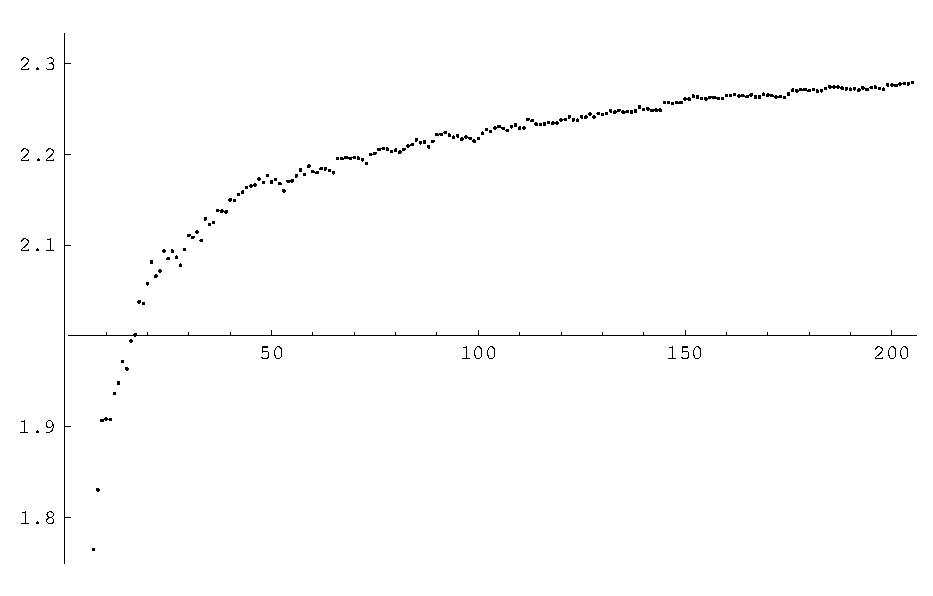
\includegraphics{greedyplot}}
\end{picture}
\caption{The points $\left( k, \log_k(\gamma_k)\right)$ for the greedy Sidon set ${\cal G}_2[2]$.}
\end{figure}


It is interesting to study the greedy sequence with different seeds. Start by setting
$\gamma_1,\dots,\gamma_{r}$, and then continue the sequence in the same manner as above. The resulting sequence
is denoted ${\cal G}_h[g;\gamma_1,\dots,\gamma_r]$.

\begin{cnj}\label{cnj.reciprocals}
For any $h$ and $g$, there are not positive integers $r,\gamma_1,\dots,\gamma_r$ such that
    $$\inf_{\cA \in \Bhg{h}{g}} \left\{ \sum_{a\in\cA} \frac 1a \right\}$$
is achieved with $\cA={\cal G}_h[g;\gamma_1,\dots,\gamma_r]$.
\end{cnj}

This conjecture is dealt with in~\cites{1993.Zhang,2000.Taylor.Yovanof}; it is known that the infimum in
Conjecture~\ref{cnj.reciprocals} (for $g=h=2$) is between $2.16$ and $2.25$.

\subsection{Ruzsa's sets}
A very simple construction of $B_2$ sequences was given by Ruzsa~\cite{1993.Ruzsa}, which is generalized
in~\cite{2004.Martin.OBryant} to $B_2[g^2]$ sequences. Let $\theta$ be a generator of the multiplicative group
modulo the prime $p$. For $k,t\in[p-1]$, let $a_{t,k}$ be the congruence class modulo $p^2-p$ defined by
    \begin{equation*}
    a_{t,k} \equiv t \pmod{p-1} \quad \text{ and } \quad
    a_{t,k} \equiv k \theta^t \pmod{p}.
    \end{equation*}
Define the set
    $$
    \Ruzsa{p}{\theta}{k} := \{a_{t,k} \colon 1\le t < p \} \subseteq \Z/(p^2-p).
    $$
If ${\cal K}$ is any subset of $[p-1]$, then
    $$
    \Ruzsa{p}{\theta}{\cK} := \bigcup_{k\in \cK} \Ruzsa{p}{\theta}{k}
    $$
is a subset of $\Z/(p^2-p)$ with cardinality $|{\cK}|(p-1)$ and
    $$\Ruzsa{p}{\theta}{\cK} \in B_2[|{\cK}|^2].$$

An example is given in Figure~\ref{fig:RuzsaExample}: the row labeled $k$ is $\Ruzsa{13}{2}{k}$. Note that each
row is a translate modulo $13^2-13$ of the row above (and rotated). This is because
    $$a_{t,k\theta}+p\equiv a_{(t+1\bmod{p-1}),k} \pmod{p^2-p},$$
and consequently $\Ruzsa{p}{\theta}{k\theta}+p=\Ruzsa{p}{\theta}{k}$. Since $\theta$ is a generator of the
multiplicative group modulo $p$, this implies that for fixed $p$ and $\theta$ all of the various
$\Ruzsa{p}{\theta}{k}$ are translates of one another.

\begin{figure}\label{fig:RuzsaExample}
    \begin{center}
    $t$\vskip4pt $k$\quad
    \begin{tabular}{|c||cccccccccccc|}\hline
        & 1 & 2 & 3 & 4 & 5 & 6 & 7 & 8 & 9 & 10 & 11 & 12 \\
            \hline \hline
        1&  145& 134& 99& 16& 149& 90& 115& 152& 57& 10& 59& 144  \\
        2&  121& 86& 3& 136& 77&     102& 139& 44& 153& 46& 131& 132 \\
        3&  97& 38& 63& 100& 5& 114& 7& 92& 93&    82& 47& 120 \\
        4&  73& 146& 123& 64& 89& 126& 31&140& 33& 118& 119&    108  \\
        5&  49& 98& 27& 28& 17& 138& 55& 32& 129& 154& 35& 96 \\
        6&  25& 50& 87&    148&101& 150& 79& 80& 69& 34& 107& 84 \\
        7&  1& 2& 147& 112& 29& 6& 103& 128&     9& 70& 23& 72 \\
        8&  133& 110&51& 76& 113& 18& 127& 20& 105& 106& 95&    60 \\
        9&  109& 62& 111& 40& 41& 30& 151& 68& 45& 142& 11& 48 \\
        10&  85&14& 15& 4&     125& 42& 19& 116& 141& 22& 83& 36 \\
        11&  61& 122& 75& 124& 53& 54& 43& 8& 81&     58& 155& 24  \\
        12& 37& 74& 135& 88& 137& 66& 67& 56& 21& 94& 71& 12 \\ \hline
    \end{tabular}
    \caption{Table of $a_{t,k}$ with $p=13$, $\theta=2$. Each row is a Sidon set, the union of any two rows is a
        $\Bhg{2}{8}$ set, the union of any $|\cK|$ rows is a $\Bhg{2}{2|\cK|^2}$ set. Specifically, the row labeled $k$ is
        $\Ruzsa{13}{2}{k}$.}
    \end{center}
\end{figure}

\subsection{Bose's sets}
Bose~\cite{1942.Bose} constructed Sidon sequences by using finite affine geometry. His construction was extended
to $B_h$ sequences (and given in the language of finite fields) in~\cite{1962.Bose.Chowla}, and extended to
$B_2[g^2]$ sequences in~\cite{2004.Martin.OBryant}. Let $q$ be any prime power, $\theta$ a generator of the
multiplicative group of $\GF{q^h}$, and $k \in \GF{q}$, and define the set
    $$
    \Bose{h}{q}{\theta}{k} := \{a \in [q^h-1] \colon \theta^a-k\theta\in \GF{q}\}.
    $$
$\Bose{h}{q}{\theta}{1}$ is $B_h\pmod{q^h-1}$ set, and some work (see~\cite{1945.Bose.Chowla}) has been done on
the question of how quickly these sets can be computed and whether varying $\theta$ (with $h=2$) can help
produce a Sidon set with smaller largest element. If ${\cal K}$ is any subset of $\GF{q}\setminus\{0\}$, then
    $$
    \Bose{2}{q}{\theta}{\cK} := \bigcup_{k\in \cK} \Bose{2}{q}{\theta}{k}
    $$
is a $B_2[|{\cal K}|^2]\pmod{q^2-1}$ sequence.

An example is given in Figure~\ref{fig:BoseExample}, with $q=13$, $h=2$, $\GF{13^2}=\GF{13}[x]/(x^2+2)$, and
$\theta=1+3x$. The column labeled $c_1$ is $\Bose{2}{13}{1+3x\bmod{(13,x^2+2)}}{c_1}$. Note that, as with
Ruzsa's sets, varying $k$ has the effect of translating the set:
    $$\Bose{h}{q}{\theta}{k}=\Bose{h}{q}{\theta}{1}+\log_\theta(k).$$
We note that, unlike Ruzsa's sets, each {\em row} (except the one labeled zero) in Figure~\ref{fig:BoseExample}
is also a Sidon set.


\begin{figure}\label{fig:BoseExample}
    \begin{center}
    $c_1$\vskip4pt $c_0$\quad
    \begin{tabular}{|c||ccccccccccccc|}\hline
         & 0 & 1 & 2 & 3 & 4 & 5 & 6 & 7 & 8 & 9 & 10 & 11 & 12 \\       \hline \hline
        0&  & 77& 147& 21& 49& 35& 91& 7&      119& 133& 105& 63& 161 \\
        1&168& 164& 148& 1& 19& 114& 87& 123&    138& 79&     13& 76& 116 \\
        2&70& 25& 66& 40& 50& 149& 71& 83& 89& 146& 16& 18&     157 \\
        3&112& 23& 58&    108& 125& 31& 92& 20& 67& 113& 60& 82& 131 \\
        4&140&     153& 95& 159& 136& 48& 110& 86& 120& 88& 51& 59&    141 \\
        5&126& 96& 127& 34&     45& 122& 37& 145& 74& 81& 106& 139& 72 \\
        6&14& 90& 93& 137& 128& 15& 10&    130& 27& 152& 101& 33& 162 \\
        7&98& 78& 117& 17& 68& 111& 46& 94& 99& 44&     53& 9& 6 \\
        8&42& 156& 55& 22&    165& 158& 61& 121& 38& 129& 118& 43&     12 \\
        9&56& 57& 143& 135& 4& 36& 2& 26& 132& 52& 75& 11& 69 \\
        10&28&    47& 166&     144& 29& 151& 104& 8& 115& 41& 24& 142& 107 \\
        11&154& 73& 102& 100& 62& 5&     167& 155& 65&    134& 124& 150& 109 \\
        12&84& 32& 160& 97& 163& 54& 39& 3& 30&     103& 85& 64& 80 \\  \hline
    \end{tabular}
    \caption{The least positive integer $k$ such that $(1+3x)^k=c_0 +c_1 x \bmod{(13,x^2+2)}$.
    The column corresponding to $c_1$ is the Sidon set $\Bose{2}{13}{1+3x\bmod{(13,x^2+2)}}{c_1}$.}
    \end{center}
\end{figure}

\subsection{Singer's sets}
Sidon sequences arose incidentally in Singer's work~\cite{1938.Singer} on finite projective geometry. While
Singer's construction gives a slightly thicker Sidon set than Bose's (which is slightly thicker than Ruzsa's),
the construction is more complicated --- even after the simplification of~\cite{1962.Bose.Chowla}. Singer's
construction was extended to $B_2[g^2]$ sequences in~\cite{2004.Martin.OBryant}. No computational work has been
published for Singer's sets.

Let $q$ be any prime power, and let $\theta$ be a generator of the multiplicative group of $\GF{q^{h+1}}$. For
each $\vec{k}=\langle k_1,\dots,k_{h} \rangle \in\GF{q}^{h}$ define the set
    $$
    T(\vec{k} ) := \{0\} \cup \left\{ a \in [q^{h+1}-1] \colon
        \theta^a- \sum_{i=1}^{h} k_i \theta^i \in \GF{q} \right\}.
    $$
Then define
    $$
    \Singer{h}{q}{\theta}{\vec k}
    $$
to be the congruence classes modulo $\frac{q^{h+1}-1}{q-1}$ that intersect $T(\vec k)$. Also define
    $$
    \Singer{h}{q}{\theta}{\cK} := \bigcup_{\vec k\in \cK} \Singer{h}{q}{\theta}{\vec k},
    $$
where $\cK$ is any subset of $\GF{q}^h$. The set $\Singer{h}{q}{\theta}{\langle 1,0,0,\ldots \rangle}$ is a
$B_{h}\pmod{\frac{q^{h+1}-1}{q-1}}$ set. The set $\Singer{2}{q}{\theta}{\langle 1,[k],0 \rangle}$ is a
$\Bhg{2}{2k^2}$ set.




\subsection{Erd\H{o}s \& Tur\`{a}n's sets}
Erd\H{o}s \& Tur\`{a}n~\cite{1941.Erdos.Turan} gave a construction based on quadratic residues. These sets are
substantially thinner than the constructions of Ruzsa, Bose, and Singer given above.

Fix a prime $p$, and let $(k^2)$ be the unique integer in $[p-1]$ congruent to $k^2$ modulo $p$. The set
$\{2pk+(k^2) : 1\leq k <p \}$ is a $B_{2}$ set contained in $[2p+1,2p(p-1)+1]$.

\subsection{Probabilistic Sets}
The seminal paper of Erd\H{o}s \& R\'{e}nyi~\cite{1960.Erdos.Renyi} introducing the probabilistic method to
combinatorial number theory contains a small section on $B_{2}{g}$ sets. The crucial observation made is that
(setting $p_n=1/\sqrt{n}$) the sum
    $$\sum_{n=1}^{N-1} p_n p_{N-n}$$
is bounded independent of $N$. In particular, they prove the existence of an infinite $\Bhg{2}{g}$ set
$a_1<a_2<\cdots$ satisfying
    $$a_k=\bigO{k^{2(1+2/(g-1))}}.$$
See the review of~\cite{1960.Erdos.Renyi} for a more detailed explanation.

See~\cites{1996.3.Kolountzakis, 1998.2.Ruzsa, 1999.Godbole.Janson.Locantore.Rapoport,
2000.Baltz.Schoen.Srivastav, 2001.Ruzsa, Nathanson} for some applications of probability to Sidon sequences, and
vice versa.



\section{The size of finite Sidon sequences}\label{sec.Size}

One of the ``most wanted'' problems is to asymptotically estimate $R_h(g,n)$ for any $h,g$ with $h>2$ or $g>3$.
Also on the ``most wanted'' list is a construction of $\Bhg{h}{g}$ sequences, with $g>h!$, which is dense but is
not merely several $B_h$ sets woven together (such sets do exist:~\cite{1980.Erdos}).

We measure the thickness of $\Bhg{h}{g}$ sets with the quantity:
    $$\sigma_h(g):= \lim_{n\to\infty} \frac{R_h(g,n)}{\sqrt[h]{\floor{g/h!}n}}.$$
Strictly speaking, this limit is not known to exist for $h>2$ or for $g>3$. One should always understand a
lower bound on $\sigma_h(g)$ as being a lower bound on the corresponding $\liminf$, and an upper bound as being
an upper bound on the $\limsup$. If $g=h!$, then we simply write $\sigma_h$.

There are a number of conjectures that are natural to make:
 \begin{enumerate}
    \item   The limit in the definition of $\sigma_h(g)$ is in fact well-defined.
    \item   For each $h$, $\sigma_h(g)$ is an increasing function of $g$.
    \item   For each $h$, $\lim_{g\to\infty} \sigma_h(g)$ is defined and finite.
    \item   If $kh!\le g_1\le g_2 < (k+1)h!$, then $\sigma_h(g_1)=\sigma_h(g_2)$.
 \end{enumerate}
As basic as these questions may seem, they remain unanswered. Regarding question 3, the limit is known to be
bounded between two positive constants. Sadly, there isn't even a conjecture as to growth of $\sigma_h$ as a
function of $h$ (it may well depend on the parity of $h$).

The only explicit values known are $\sigma_2(2)=\sigma_2(3)=1$.

\subsection{$h=2$}
Erd\H{o}s offered USD 500 for answer to the question, ``Is $R_2(2,n)-\sqrt{n}$ unbounded?'' The answer is
likely ``yes''; it is also likely that $R(2,n)-\sqrt{n}$ is nonnegative. Unfortunately, there has been no
progress on these questions since 1941, when it was found that
    $$-n^{\alpha/2} < R(2,n)-\sqrt{n} < n^{1/4}+1,$$
the lower bound holding only for $n$ sufficiently large, with $\alpha$ being a real number such that there is
always a prime between $n-n^{\alpha}$ and $n$ (the current record is $\alpha=0.525$).

\begin{figure}\label{fig:sigma2}
\begin{picture}(432,270)
    \put(0,0){\includegraphics{sigma2g}}
\end{picture}
\caption{The best known upper and lower bounds on $\sigma_2(g)$.}
\end{figure}

The best known upper and lower bounds on $\sigma_2(g)$ are shown in Figure~\ref{fig:sigma2}. The lower bound is
$$
\begin{array}{r@{{}\ge{}}l@{{}>{}}l}
    \sigma_2(4)  & \sqrt{8/7}                   & 1.069, \\ \vspace{1mm}
    \sigma_2(6)  & \sqrt{16/15}                 & 1.032, \\ \vspace{1mm}
    \sigma_2(8)  & \sqrt{8/7}                   & 1.069, \\ \vspace{1mm}
    \sigma_2(10) & \sqrt{49/45}                 & 1.043, \\ \vspace{1mm}
    \sigma_2(12) & \sqrt{6/5}                   & 1.095,
\end{array}
\qquad
\begin{array}{r@{{}\ge{}}l@{{}>{}}l}
    \sigma_2(14) & \sqrt{121/105}               & 1.073, \\ \vspace{1mm}
    \sigma_2(16) & \sqrt{289/240}               & 1.097, \\ \vspace{1mm}
    \sigma_2(18) & \sqrt{32/27}                 & 1.088, \\ \vspace{1mm}
    \sigma_2(20) & \sqrt{40/33}                 & 1.100, \\ \vspace{1mm}
    \sigma_2(22) & \sqrt{324/275}               & 1.085,
\end{array}
$$
and for $g\ge 12$
    $$\sigma_2(2g) \ge \sqrt{2} \frac{g+2\floor{g/3}+\floor{g/6}}{\sqrt{6g^2-2g\floor{g/3}+2g}}.$$
In particular,
    $$\lim_{g\to\infty} \sigma_2(g) \ge \sqrt{121/96} > 1.122.$$
The upper bound is a combination of
    $$\sigma_2(2g) \le \sqrt{\tfrac 74 (2-1/g)}$$
and
$$\frac{\floor{g/2}}{g}\sigma_2(g)^2 \leq
\left\{%
\begin{array}{ll}
    1.74043-{1.00483}/g,
    & \hbox{$g\le8$ and even;} \\
    1.58337-\frac{0.026335}g + \sqrt{0.011572-\frac{0.083397}g+\frac{0.00069356}{g^2}},
    & \hbox{$g\ge 10$ and even;}\\
    1.74043-\frac{4.75492}g,
    & \hbox{$g\le 23$ and odd;} \\
    1.58337-\frac{0.071949}g + \sqrt{0.011572-\frac{0.22784}g+\frac{0.0051768}{g^2}},
    & \hbox{$g\ge 25$ and odd.}
\end{array}%
\right.
$$
In particular,
    $$\lim_{g\to\infty} \sigma_2(g) \le 1.839.$$

For $g=2$, the upper bound is due to Erd\H{o}s \& Tur\`{a}n~\cite{1941.Erdos.Turan} and the upper bound is due to
Singer~\cite{1938.Singer}. For $g=3$, the upper bound is Ruzsa's~\cite{1993.Ruzsa}, and the lower bound is from
$R(g+1,n)\le R(g,n)$. For $g>3$ the upper bound is a combination of Green~\cite{2001.Green} (for small $g$) and
Martin~\& O'Bryant~\cite{Martin.OBryant} (for large $g$). The lower bound for $g=4$ is due to Habsieger \&
Plagne~\cite{2002.Habsieger.Plagne}, the $g=6$ and $g=8$ bounds are due to
\cite{2002.Cilleruelo.Ruzsa.Trujillo}, and for all other even $g$ by Martin \& O'Bryant
\cite{2004.Martin.OBryant}. The lower bounds for odd $g>3$ are just $\sigma_2(2g)\le \sigma_2(2g+1)$.

The proof of $\sigma_2(2) = 1$ is succinct and elegant; we present it momentarily. The upper bound was found
initially in~\cite{1941.Erdos.Turan} and simplified in~\cite{1969.2.Lindstrom}. The lower bound was found in
\cite{1938.Singer} and simplified to this form in~\cite{1993.Ruzsa}.

\begin{thm} The largest Sidon subset of $[n]$ has $\sim \sqrt{n}$ elements, i.e.,
$\sigma_2 = 1$.
\end{thm}

\begin{proof} Let $1\le a_1<a_2< \dots < a_r \le n$ be a Sidon sequence, and
consider the differences (the parameter $u$ will be set to $\floor{n^{1/4}}$):
    \begin{center}
    $a_2-a_1, \quad a_3-a_2,\quad \dots,\quad a_r-a_{r-1}$ \\
    $a_3-a_1, \quad a_4-a_2,\quad  \dots, \quad a_r-a_{r-2}$ \\
    $\vdots$ \\
    $a_{u+1}-a_1, \quad a_{u+2}-a_2,\quad  \dots,\quad a_r-a_{r-u}$
    \end{center}
The $k$-th row contains $r-k$ differences, and since $\{a_i\}$ is a Sidon set, these differences are distinct.
That's a total of $\sum_{i=1}^u (r-i) = ru-\frac12 u(u+1)$ differences. The sum of all these differences is at
least
    $$\sum_{i=1}^{ru-u(u+1)/2} i = \frac12\left(ru-\tfrac12 u(u+1)\right)\left(ru-\tfrac12 u(u+1)+1\right).$$
On the other hand, the sum of the differences in the $k$-th row telescopes to
    $$\sum_{i=r-k+1}^r a_i - \sum_{i=1}^k a_i < kn, $$
and so the sum of all the differences is less than $\sum_{k=1}^u kn=nu(u+1)/2$. Comparing the upper and lower
bounds yields an inequality in terms of $n$, $r$, and $u=\floor{n^{1/4}}$. Calculus implies that
$r<n^{1/2}+n^{1/4}+1$, which in turn implies that $\sigma_2 \le 1$.

We now give Ruzsa's construction of a Sidon set contained in $p(p-1)$ with $p-1$ elements ($p$ is any odd
prime), from which it follows (using the elementary fact that the ratio between consecutive primes goes to 1)
that $\sigma_2 \ge 1$. Let $\theta$ be a primitive root modulo $p$, and consider the set $\cA$ of integers
$a_t$ ($1\le t < p-1$) defined by
    $$1\le a_t < p^2-p \quad \text{ and } \quad
    a_t \equiv t \pmod{p-1} \quad\text{ and } \quad
    a_t \equiv \theta^t \pmod{p}.$$
Now suppose, by way of contradiction, that there are three pairs $(a_{r_m},a_{v_m})\in \cA \times \cA$
satisfying $a_{r_m}+a_{v_m}= k $ (for some fixed $k\in\Z$). Each pair gives rise to a factorization modulo $p$
of
    $$x^2 - k x + \theta^k\equiv (x-a_{r_m})(x-a_{v_m}) \pmod{p},$$
using the critical relation $a_{r_m}a_{v_m}\equiv \theta^{r_m+v_m}=\theta^k \pmod{p}$. Factorization modulo $p$
is unique, so it must be that two of the three pairs are congruent modulo $p$, say
    \begin{equation}\label{modp:eq}
    a_{r_1}\equiv a_{r_2} \pmod{p}.
    \end{equation}
In this case, $\theta^{r_1} \equiv a_{r_1}\equiv a_{r_2} \equiv \theta^{r_2} \pmod{p}$. Since $\theta$ has
multiplicative order $p-1$, this tells us that $r_1 \equiv r_2 \pmod{p-1}$. Since $a_{r_m} \equiv r_m
\pmod{p-1}$ by definition, we have
    \begin{equation}\label{modp-1:eq}
    a_{r_1} \equiv a_{r_2} \pmod{p-1}.
    \end{equation}
Equations \eqref{modp:eq} and \eqref{modp-1:eq}, together with $a_{r_1}+a_{v_1} = k = a_{r_2}+a_{v_2}$ imply
that the pairs $(a_{r_1},a_{v_1}), (a_{r_2},a_{v_2})$ are identical, and so there are {\em not} three such
pairs. Thus, $\cA$ is a Sidon set. In particular, $\cA=\Ruzsa{p}{\theta}{1}$.
\end{proof}

A Sidon sequence $a_1<a_2<\dots<a_k$ is called ``short'' if $a_k-a_1$ is as small as possible.
Figure~\ref{fig:SidonSets} contains (up to reflection and translation) all of the short Sidon sequences with
$k\le 10$, and two of the short Sidon sequences with $k=11$; I don't know if there are more. It is rumored that
Imre Ruzsa has computed that $\min\{a_{12}-a_1\} = 85$, $\min\{a_{13}-a_1\}= 106$, $\min\{a_{14}-a_1\}=127$. It
is likely that for each $k$, there is short Sidon set with $a_1=0$ and $a_2=1$, while it seems likely that each
triple $(a_1,a_2,a_3)$ is the beginning of only finitely many short Sidon sequences.


\begin{figure}\label{fig:SidonSets}
    \begin{center}
        \begin{tabular}{ccc}
        $k$  & $\min\{a_k-a_1\}$ &             Witness              \\
        \hline
        2  &        1        &             \{0,1\}              \\
        3  &        3        &            \{0,1,3\}             \\
        4  &        6        &           \{0,1,4,6\}            \\
        5  &       11        &          \{0,1,4,9,11\}          \\
        &                 &          \{0,2,7,8,11\}          \\
        6  &       17        &       \{0,1,4,10,12,17\}         \\
        &                 &       \{0,1,4,10,15,17\}         \\
        &                 &       \{0,1,8,11,13,17\}         \\
        &                 &       \{0,1,8,12,14,17\}         \\
        7  &       25        &      \{0,1,4,10,18,23,25\}       \\
        &                 &      \{0,1,7,11,20,23,25\}       \\
        &                 &      \{0,1,11,16,19,23,25\}      \\
        &                 &      \{0,2,3,10,16,21,25\}       \\
        &                 &      \{0,2,7,13,21,22,25\}       \\
        8  &       34        &     \{0,1,4,9,15,22,32,34\}      \\
        9  &       44        &   \{0,1,5,12,25,27,35,41,44\}    \\
        10 &       55        &  \{0,1,6,10,23,26,34,41,53,55\}  \\
        11 &       72        & \{0,1,4,13,28,33,47,54,64,70,72\} \\
        &                 &  \{0,1,9,19,24,31,52,56,58,69,72\}  \\
        \end{tabular}
    \caption{Shortest Sidon sequences (from~\cite{2004.Martin.OBryant})}
    \end{center}
\end{figure}

Figure~\ref{fig:R(g,n)} gives the values of $n$ for which $R(g,n)-R(g,n-1)=1$. This table was computed using the
easiest algorithm and a small amount of time. I encourage the interested reader (or her students!) to extend it.

The construction given in~\cite{2002.Cilleruelo.Ruzsa.Trujillo} is optimized by choosing $x$ so that
$R(g,x)/\sqrt{gx}$ is maximized. This appears to happen (for each $g$) with a fairly small value of $x$; a
formula would lay to rest further optimization efforts (such as those in
\cites{2002.Habsieger.Plagne,2004.Martin.OBryant}). Even given a perfect optimization, however, it is unlikely
that this construction is optimal in any sense.

\begin{figure}\label{fig:R(g,n)}
\small
\begin{center}
$g$\vskip4pt $k$\quad
\begin{tabular}{|c||r|r|r|r|r|r|r|r|r|r|}
\hline
    &          2 &          3 &         4 &         5 &         6 & 7 & 8 & 9 &    10     &    11     \\ \hline\hline
 3  &          4 &            &           &           &           & & & & &           \\ \hline
 4  &          7 &          5 &           &           &           & & & & &           \\ \hline
 5  &         12 &          8 &         6 &           &           & & & & &           \\ \hline
 6  &         18 &         13 &         8 &         7 &           & & & & &           \\ \hline
 7  &         26 &         19 &        11 &         9 &         8 & & & & &           \\ \hline
 8  &         35 &         25 &        14 &        12 &        10 & 9 & & & &           \\ \hline
 9  &         45 &         35 &        18 &        15 &        12 & 11 & 10 &           &           &           \\ \hline
 10 &         56 &         46 &        22 &        19 &        14 & 13 & 12 &        11 &           &           \\ \hline
 11 &         73 &         58 &        27 &        24 &        17 & 15 & 14 &        13 &    12     &           \\ \hline
 12 &  $\leq 92$ &  $\leq 72$ &        31 &        29 &        20 & 18 & 16 &        15 &    14     &        13 \\ \hline
 13 & $\leq 123$ & $\leq 101$ &        37 &        34 &        24 & 21 & 18 &        17 &    16     &        15 \\ \hline
 14 & $\leq 140$ & $\leq 128$ &        44 &        40 &        28 & 26 & 21 &        19 &    18     &        17 \\ \hline
 15 & $\leq 163$ &            & $\leq 52$ & $\leq 47$ &        32 & 29 & 24 &        22 &    20     &        19 \\ \hline
 16 & $\leq 195$ &            &           &           &        36 & 34 & 27 &        24 &    22     &        21 \\ \hline
 17 &            &            &           &           & $\leq 42$ & $\leq 38$ &        30 &        28 &    24     &        23 \\ \hline
 18 &            &            &           &           &           & & 34 & 32 &    27     &        25 \\ \hline
 19 &            &            &           &           &           & & $\leq 38$ & $\leq 36$ &    30     &        28 \\ \hline
 20 &            &            &           &           &           & & & & 33     &        31 \\ \hline
 21 &            &            &           &           &           & & & & $\leq 37$ &        35 \\ \hline
 21 &            &            &           &           &           & & & & & $\leq 38$ \\ \hline
\end{tabular}
\caption{$\min\{n\colon R_2(g,n) \geq k\}$ (from~\cite{2004.Martin.OBryant}, extended by John Trono)}
\end{center}\end{figure}

\subsection{$h>2$}

\begin{figure}\label{fig:sigmah}
\begin{picture}(436,280)
    \put(428,11){$h$}
    \put(24,272){$\sigma_h$}
    \put(0,0){\includegraphics{sigmah}}
\end{picture}
\caption{The best known upper and lower bounds on $\sigma_h$.}
\end{figure}

Very little is understood about $B_h$ sets for $h>2$. The construction of Bose \& Chowla~\cite{1962.Bose.Chowla}
show that $\sigma_h\ge 1$, and we know that $\sigma_2=1$. Various improvements on the upper bound on $\sigma_h$
were given in~\cites{1961.Kruckeberg, 1969.3.Lindstrom, 1984.Dyachkov.Rykov, 1986.Shparlinski, 1993.Jia,
1994.Chen, 1996.1.Kolountzakis}

Cilleruelo~\cite{2001.Cilleruelo} proved that $\sigma_3 \le 1.576$, $\sigma_4 \le 1.673$, and for $h>75$,
    $$\sigma_h^h \le \frac 52 \left(\tfrac{15}{4}-\tfrac{5}{4\ceiling{h/2}}\right)^{1/4}
    \frac{(\ceiling{h/2}!)^2}{\sqrt{\ceiling{h/2}}} $$
for odd $h$, and
    $$\sigma_h^h \le \frac 52 \left(\tfrac{15}{4}-\tfrac{5}{2h}\right)^{1/4}
    ((h/2)!)^2 \sqrt{h/2}$$
for even $h$. He does give improvements for $h\in[5,74]$ also.

Ben Green~\cite{2001.Green} has improved these upper bounds and shown
    \begin{align*}
    \sigma_3 &\le (7/2)^{1/3} < 1.519 \\
    \sigma_4 &\le 7^{1/4} < 1.627  \\
    \sigma_h &\le \frac{1}{2e}\left( h + \frac32 \log h + o_h(\log h)\right).
    \end{align*}
Green's bound for $\sigma_h$ ultimately relies on the observation that if $X_i$ are independent random variables
taking values uniformly in a set of integers $\cA$, then the central limit theorem implies that
$X_1+X_2+\dots+X_h$ has a normal distribution (for large $h$). While Green's bound is not given in an effective
form, we presume that this could be done in a straightforward manner.

\subsection{Cyclic groups}

The earliest appearances of Sidon sets were as Monthly problems~\cites{1906.Veblen, 1906.Dickson} asking for
Sidon subsets of $\Z_n$. If $\cA$ is a $\Bhg{h}{g}(\bmod{ m})$ set and $\gcd(k,m)=1$, then so is $k \cA+r=\{ka+r
\colon a\in \cA\}$; we say that $\cA$ and $k\cA+r$ are equivalent. Veblen and Dickson asked for all inequivalent
Sidon subsets of $\Z_n$ for various $n$. The number of inequivalent modular Sidon sets that arise from the
construction of Bose \& Chowla is investigated in~\cites{1963.Halberstam.Laxton,1964.Halberstam.Laxton}.

The constructions of Ruzsa, Bose, and Singer all give {\em modular} Sidon sets. This would seem to be a more
symmetric setting, and so an easier setting. Unfortunately, while the constructions are naturally modular, the
upper bounds on $R_h(g,n)$ sets all seem to fundamentally rely on the {\em asymmetry} of $[n]$. Progress (beyond
the very little in~\cite{2004.Martin.OBryant}) on bounding $C_h(g,n)$ would be a significant contribution.
Here's what is known about $C_2(g,n)$:

\begin{thm} \label{C.upperbound}
    Let $q$ be a prime power, and let $k, g,f,x,y$ be positive integers with $k<q$.
    \renewcommand{\theenumi}{\roman{enumi}}
    \begin{enumerate}
    \item   $\binom{C_2(2,n)}{2} \le \floor{\frac n2}$, and in particular $C_2(2,n)\le \sqrt{n}+1$;
    \item   $C_2(3,n) \le \sqrt{n+9/2}+3$;
    \item   $C_2(4,n) \le \sqrt{3n} + 7/6$;
    \item   $C_2(g,n) \le \sqrt{gn}$ for even $g$;
    \item   $C_2(g,n) \le \sqrt{1-\tfrac1g}\sqrt{gn}+1$, for odd $g$.
    \item If $q$ is a prime, then $C_2(2k^2,q^2-q)) \geq k (q-1)$;
    \item $C_2(2k^2,q^2-1) \geq k q$;
    \item $C_2(2k^2,q^2+q+1) \geq kq+1$;
    \item If $\gcd(x,y)=1$, then $C_2(gf,xy)\geq C_2(g,x)C_2(f,y)$;
    \end{enumerate}
\end{thm}

\section{The size of infinite Sidon sequences}\label{sec.Size2}

Let $\cA\subseteq \Z$ be a Sidon sequence, and let $A(n)=\#(\cA \cap [n])$. St\"{o}hr~\cite{1955.Stohr} strengthens
an unpublished result of Erd\H{o}s and proved that
    $$\liminf_{n\to\infty} \frac{A(n)}{\sqrt{n/\log(n)}}\not=\infty$$
St\"{o}hr also gave Erd\H{o}s's proof that there is a Sidon sequence with
    $$\limsup_{n\to\infty} \frac{A(n)}{\sqrt{n}} \ge \frac 12;$$
this was improved by Kr\"{u}ckeberg~\cite{1961.Kruckeberg} to $1/\sqrt{2}$, and taken to $\Bhg{2}{g}$ sequences by
Cilleruelo \& Trujillo~\cite{2001.Cilleruelo.Trujillo}. In~\cite{1981.Ajtai.Komlos.Szemeredi} a Sidon sequence
is constructed with
    $$A(n)> 10^{-3} (n \log n)^{1/3}$$
for sufficiently large $n$. Erd\H{o}s asked~\cite{1982.Erdos} if there is a sequence $a_1<a_2<\dots$ with $a_k =
\littleo{k^{3-\epsilon}}$ for any positive $\epsilon$; Ruzsa constructed a Sidon sequence with $A(n)\sim
n^{\sqrt{2}-1+\littleo{1}}$.

Sheng Chen~\cite{1993.Chen} conjectures that if $\cA$ is a $B_{h}$ sequence with counting function $A(n)$, then
    $$\liminf_{n\to\infty} A(n) \left(\tfrac{\log n}{n}\right)^{1/h}$$
is finite. See also~\cites{1994.Helm, 1994.Jia, 1993.1.Helm, 1993.2.Helm, 1989.Nash, 1989.Jia, 1996.Chen,
1996.Helm, MR97d:11040}. Neither the results nor the conjectures have been extended to $\Bhg{h}{g}$ sequences.


\section{The distribution of $\cA$ and $\cA+\cA$}\label{sec.distribution}

If $\cA_n\subset [n]$ is a sequence of Sidon sets and $|\cA| \sim \sqrt{n}$, then $\cA_n$ becomes uniformly
distributed in $[n]$ (see~\cite{1991.Erdos.Freud}). Moreover, $\cA_n$ becomes uniformly distributed in
congruence classes modulo $m$ (for any fixed $m$) (see~\cites{1998.2.Lindstrom, 1999.Kolountzakis,
2002.Schoen}). It is shown in~\cite{1994.2.Erdos.Sarkozy.Sos} that if $\cA$ is any finite Sidon sequence, then
the sumset $\cA+\cA$ consists of at least $c|\cA|^2$ intervals (for an unspecified constant $c$). With care this
can be improved to $(|\cA|^2-|\cA|-1)/4$. Extensive computations indicate that if $|\cA| \sim \sqrt{n}$, then
$\cA+\cA$ consists of $\sim |\cA|^2/3$ intervals. Very little is known about the structure of $\cA+\cA$. Must
the size of the longest interval in $\cA+\cA$ go to infinity as $n$ does (with $|\cA|\sim\sqrt{n}$)?

Martin \& O'Bryant~\cite{Martin.OBryant} conjecture that $\Bhg{2}{g}$ sets with maximal size are uniformly
distributed. Current computations are insufficient to extend this conjecture to $\Bhg{h}{g}$ sets.



\section{Restricted Sidon sequences}\label{sec.SpecialSequences}

A well known conjecture~\cite{1994.Guy} states that the fifth powers $0, 1, 32, 243,\dots$ are a Sidon sequence.
Ruzsa~\cite{2001.Ruzsa} shows that there is an $\alpha$ such that $\{n^5+\floor{\alpha n^4}\colon n\ge n_0\}$ is
a Sidon set. Cilleruelo~\cite{1995.Cilleruelo} considered Sidon sequences all of whose terms are squares. Abbot
\cite{1990.Abbott} studied the size of Sidon sequences contained in an arbitrary set of integers with
cardinality $n$ (there is one with size at least $\frac 2{25} \sqrt{n}$).

Lindstr\"{o}m~\cites{1969.1.Lindstrom,1972.Lindstrom} initiated the study of $\Bhg{h}{g}$ sets in group $\Z^d$.

Erd\H{o}s~\cite{1980.Erdos} investigated Sidon subsets of $\Bhg{2}{g}$ sets. Alon \& Erd\H{o}s
\cite{1985.Alon.Erdos} considered the problem of decomposing a finite $\Bhg{2}{g}$ into $B_2$ sets; how many
$B_2$ sets are needed?

\section{Generalizations}

The graph theorist's analogs of Sidon sets are magic and harmonious labelings. See
\cites{1980.1.Graham.Sloane,1980.2.Graham.Sloane}.

The bigger setting for the Sidon question is that of sets which avoid a linear form. Let $L$ be an $m\times n$
matrix of integers. The set $\cA$ is said to avoid $L$ if there are no nontrivial solutions to
$L\vec{a}=\vec{0}$ with $\vec{a}=(a_1,a_2, \dots ,a_n)^T, a_k\in \cA$. Sidon sets are the special case
$L=[1,1,-1,-1]$, sets with 3-term arithmetic progressions are the case $L=[1,-2,1]$, etc. It is surprising that
in such a general setting significant and strong results can be found. Precisely this is done
in~\cites{1972.Komlos.Sulyok.Szemeredi, 1975.Komlos.Sulyok.Szemeredi,1993.Ruzsa}.

\section{Other open questions}\label{sec.OpenQuestions}

If $\cA^\ast$ is bounded, is it necessarily 0 infinitely often? This is equivalent to a USD 500 question of
Erd\H{o}s~\cite{1989.Erdos}: If every positive integer can be written as a sum of two elements of
$\cB\subseteq\N$ (i.e., $\cB$ is a base), must the number of ways to do so go to infinity?

Is there an anti-Freiman theorem: If $|\cA+\cA|/|\cA|^2 > c$, then $\cA$ has a large $\Bhg{2}{g}$ subset, where
$g$ and `large' depend only $c$? This question may be related to the quasi-Sidon sets discussed
in~\cites{1991.Erdos.Freud, Pikhurko}.



\section{Bibliography}



\begin{biblist}
%---------------------------------------------------------------------------------------
\bib{1906.Veblen}{article}{
    author={Veblen, Oswald},
     title={\href{http://links.jstor.org/sici?sici=0002-9890\%28190602\%2913\%3A2\%3C46\%3ADA1\%3E2.0.CO\%3B2-A}
            {Diophantine analysis: problem 132}},
      date={Feb 1906},
   journal={Amer. Math. Monthly},
    volume={13},
    number={2},
     pages={46},
      note={\href{http://links.jstor.org/sici?sici=0002-9890\%28190611\%2913\%3A11\%3C215\%3A1\%3E2.0.CO\%3B2-K}
            {Solution} by F. H. Safford appears in {\bf 13} (Nov 1906), 215.},
}

\annotation{The problem reads: ``From the numbers, $0, 1, 2,\dots$, 42, select seven, such that the 42
differences of these seven numbers shall be congruent $\pmod{43}$ to the numbers $0, 1, 2, \dots, 42$.
The differences may be both $+$ and $-$.''

The solution concludes: ``Hence the problem is impossible.''}


%---------------------------------------------------------------------------------------
\bib{1906.Dickson}{article}{
    author={Dickson, L.~E.},
     title={\href{http://links.jstor.org/sici?sici=0002-9890\%28190611\%2913\%3A11\%3C219\%3ADA1\%3E2.0.CO\%3B2-X}
            {Diophantine analysis: Problem 142}},
      date={Nov 1906},
   journal={Amer. Math. Monthly},
    volume={13},
    number={11},
     pages={219},
      note={\href{http://links.jstor.org/sici?sici=0002-9890\%28190705\%2914\%3A5\%3C107\%3A1\%3E2.0.CO\%3B2-D}
      {Solution} by L. E. Dickson appears in {\bf 14} (May 1907):107 \ndash 108.},
}

\annotation{The problem reads: ``Let $n$ be an integer $>1$ and set $p=n(n-1)+1$. Required $n$ integers
whose $n(n-1)$ differences are congruent (modulo $p$) to the numbers $1, 2, \dots,p-1$. Exhibit at least
for $n=3,4,5$, all inequivalent sets of solutions where a set $a_1,a_2, \dots, a_n$ is called equivalent
to the $m(a_1-d),m(a_2-d),\dots, m(a_n-d)$, for any integers $m$ and $d$ ($m$ not divisible by $p$).''

For $n=3,4,5,6,8$ there is a unique set, and for $n=7$ there are none. The solutions are $n=3
\Rightarrow \{0,1,3\}$, $n=4 \Rightarrow \{0,1,3,9\}$, $n=5 \Rightarrow \{0,1,6,8,18\}$, $n=6
\Rightarrow \{0,1,3,10,14,26\}$, and $n=8 \Rightarrow \{0,1,3,13,32,36,43,52\}$.}

%---------------------------------------------------------------------------------------
\bib{1932.Sidon}{article}{
    author={Sidon, S.},
     title={Ein Satz \"{u}ber trigonomietrische Polynome und seine Anwendungen in der Theorie der Fourier-Reihen},
      date={1932},
   journal={Math. Annalen},
    volume={106},
     pages={536\ndash 539},
}


%---------------------------------------------------------------------------------------
\bib{1938.Singer}{article}{
    author={Singer, James},
     title={A theorem in finite projective geometry and some applications to number theory},
      date={1938},
      ISSN={0002-9947},
   journal={Trans. Amer. Math. Soc.},
    volume={43},
    number={3},
     pages={377\ndash 385},
    review={\MR{1501951}},
}

\annotation{Using finite projective geometry, Singer shows that for $p$ a prime power, $C_2(2,p^2+p+1)\geq
p+1$. An algebraic outline of his argument follows. Let $\theta\in \GF{p^3}$ be a primitive element. Then
$\{1,\theta,\theta^2\}$ is a basis of $\GF{p^3}$ over $\GF{p}$, hence for each $a\in\Z$, there are unique
$r_a,m_a,n_a\in \GF{p}$ such that $\theta^a=r_a \theta^2+m_a\theta+n_a$. The set $\{0\} \cup \{a \in [0,p^3-1)
\colon (r_a,m_a)=(0,1)\}$, reduced modulo $p^2+p+1$, witnesses $C_2(2,p^2+p+1)\geq p+1$.}

\articlecites{\cite{1906.Veblen},~\cite{1906.Dickson}}

%---------------------------------------------------------------------------------------
\bib{1941.Erdos.Turan}{article}{
    author={Erd\"{o}s, P.},
    author={Tur\`{a}n, P.},
     title={On a problem of Sidon in additive number theory, and on some related problems},
      date={1941},
   journal={J. London Math. Soc.},
    volume={16},
     pages={212\ndash 215},
    review={\MR{3,270e}},
}

\annotation{The authors demonstrate that $\forall \epsilon>0 \,\exists n_0$ such that
$(\frac{1}{\sqrt{2}}-\epsilon)\sqrt{n} < R_2(2,n) < \sqrt{n}+\bigO{n^{1/4}}$ for all $n>n_0$.

The lower bound comes from $R_2(2,2p^2)\geq p-1$ ($p$ prime), which is witnessed by $\{2pk+(k^2) \colon 1\leq k
<p \}$, where $(k^2)$ is the unique integer in $[1,p)$ congruent to $k^2$ modulo $p$.

The upper bound (the argument can actually be made to give $R_2(2,n)<n^{1/2}+n^{1/4}+1$) is repeated almost
verbatim as Theorem 4 in~\cite{1983.Halberstam.Roth}*{Chapter II}. Let $S\subset[n]$ be a Sidon set with maximal
cardinality, and let $A_u=|S\cap[-n^{3/4}+u,u)|$. The idea is to bound $\sum \binom{A_u}{2}$ above and below.
The lower bound uses Cauchy's inequality, and the upper bound uses the observation that $(s_i,s_j)\in S\times S$
is determined by $s_i-s_j$, i.e., Sidon sets not only have distinct sums, but distinct differences as well.}

\articlecites{\cite{1932.Sidon}}

%---------------------------------------------------------------------------------------
\bib{1942.Bose}{article}{
    author={Bose, R.~C.},
     title={An affine analogue of Singer's theorem},
      date={1942},
   journal={J. Indian Math. Soc. (N.S.)},
    volume={6},
     pages={1\ndash 15},
    review={\MR{4,33c}},
}

\annotation{Using finite affine geometry, Bose demonstrates that for $p$ a prime power, $C_2(2,p^2-1)\geq p$.
This theorem is only slightly weaker (in terms of $\frac{C_2(g,n)}{\sqrt{gn}}$) than Singer's
\cite{1938.Singer}, while his proof is substantially simpler. His argument, in algebraic form, is as follows.
Let $\theta \in \GF{p^2}$ be a primitive element. For each $a\in\Z$, there is a unique $m_a,n_a \in \GF{p}$
such that $\theta^a=m_a \theta+n_a$. The set $\{a\in[0,p^2-1) : m_a=1\}$ witnesses $C_2(2,p^2-1)\geq p$.}

\articlecites{\cite{1938.Singer}}

%---------------------------------------------------------------------------------------
\bib{1944.Chowla}{article}{
    author={Chowla, S.},
     title={Solution of a problem of Erd\"os and Turan in additive-number  theory},
      date={1944},
   journal={Proc. Nat. Acad. Sci. India. Sect. A.},
    volume={14},
     pages={1\ndash 2},
    review={\MR{7,243b}},
}

\annotation{Chowla notes that the constructions of Bose~\cite{1942.Bose} or of Singer~\cite{1938.Singer} may be
combined with the bound of Erd\"{o}s \& Tur\`{a}n~\cite{1941.Erdos.Turan} to give $R_2(2,n)\sim \sqrt{n}$, i.e.,
$\sigma_2=1$. Chowla also notes that $R_2(2,n)\geq C_2(2,n-1)+1$ by adjoining $n$ to any subset of $[n-1]$ which
is a $B_2\pmod{n-1}$ set and contains 1. Chowla also points out that the error term in the lower bound of
$R_2(2,n)$ depends on a result of the form ``For sufficiently large $n$ there is a prime between $n$ and
$n-n^\theta$.''}

\articlecites{\cite{1941.Erdos.Turan},~\cite{1942.Bose}}

%---------------------------------------------------------------------------------------
\bib{1944.2.Chowla}{article}{
    author={Chowla, S.},
     title={Solution of a problem of Erd\"os and Turan in
            additive-number-theory},
   journal={Proc. Lahore Philos. Soc.},
    volume={6},
      date={1944},
     pages={13\ndash 14},
    review={\MR{7,243c}},
}

%---------------------------------------------------------------------------------------
\bib{1944.Erdos}{article}{
    author={Erd\"{o}s, P.},
     title={On a problem of Sidon in additive number theory and on some related
  problems. Addendum},
      date={1944},
   journal={J. London Math. Soc.},
    volume={19},
     pages={208},
    review={\MR{7,242f}},
}

\annotation{Erd\H{o}s observes that~\cite{1938.Singer} and~\cite{1941.Erdos.Turan} together imply $R_2(2,n)\sim
\sqrt{n}$, i.e., $\sigma_2=1$.}

\articlecites{\cite{1938.Singer},~\cite{1941.Erdos.Turan}}

%---------------------------------------------------------------------------------------
\bib{1944.Chowla.Mian}{article}{
    author={Mian, Abdul~Majid},
    author={Chowla, S.},
     title={On the $B\sb 2$ sequences of Sidon},
      date={1944},
   journal={Proc. Nat. Acad. Sci. India. Sect. A.},
    volume={14},
     pages={3\ndash 4},
    review={\MR{7,243a}},
}

\annotation{Nothing is proved here, but the first 11 terms of the greedy Sidon set are reported, and it is
noted that this supports the conjecture that $R_2(2,n)\geq \sqrt{n}$ for all $n$.

The greedy Sidon set begins $a_1=1, 2, 4, 8, 13, 21, 31, 45, 66, 81, 97,\dots$. The authors state ``It seems
likely that $$\lim_{m\to\infty} \frac{a_{m+1}-a_m}{m} =2$$ as far as our table goes, we have $\sqrt{a_m} \leq
m$.'' However, $a_{17}=290>17^2$.}

\articlecites{\cite{1932.Sidon},~\cite{1941.Erdos.Turan}}

%---------------------------------------------------------------------------------------
\bib{1945.Bose.Chowla}{article}{
    author={Bose, R.~C.},
    author={Chowla, S.},
     title={On the construction of affine difference sets},
      date={1945},
   journal={Bull. Calcutta Math. Soc.},
    volume={37},
     pages={107\ndash 112},
    review={\MR{7,365g}},
}

\annotation{This paper considers of the mechanics of converting Bose's construction~\cite{1942.Bose} into actual
numbers. Suppose that $p$ is a power of a prime, and $\theta\in \GF{p^2}$ is a primitive element satisfying
$\theta^2+a\theta+b=0$. Define $f_1=0$ and $f_m\equiv \tfrac{b}{a-f_m} \pmod{p}$. Define also $\log_b(N)$ to be
the unique integer $t\in [0,p)$ such that $b^t \equiv N \pmod{p}$. Then the set $\{d_1,\dots,d_p\}$, defined by
$d_1=1, d_{m-1}=1+d_m-(p+1) \ind(f_m-a)$, witnesses $C_2(2,p^2-1)\geq p$.}

\articlecites{\cite{1938.Singer}}

%---------------------------------------------------------------------------------------
\bib{1955.Stohr}{article}{
    author={St\"{o}hr, Alfred},
     title={Gel\"oste und ungel\"oste Fragen \"uber Basen der nat\"urlichen Zahlenreihe. I, II},
      date={1955},
   journal={J. Reine Angew. Math.},
    volume={194},
     pages={40\ndash 65, 111\ndash 140},
    review={\MR{17,713a}},
}

\annotation{This survey addresses Sidon sets in $\S 12 a\beta$ on pages 129--135. Two results of Erd\H{o}s
are given: There is an infinite Sidon set whose counting function $A(n)$ satisfies $\limsup
\frac{A(n)}{\sqrt{n}} \geq \frac12$; Every infinite Sidon set has a counting function $A(n)$ satisfying
$\liminf \frac{A(n)}{\sqrt{n}}=0$.

St\"{o}hr notes that this second result shows that the guess of Mian \& Chowla~\cite{1944.Chowla.Mian} that the
$n$-th term of the greedy Sidon set is at most $n^2$ is false. He also notes that the second statement (and its
proof) can be made more precise: Every infinite Sidon set has a counting function $A(n)$ satisfying $\liminf
\frac{A(n)\sqrt{\log n } }{\sqrt{n}} \ll 1$. These results are also reported as Theorems 8 and 9 of
\cite{1983.Halberstam.Roth}*{Chapter II}.

St\"{o}hr then raises the question of how large $\liminf \frac{A(n)\sqrt{\log n } }{\sqrt{n}}$ can be, and
if the answer is 0, then what would be a suitable replacement for $\frac{\sqrt{\log n}}{\sqrt{n}}$. He
also asks if there is a Sidon set for which $0< \liminf \frac{A(n)\sqrt{\log n } }{\sqrt{n}}\leq \limsup
\frac{A(n)\sqrt{\log n } }{\sqrt{n}}<\infty$. Similar questions are raised for $B_h$ sets.

St\"{o}hr then considers the greedy Sidon set, and notes that its $n$-th element $a_n$ is at most $(n-1)^3+1$.}

\articlecites{\cite{1938.Singer},~\cite{1941.Erdos.Turan},~\cite{1944.Chowla},~\cite{1944.Erdos},
\cite{1944.Chowla.Mian}}

%---------------------------------------------------------------------------------------
\bib{1960.Erdos.Renyi}{article}{
    author={Erd{\H{o}}s, P.},
    author={R\'{e}nyi, A.},
     title={Additive properties of random sequences of positive integers},
      date={1960},
   journal={Acta Arith.},
    volume={6},
     pages={83\ndash 110},
    review={\MR{22:10970}},
}

\annotation{This papers examines the behavior of $S^\ast(n)$ for sets $S$ defined by $\Prob(k\in S)=p_k$, for
various sequences $p_k$. The result relating to Sidon sequences states that for every $\delta>0$, there exists
a $B^\ast[g]$ sequence $\{a_1,a_2,\dots\}$ satisfying $a_k=\bigO{k^{2(1+2(g-1)^{-1})}}$.

We give the main steps of the proof. Set $p_n=n^{-\frac12-\epsilon}$ (with $\epsilon > (g+1)^{-1}$) and
$q_n=1-p_n$. Define the independent random variables $X_n$ to be 1 with probability $p_n$ and 0 with
probability $q_n$. Define the random function $f(n)=\sum_{k=1}^{n/2} X_kX_{n-k}$; we wish to show that
almost surely $f(n) \leq \frac{g}{2}$ (with finitely many exceptions). Then
 \begin{align*}
    \E[\exp(t f(n) )] &=\prod_{k\leq n/2} \left(1+
        \frac{e^t-1}{(k(n-k))^{1/2+\epsilon}}\right) \\
                    & \leq \prod_{k \leq n/2} \exp \left(
                        \frac{e^t-1}{(k(n-k))^{1/2+\epsilon}}\right) \\
                    &\leq
                        \exp\left(\frac{e^t-1}{n^{2\epsilon}}I(\epsilon)\right),
 \end{align*}
where $I(\epsilon)$ is a constant depending only on $\epsilon$ as $n\to\infty$. Set
$t=\log(1+n^{2\epsilon})$ and apply the Exponential Chebyshev Theorem to find (with $K=g/2$):
    $$\Prob(f(n) > K) \leq \frac{\E[\exp(t f(n))]}{\exp(t(K+1))} \leq \frac{C_1}{n^{2\epsilon(K+1)}}.$$
Thus $\sum_{n=1}^\infty P(f(n) > K)$ converges, and the Borel-Cantelli Lemma guarantees that $\{n \colon
X_n=1\}$ is almost surely a $B^\ast[g]$ sequence (at least, after deleting finitely many terms).

This, and other results of this paper, are given in~\cite{1983.Halberstam.Roth}*{Chapter 3}.}

\articlecites{\cite{1932.Sidon},~\cite{1941.Erdos.Turan}}

%---------------------------------------------------------------------------------------
\bib{1961.Kruckeberg}{article}{
    author={Kr\"{u}ckeberg, Fritz},
     title={$B\sb{2}$-Folgen und verwandte Zahlenfolgen},
      date={1961},
   journal={J. Reine Angew. Math.},
    volume={206},
     pages={53\ndash 60},
    review={\MR{23:A3729}},
}

\annotation{Theorem 1:
    $$\frac 1h \sqrt[h]{h} \leq \sigma_h \le (h\cdot h!)^{1/h}$$
Theorem 2:
    $$\frac 1{2h^2} \leq \sigma_h(h!g) \leq (h\cdot h!)^{1/h}.$$
Theorem 3: There is $B^\ast[2]$ set $\cA$ with
    $$\limsup_{n\to\infty} \frac{|\cA \cap [n]|}{\sqrt{2n}} \geq \frac 12.$$
The lower bounds in Theorems 1 and 2 are worse than those obtained by the construction of Singer
\cite{1938.Singer} (simplified and generalized to $h>2$ in~\cite{1962.Bose.Chowla}), and the upper bounds are
from the obvious pigeonhole argument. Theorem 3 is proved in English in~\cite{1966.Halberstam.Roth}*{Chapter
2}.}

\articlecites{\cite{1932.Sidon},~\cite{1938.Singer},~\cite{1941.Erdos.Turan},~\cite{1944.Chowla},
\cite{1944.Chowla.Mian},~\cite{1955.Stohr}}

%---------------------------------------------------------------------------------------
\bib{1962.Bose.Chowla}{article}{
    author={Bose, R.~C.},
    author={Chowla, S.},
     title={Theorems in the additive theory of numbers},
      date={1962/1963},
   journal={Comment. Math. Helv.},
    volume={37},
     pages={141\ndash 147},
    review={\MR{26:2418}},
}

\annotation{If $m$ is a prime power, then $C_h(h!,m^h-1) \geq m$ and $C_h\left(h!,\tfrac{m^{h+1}-1}{m-1}\right)
\geq m+1$. Thus, $\sigma_h \geq 1.$}

\articlecites{\cite{1942.Bose},~\cite{1944.Chowla},~\cite{1941.Erdos.Turan},~\cite{1938.Singer}}

%---------------------------------------------------------------------------------------
\bib{1963.Halberstam.Laxton}{article}{
    author={Halberstam, H.},
    author={Laxton, R.~R.},
     title={On perfect difference sets},
      date={1963},
   journal={Quart. J. Math. Oxford Ser. (2)},
    volume={14},
     pages={86\ndash 90},
    review={\MR{28:5027}},
}

\annotation{The authors simplify the construction of~\cite{1938.Singer}. They also consider the problem of
identifying those $t$ such that there is an $s$ with $t\cA+s \equiv \cA\pmod{m}$, where $\cA$ is a
$B^\ast[2]\pmod{m}$ set.}

\articlecites{\cite{1938.Singer}}

%---------------------------------------------------------------------------------------
\bib{1964.Halberstam.Laxton}{article}{
    author={Halberstam, H.},
    author={Laxton, R.~R.},
     title={Perfect difference sets},
      date={1964},
   journal={Proc. Glasgow Math. Assoc.},
    volume={6},
     pages={177\ndash 184 (1964)},
    review={\MR{29:5748}},
}

\mathreview{B. Gordon}{Let $\Pi$ be the projective plane over $\text{GF}(p\sp n)$, and $C$ a collineation of
$\Pi$ of period $q=p\sp {2n}+p\sp n+1$. If the points of $\Pi$ are denoted by $0,1,\cdots,q-1$, where
$C(i)=i+1$, then the points of any line of $\Pi$ form a perfect difference set $\text{mod}\,q$, called a Singer
difference set (S.d.s.). The authors give a new proof of the theorem that the only multipliers of such a set
are the powers of $p\,(\text{mod}\,q)$. They then show that if $A$ and $B$ are any two S.d.s.'s
$(\text{mod}\,q)$, there is an integer $t$ with $(t,q)=1$ such that $tA$ and $B$ are equivalent (i.e.,
translates of each other $\text{mod}\,q$). Combining these results, it follows that the number of inequivalent
S.d.s.'s $(\text{mod}\,q)$ is $\varphi(q)/3n$. \{Actually the paper deals only with the case where $C$ is the
collineation induced in $\Pi=\text{GF}(p\sp {3n})\sp */\text{GF}(p\sp n)\sp *$ by the map
$\alpha\rightarrow\zeta\alpha$ of $\text{GF}(p\sp {3n})\sp *$ onto itself, where $\zeta$ is a generator of
$\text{GF}(p\sp {3n})\sp *$. However, it is easily seen using canonical forms that every S.d.s. is equivalent
to one obtained in this way.\}}

%---------------------------------------------------------------------------------------
%---------------------------------------------------------------------------------------
\bib{1966.Halberstam.Roth}{book}{
    author={Halberstam, H.},
    author={Roth, K.~F.},
     title={Sequences. Vol. I},
 publisher={Clarendon Press, Oxford},
      date={1966},
    review={\MR{35:1565}},
}

\annotation{This book is {\em the} reference for Sidon set research prior to 1969. It also contains the first
rigorous treatment of the probabilistic method, and introduction to sieves, and a lengthy discussion of
different notions of density and their uses. Making a copy of this oft-referenced text available online would
be a valuable service to the community.}

\mathreview{J. Kubilius}{Chapter II concerns the number of representations of positive integers as sums of $h$
summands from a given sequence. For the most part, $h=2$. Let $r\sb n{}'({\cal A})$ denote the number of
representations of $n$ in the form $n=a+a'$, $a\leq a'$, $a\in{\cal A}$, $a'\in{\cal A}$. Among others, the
authors give the theorems of Erdos and Kr\"{u}ckeberg on the asymptotic behavior of the counting function $A(n)$ of
sequences ${\cal A}$ satisfying $r\sb n{}'({\cal A})\leq 1$ for all $n$. They prove also the Erdos-Fuchs
theorem on the rate of growth of $\sum\sb {n=0}\sp NR\sb n({\cal A})$, where $R\sb n({\cal A})$ denotes the
number of representations of the integer $n$ in the form $n=a+a'$, $a\in{\cal A}$, $a'\in{\cal A}$.}

%---------------------------------------------------------------------------------------
\bib{1969.2.Lindstrom}{article}{
    author={Lindstr\"{o}m, Bernt},
     title={An inequality for $B\sb{2}$-sequences},
      date={1969},
   journal={J. Combinatorial Theory},
    volume={6},
     pages={211\ndash 212},
    review={\MR{38:4436}},
}

\annotation{This is the book proof that $\sigma_2 \le 1$. The argument is reproduced in the survey accompanying
this bibliography.}

\mathreview{J. M. Gandhi}{A sequence $a\sb 1,a\sb 2,\cdots,a\sb r$ of integers is called a $B\sb 2$ sequence if
all the sums $a\sb i+a\sb j$, $1\leq i\leq j\leq r$, are different. Let $F\sb 2(n)$ be the maximum number of
elements that can be selected from the set $\{1,2,\cdots,n\}$ so as to form a $B\sb 2$ sequence. P. Erdos and P.
Turan~\cite{1941.Erdos.Turan} proved that $F\sb 2(n)<n\sp {1/2}+O(n\sp {1/4})$. By an elementary argument the
author proves $F\sb 2(n)<n\sp {1/2}+n\sp {1/4}+1$.}

%---------------------------------------------------------------------------------------
\bib{1969.3.Lindstrom}{article}{
    author={Lindstr\"{o}m, Bernt},
     title={A remark on $B\sb{4}$-sequences},
      date={1969},
   journal={J. Combinatorial Theory},
    volume={7},
     pages={276\ndash 277},
    review={\MR{40:2634}},
}

\annotation{As a consequence of a correlation inequality of van der Corput: $\sigma_4 \le 8^{1/4}$.}

\mathreview{B. M. Stewart}{Define a sequence of positive integers $a\sb 1,a\sb 2,\cdots,a\sb r$ to be a $B\sb
h$-sequence if and only if every integer $m$ has at most one representation in the form $m=a\sb {x\sb 1}+a\sb
{x\sb 2}+\cdots+a\sb {x\sb h}$ with $x\sb 1\leq x\sb 2\leq\cdots\leq x\sb h$. Let $F\sb h(n)$ denote the maximum
number of elements which can be selected from the set $1,2,\cdots,n$ so as to form a $B\sb h$-sequence. For
previous results see the book by H. Halberstam and K. F. Roth~\cite{1966.Halberstam.Roth}. The new theorem here
is that $F\sb 4(n)<(8n)\sp {1/4}+O(n\sp {1/8})$. The proof uses a lemma of van der Corput. \{There is an error,
since the auxiliary function $�(k)$ has $�(b\sb i)=2r-4$, not $2r$; but this does not invalidate the rest of the
proof.\}}

%---------------------------------------------------------------------------------------
\bib{1969.1.Lindstrom}{article}{
    author={Lindstr\"{o}m, Bernt},
     title={Determination of two vectors from the sum},
      date={1969},
   journal={J. Combinatorial Theory},
    volume={6},
     pages={402\ndash 407},
    review={\MR{38:5641}},
}

\authorsabstract{Let $S_m$ be the set of all vectors of dimension $m$ with all components 0 or 1. Let $\phi(m)$
be the maximum of $|A+B|$ for pairs $A,B$ of subsets of $S_m$ such that the sums ${\bf a}+{\bf b}$ are
different for different pairs $({\bf a},{\bf b}), {\bf a} \in A, {\bf b}\in B$. Let $\lambda(m)$ be the maximum
of $|A|, A\subset S_m$, such that the sums ${\bf a_1}+{\bf a_2}$ are different for different subsets $\{{\bf
a_1}, {\bf a_2}\}$ in $A$. Let $\nu(m)$ be the maximum of $|A|, A\subset S_m$, for $A$ such that the sums ${\bf
a_1}+{\bf a_2}$ are different modulo 2 for different subsets $\{{\bf a_1}, {\bf a_2}\}$ in $A$, ${\bf a_1}
\not= {\bf a_2}$. The problem is to estimate $\phi(m)^{1/m}$, $\lambda(m)^{1/m}$ and $\nu(m)^{1/m}$ as $m\to
\infty$.}

\annotation{The bounds are $$\sqrt{6} \le \lim_{m\to\infty} \phi(m)^{1/m} \le \sqrt{8},$$
    $$\lim_{m\to\infty} \nu(m)^{1/m} = \sqrt{2},$$
    $$2^{1/2} \le \liminf_{m\to \infty} \lambda(m)^{1/m}, \quad
        \limsup_{m\to\infty }\lambda(m)^{1/m} \le 2^{2/3}.$$
The author added (in proof, so their is no proof) that he could improve the $2^{2/3}$ to $2^{3/5}$ using
information theory.}

\mathreview{R. J. McEliece}{Let $S\sb m$ be the set of all $m$-dimensional real $0,1$ vectors. If $\phi(m)$ is
the maximum of $\vert A+B\vert $ for subsets $A,B$ of $S\sb m$ with the property that the sums $a+b$ are all
distinct, the author proves that $\lim\phi(m)\sp {1/m}$ exists and satisfies $6\sp {1/2}\leq\lim\phi(m)\sp
{1/m}\leq 8\sp {1/2}$. The lower bound is obtained by giving explicit $A$'s and $B$'s which show $\phi(2k)\geq
6\sp k$. The upper bound is obtained information-theoretically. The author also considers $\lambda(m)$, the
largest $\vert A\vert $ such that distinct pairs $(a\sb 1,a\sb 2)$ from $A$ have distinct real sums, and
$\nu(m)$, the corresponding value for $\text{mod}\,2$ addition (where now $a\sb 1\neq a\sb 2$). His results are
$\lim\nu(m)\sp {1/m}=2\sp {1/2}$ and $2\sp {1/2}\leq\liminf \lambda(m)^{1/m}\leq \limsup \lambda(m)^{1/m}\leq
2^{2/3}$. The author adds in proof that this last number can be lowered to $2^{3/5}$.}

%---------------------------------------------------------------------------------------
\bib{1972.Komlos.Sulyok.Szemeredi}{article}{
    author={Koml\'{o}s, J\'{a}nos},
    author={Sulyok, Mikl\'{o}s},
    author={Szemer\'{e}di, Endre},
     title={A lemma of combinatorial number theory},
  language={Hungarian, with English summary},
   journal={Mat. Lapok},
    volume={23},
      date={1972},
     pages={103\ndash 108 (1973)},
    review={\MR{50:2048}},
}

\mathreview{Andras Sarkozi}{The authors prove the following lemma: For any integers $N$ and $n>20$, there exists
some constant $c_0=c_0(N,n)$ (which can be given explicitly) such that for any integers $a_1<\cdots<a_n$,
$a_n>c_0$, there is a $q<a_n$ for which $a_i=h_iq+r_i$, where all the residues $r_i$ are different and
$0<r_i<q/N$ for $i=1,\cdots,n$. Applying this lemma, the authors can prove a theorem of surprising
generality~\cite{1975.Komlos.Sulyok.Szemeredi}.}

%---------------------------------------------------------------------------------------
\bib{1972.Lindstrom}{article}{
    author={Lindstr\"{o}m, Bernt},
     title={On $B\sb{2}$-sequences of vectors},
      date={1972},
   journal={J. Number Theory},
    volume={4},
     pages={261\ndash 265},
    review={\MR{46:3322}},
}

\annotation{Let $F_h(g,N,d)$ denote the maximum possible size of a $B_h^\ast[g](\Z^d)$ set contained in
$\{0,1,\dots,N-1\}^d$. Theorem 1 states that $F_2(2,N,d) \le N^{d/2}+\bigO{N^{d^2/(2d+2)}}$, and Theorem 2
states that $\limsup_{d\to\infty} F_2(2,2,d)^{1/d} \le 2^{3/5}$. The $d=1$ case of Theorem 1 is the main result
of~\cite{1941.Erdos.Turan}.

The paper concludes with three open problems: (1) $F_2(2,N,d)=N^{d/2}+\bigO{1}$, (2) $\lim_{d\to\infty}
F_2(2,2,d)^{1/d}= \sqrt{2}$, and (3) Estimate $F_2(3,N,d)$.}

\articlecites{\cite{1941.Erdos.Turan},~\cite{1966.Halberstam.Roth},~\cite{1969.1.Lindstrom},
\cite{1969.2.Lindstrom},~\cite{1969.3.Lindstrom},~\cite{1932.Sidon}}

%---------------------------------------------------------------------------------------
\bib{1975.Komlos.Sulyok.Szemeredi}{article}{
    author={Koml\'{o}s, J.},
    author={Sulyok, M.},
    author={Szemer\'{e}di, E.},
     title={Linear problems in combinatorial number theory},
   journal={Acta Math. Acad. Sci. Hungar.},
    volume={26},
      date={1975},
     pages={113\ndash 121},
    review={\MR{51:342}},
}

\mathreview{S. L. G. Choi}{The numbers $x_1,\cdots,x_r$ are said to satisfy relation $\rho$ if the system of
linear equations $\sum_{i=1}^r\alpha_i{}^{(l)}x_i=0$, $l=1,2,\cdots,L$, holds. A relation $\phi$ is defined for
sets $A$ of integers as follows: $\phi(A)$ if $A$ contains no $r$-tuples $(x_1,\cdots,x_r)$, where
$\{x_1,\cdots,x_r\}\subset A$, satisfying relation $\rho$. Let $|A|$ denote the number of elements in $A$ and
put $\|A\|=\max_{B\subset A,\phi(B)}|B|$. Finally, define the functions $f(n)$ and $g(n)$ by:
$f(n)=\|\{1,2,\cdots,n\}\|$ and $g(n)=\min_{|A|=n}\|A\|$. In this paper the authors establish the following
general theorem: For every linear relation $\rho$ there exists a positive number $c=c(\rho)$ for which
$g(n)>cf(n)$ for all sufficiently large $n$.}

%---------------------------------------------------------------------------------------
\bib{1980.Erdos}{article}{
    author={Erd{\H{o}}s, P.},
     title={Some applications of Ramsey's theorem to additive number theory},
      date={1980},
      ISSN={0195-6698},
   journal={European J. Combin.},
    volume={1},
    number={1},
     pages={43\ndash 46},
    review={\MR{82a:10067}},
}

\annotation{Erd\H{o}s and Donald Newman conjectured (independently) that there is a $B_2[k]$ sequence which is
not the union of a finite number of $B_2$ sequences. He notes that this follows from Ramsey's theorem.
Erd\H{o}s also conjectures that there is $B^\ast_2[2g]$ set $\cA$ such that if $\cA=\cup_{i=1}^n \cA_i$, then
some $\cA_i$ is not a $B^\ast_2[2g-2]$ set. This is proved explicitly for three cases: (1) $h=2$ and $g=1$
(with $\cA=\{4^i+4^j\}$); (2) $g=2^s$; and (3) $g=\frac12 \tbinom{2s}{s}$ with $s\ge1$. He comments that he is
unable to verify the conjecture with $h=2$, $g=5$.

Suppose that the cardinality of the continuum is $>\aleph_1$. There is a set $S\subseteq \R$ with cardinality
$\aleph_2$, $S$ is a $B_2^\ast[4]$ set, and if $S=\cup_{i=1}^\infty S_i$, then some $S_i$ is not a
$B_2^\ast[2]$ set.

Set $L(g,n)$ to be the largest integer $\ell$ such that every $B_2^\ast[g]$ set with $n$ elements contains a
Sidon subset with $\ell$ elements. He conjectures that $L(g,n)/\sqrt{n}$ is unbounded (as $n\to\infty$), and
speculates that $L(g,n)=\bigO{n^{1/2+\epsilon}}$ for every $\epsilon>0$. He proves that
$L(4,n)=\bigO{n^{3/4}}$ and $L(8,n)=\bigO{n^{2/3}}$.}

\articlecites{\cite{1966.Halberstam.Roth},~\cite{1975.Komlos.Sulyok.Szemeredi}}


%---------------------------------------------------------------------------------------
\bib{1980.1.Graham.Sloane}{article}{
    author={Graham, R.~L.},
    author={Sloane, N. J.~A.},
     title={On additive bases and harmonious graphs},
      date={1980},
      ISSN={0196-5212},
   journal={SIAM J. Algebraic Discrete Methods},
    volume={1},
    number={4},
     pages={382\ndash 404},
    review={\MR{82f:10067a}},
}

\authorsabstract{This paper first considers several types of {\em additive bases}. A typical problem is to find
$n_\gamma(k)$, the largest $n$ for which there exists a set $\{0=a_1<a_2<\dots<a_k\}$ of distinct integers
modulo $n$ such that each $r$ in the range $0\le r\le n-1$ can be written {\em at least} once as $r\equiv
a_i+a_j$ (modulo $n$) with $i<j$. For example $n_\gamma(8)=24$, as illustrated by the set $\{0,1,2,4,8,13, 18,
22\}$. The other problems arise if {\em at least} is changed to {\em at most}, or $i<j$ to $i\le j$, of if the
words modulo $n$ are omitted. Tables and bounds are given for each of these problems. Then a closely related
graph labeling problem is studied. A connected graph with $n$ edges is called {\em harmonious} if it is
possible to label the vertices with distinct numbers (modulo $n$) in such a way that the edge sums are also
distinct (modulo $n$). Som infinite families of graphs (odd cycles, ladders, wheels, $\cdots$) are shown to be
harmonious while others (even cycles, most complete or complete bipartite graphs, $\cdots$) are not. In fact
most graphs are not harmonious. The function $n_\gamma(k)$ is the size of the largest harmonious subgraph of
the complete graph on $k$ vertices.}

\mathreview{H. L. Abbott}{These papers investigate the connections between certain problems in additive number
theory and two combinatorial problems: one a problem in graph labeling and the other the problem of estimating
bounds for the number of code words in constant weight error-correcting codes.

Let $f(k)$ denote the largest integer $n$ for which there exists a set $\{0=a\sb 1<a\sb 2<\cdots<a\sb
k\}$ of distinct integers modulo $n$ such that each integer $r$ in the range $0\leq r\leq n-1$ can be
written in at least one way in the form $r\equiv a\sb i+a\sb j$ (modulo $n$), $i<j$. Seven other
functions arise if one (i) omits the words "modulo $n$", or (ii) replaces "$i<j$" by "$i\leq j$", or
(iii) changes "at least" to "at most" and "largest" to "smallest". Some of these functions have been
investigated extensively over a number of years and a very large literature has arisen. However, $f$ and
the function $g$ which is obtained from it via (iii) do not seem to have been studied previously.

In Section 2 of the first paper under review a brief account of the history of these eight functions is
given, with particular emphasis on upper and lower bounds and asymptotic estimates. For the functions
$f$ and $g$ the following estimates are given:
    $\frac 5{18}(k-1)\sp 2<f(k)\leq( \smallmatrix k \\ 2\endsmallmatrix )$
and
    $k\sp 2-O(k)<g(k)\leq k\sp 2+O(k\sp {36/23})$.
The lower bound for $f$ is obtained from a result of N. Hammerer and G. Hofmeister [J. Reine Angew. Math.
286/287 (1976), 239--247; MR 54:10181] concerning one of the related functions. The lower bound for $g$ is
obtained via an adaptation of an argument of P. Erd\H{o}s and P. Tur\`{a}n~\cite{1941.Erdos.Turan}, and the upper
bound arises from Singer difference sets and the most recent results on gaps between consecutive primes.

The authors' interest in the function $f$ is motivated by the following consideration: A graph $G$ with $v$
nodes and $e\geq v$ edges is said to be harmonious if it is possible to label the nodes $x$ of $G$ with
distinct elements $\lambda(x)$ of $Z\sb e$ in such a way that when the edge $xy$ is labeled
$\lambda(x)+\lambda(y)$, the resulting edge labels are distinct. It is an immediate result that $f(v)$ is the
greatest number of edges in any harmonious graph on $v$ nodes. Harmonious graphs, in turn, are related to other
combinatorial problems. For example, the problem of assigning communication channels in a network of
transmitting stations, each of which must be able to communicate with several others, may be solved most
efficiently when the underlying graph has a harmonious labeling.

A central question is that of determining which graphs are harmonious. A simple characterization of
harmonious graphs cannot be expected; in fact, the authors conjecture that there is no polynomial-time
algorithm which will determine whether a graph $G$ is harmonious. In Section 4 several general
properties of harmonious graphs are given. These deal mainly with operations that yield new harmonious
graphs from old and with establishing conditions (on $v$ and $e$) that a harmonious graph must satisfy.
In Sections 5--13, various classes of graphs are shown to be harmonious; for example, all odd cycles,
the friendship graph $F\sb n$ consisting of $n$ triangles with a common node, $n\not\equiv 2
(\text{mod}\,4)$, the fan $f\sb n$ obtained by joining each node of a path of length $n$ to a further
node, and all wheels are harmonious. In addition certain graphs are shown to be not harmonious, for
example, the even cycles and the complete bipartite graphs. An interesting open question here is whether
all trees are harmonious. The authors have verified that all trees on at most nine vertices are
harmonious and show that all trees in certain infinite classes are harmonious. Note: For a tree, since
$e=v-1$, one has to modify the definition slightly by allowing one node label to be repeated. In Section
14 the authors prove that almost all graphs are not harmonious. They conclude with the following
unsolved problem: Does $\lim\sb {v\rightarrow\infty}(f(v)/v\sp 2)$ exist? If so, its value, from the
bounds on $f$, lies between $\frac 5{18}$ and $\frac 1{2}$. The corresponding problem for the so-called
graceful graphs has been solved in the affirmative, although the value of the limit is not known.

The function $g$ arises in connection with the following problem in the theory of error-correcting
codes: What is the largest possible number $A(k,2d,w)$ of binary vectors each containing $w$ l's and
$k-w$ 0's such that any two vectors differ in at least $2d$ places? In an earlier paper [IEEE Trans.
Inform. Theory IT-26 (1980), no. 1, 37--43; MR 81d:94026] the authors showed that $A(k,6,w)\geq(1/g(k))(
\smallmatrix k \\ w \endsmallmatrix )$ which, with the estimate for $g(k)$ quoted earlier, gives, for
each fixed $w$, $A(k,6,w)\geq(1+o(1))k\sp {w-2}/w!$, as $k\rightarrow\infty$, a lower bound which is
sharper than any previously known. One can get similar bounds for $A(k,2d,w)$ by using sets in which all
sums of $d-1$ distinct elements are distinct modulo $v$.

The second paper under review is a survey article which summarizes some of the developments that have
arisen. In addition, the second paper contains a survey of the results on harmonious graphs.}

%---------------------------------------------------------------------------------------
\bib{1980.2.Graham.Sloane}{inproceedings}{
    author={Graham, R.~L.},
    author={Sloane, N. J.~A.},
     title={On constant weight codes and harmonious graphs},
      date={1980},
 booktitle={Proceedings of the west coast conference on combinatorics, graph
  theory and computing (Humboldt State Univ., Arcata, Calif., 1979)},
 publisher={Utilitas Math.},
   address={Winnipeg, Man.},
     pages={25\ndash 40},
    review={\MR{82f:10067b}},
}

\annotation{The authors apply the construction of~\cite{1962.Bose.Chowla} to bound the size of constant weight
codes and to harmonious graphs. A graph $G=(V,E)$ is harmonious if it is possible to label the $|V|$ vertices
with distinct values from $\Z_{|E|}$ so that every element of $\Z_{|E|}$ occurs uniquely as an edge sum of $G$.
The connection to Sidon sets is that  $\cA$ is Sidon set (modulo $\tbinom {|\cA|}{2}$)  exactly if the vertices
of the complete graph $K_{|\cA|}$ can be labeled (with distinct labels from $\cA$) so that the edge sums are
distinct.}

\mathreview{H. L. Abbott}{See~\cite{1980.2.Graham.Sloane}}

%---------------------------------------------------------------------------------------
\bib{1981.Ajtai.Komlos.Szemeredi}{article}{
    author={Ajtai, Mikl\'{o}s},
    author={Koml\'{o}s, J\'{a}nos},
    author={Szemer\'{e}di, Endre},
     title={A dense infinite Sidon sequence},
      date={1981},
      ISSN={0195-6698},
   journal={European J. Combin.},
    volume={2},
    number={1},
     pages={1\ndash 11},
    review={\MR{83f:10056}},
}

\annotation{I haven't seen this article, but references to it indicate that it contains a proof that there is a
Sidon set of positive integers with $\#(\cA \cap [n]) \gg (n\log n)^{1/3}$ for all large $n$. The obvious
pigeonhole bound gives only $n^{1/3}$.}

\mathreview{Marthe Grandet}{A Sidon sequence is a sequence of positive integers such that the sums of any two
terms are all different. Let $f\sb S(n)$ be the number of elements of $S$ not exceeding $n$. The authors prove
that there exists an infinite Sidon sequence such that $f\sb S(n)>10\sp {-3}(n\log n)\sp {1/3}$ for $n>n\sb
0$.}

%---------------------------------------------------------------------------------------
\bib{1982.Erdos}{inproceedings}{
    author={Erd{\H{o}}s, Paul},
     title={Some of my favourite problems which recently have been solved},
      date={1982},
 booktitle={Proceedings of the international mathematical conference, Singapore 1981 (Singapore, 1981)},
 publisher={North-Holland},
   address={Amsterdam},
     pages={59\ndash 79},
    review={\MR{84f:10003}},
}

\annotation{In \S4, Erd\H{o}s notes that the greedy Sidon sequence satisfies $\gamma_k=\bigO{k^3}$, and recalls
his conjecture that in fact $\gamma_k=\littleo{k^3}$. The existence of a $B_2^\ast[2]$ sequence $a_1,a_2,\dots$
with $a_k=\littleo{k^3}$ was shown in~\cite{1981.Ajtai.Komlos.Szemeredi}, but their method does not give a
sequence with $a_k=\littleo{k^{3-\epsilon}}$ for any $\epsilon>0$.}

\articlecites{\cite{1966.Halberstam.Roth},~\cite{1981.Ajtai.Komlos.Szemeredi}}

%---------------------------------------------------------------------------------------
\bib{1982.Sarkozy}{article}{
    author={S\'{a}rk\"{o}zy, A.},
     title={On squares in arithmetic progressions},
      date={1982},
      ISSN={0524-9007},
   journal={Ann. Univ. Sci. Budapest. E\"otv\"os Sect. Math.},
    volume={25},
     pages={267\ndash 272},
    review={\MR{84j:10055}},
}

\mathreview{S. Uchiyama}{For integers $b$, $q$ and $k$ with $q>0$, $k>0$, let $\cal M(b,q,k)$ denote the
arithmetic progression $\{b+q,b+2q,\cdots,b+kq\}$. The author proves that there exists a number $N\sb 0$ such
that if $N$ is a positive integer satisfying $N>N\sb 0$, and if $T$, $q\sb 1,q\sb 2,\cdots,q\sb T$, $k\sb
1,k\sb 2,\cdots,k\sb T$ are positive integers and $b\sb 1,b\sb 2,\cdots,b\sb T$ are integers for which $\cal M
(b\sb i,q\sb i,k\sb i)\subset\{1,2,\cdots,N\} (i=1,2,\cdots,T)$ and $\{1\sp 2,2\sp 2,\cdots,[\root{}\of N]\sp
2\}\subset\bigcup\sb {i=1}\sp T\cal M(b\sb i,q\sb i,k\sb i)$ hold, then we have $(*)$ $T\sum\sb {i=1}\sp Tk\sb
i>{\textstyle\frac 1{700}}(N/\log\sp 2N)$, thus giving a proof of P. Erd\H{o}s' conjecture that states, in
place of $(*)$, that $T\sum\sb {i=1}\sp Tk\sb i>N\sp {1-\varepsilon}$ for any $\varepsilon>0$ and $N>N\sb
0(\varepsilon)$. The proof uses the large sieve of Linnik-R\'{e}nyi type.}

%---------------------------------------------------------------------------------------
\bib{1983.Halberstam.Roth}{book}{
    author={Halberstam, Heini},
    author={Roth, Klaus~Friedrich},
     title={Sequences},
   edition={Second},
 publisher={Springer-Verlag},
   address={New York},
      date={1983},
      ISBN={0-387-90801-3},
    review={\MR{83m:10094}},
}

\annotation{From the preface: ``Changes from the first edition~\cite{1966.Halberstam.Roth} have been kept to a
minimum. Several misprints and some errors that have come to light in the years since the publication of the
first edition have been corrected. At several places in the text, and in a short postscript, we have added
references to developments that have occurred since the first appearance of Sequences.''}

%---------------------------------------------------------------------------------------
\bib{1984.Dyachkov.Rykov}{article}{
    author={D{\cprime}yachkov, A.~G.},
    author={Rykov, V.~V.},
     title={$B\sb s$-sequences},
      date={1984},
      ISSN={0025-567X},
   journal={Mat. Zametki},
    volume={36},
    number={4},
     pages={593\ndash 601},
    review={\MR{86m:11016}},
    note  ={English translation: Math. Notes {\bf 36} (1984), no. 3-4, 794--799.}, }

\annotation{I haven't seen this article, but Zentralblatt 567:10041 indicates that it contains the bounds
    $$\sigma_{2h} \le (s_h (h!)^2)^{1/2h}, \quad \sigma_{2h-1} \le (s_h \cdot h! (h-1)!)^{1/2h-1}$$
where $s_1=1, s_2=2, s_3=3$ and $s_h = \sqrt{125s/36}$ for $h\ge 4$.}

\mathreview{E. H\"{a}rtter}{Let $s,t,N\in N$ with $2\le s<t$. A set $\{a\sb 1,a\sb 2,\cdots, a\sb t\}\subset N$
$(1\le a\sb 1<a\sb 2<\cdots<a\sb t=N)$ is called a $B\sb s$-sequence of length $t$ with maximal element $N$ if
all sums of the form $a\sb {j\sb 1}+a\sb {j\sb 2}+\cdots+a\sb {j\sb s}$ $(1\le j\sb 1\le j\sb 2 \le\cdots\le
j\sb s\le t)$ are different from each other. Let $N(s,t)$ denote the minimal value of $N$ for given $s$ and
$t$. The authors investigate lower bounds for $N(s,t)$ and show for $t\rightarrow \infty$ the inequalities
    \begin{align*}
        N(2s,t)&\ge t\sp {2s}/h\sb s(s!)\sp 2(1+o(1)),\\
        N(2s-1,t)&\ge t\sp {2s-1}/h\sb ss!(s-1)!(1+o(1)),
    \end{align*}
where $h\sb s=s$ for $s=1,2,3$ and $h\sb s=\sqrt{125s/36}$ for $s\ge4$. Then the concept of the $B\sb
s$-sequence is generalized as follows: Let $A\sb i = \{a\sb {i1},\cdots,a\sb {it}\}$ $(0\le a \sb
{i1}<a\sb {i2}<\cdots<a\sb, {it}\le N;i=1,\cdots,s)$ be sets of nonnegative integers; then the sequence
$A\sb 1,A\sb 2,\cdots,A\sb s$ has the $B\sb s$-property if all $t\sp s$ sums of the form $a\sb {1j\sb 1}
+a\sb {2j\sb 2}+\cdots+a\sb {sj\sb s}$, where $1\le j\sb n\le t$ $(n=1,\cdots,s)$, are different from
each other. For this case similar estimates are given. English translation: Math. Notes 36 (1984), no.
3-4, 794--799. }

%---------------------------------------------------------------------------------------
\bib{1984.Erdos.Freud}{article}{
    author={Erd{\H{o}}s, P.},
    author={Freud, R\'{o}bert},
     title={On disjoint sets of differences},
      date={1984},
      ISSN={0022-314X},
   journal={J. Number Theory},
    volume={18},
    number={1},
     pages={99\ndash 109},
    review={\MR{85g:11018}},
}

\mathreview{B. Garrison}{An infinite sequence $A$ of positive integers is called here a Sidon sequence if the
differences $a\sb i-a\sb j (i\not=j)$ are all distinct. The first author has proved that if $A$ is a Sidon
sequence then $\liminf\sb {x\to\infty}A(x)/\sqrt x=0$ and $\liminf\sb {x\to\infty}A(x)/\sqrt{x/\log x}<\infty$,
where $A(x)$ is the number of elements of $A$ up to $x$ [see A. St\"{o}hr , J. Reine Angew. Math. 194 (1955),
40--65, 111--140; MR 17, 713]. Erdos and R. L. Graham have asked whether it is true that if $A=\{a\sb 1<a\sb
2<\cdots\}$ and $B=\{b\sb 1<b\sb 2<\cdots\}$ are sequences of nonnegative integers satisfying $A(x)>\varepsilon
x\sp {1/2}$ and $B(x)>\varepsilon x\sp {1/2}$ for some $\varepsilon>0$ then $a\sb i-a\sb j=b\sb k-b\sb l$
necessarily has infinitely many solutions [Old and new problems and results in combinatorial number theory,
L'Enseignment Mathematique, Geneva, 1980; MR 82j:10001]. Two such sequences $A,B$ are given for which
$\varepsilon=2\sp {-1/2}$ and $a\sb i-a\sb j=b\sb k-b\sb l$ only for the trivial case $a\sb i = a\sb j,b\sb
k=b\sb l$. To further study sequences of the Erdos-Graham, type for which the equation $a\sb i-a\sb j=b\sb
k-b\sb l$ has only a trivial solution, let $$SP=\limsup\sb {x\to\infty}{\frac{A(x)B(x)}{x} },\;IP=\liminf\sb
{x\to\infty} {\frac{A(x)B(x)}{x}},$$ $$SN=\limsup\sb {x\to\infty}{\frac{\min\{A(x),B(x)\}}{\sqrt x} },\;
IN=\liminf\sb {x\to\infty}{\frac{\min\{A(x),B(x)\}}{\sqrt x}},$$ $$SX=\limsup\sb
{x\to\infty}{\frac{\max\{A(x),B(x)\}}{\sqrt x}},\; IX=\liminf\sb {x\to\infty}{\frac{\max\{A(x),B(x)\}}{\sqrt
x}}.$$ Then the following results are obtained: (1) The largest possible value of $SP$ is 2. (2) $\frac
52IP+2SP\le 7$ and $IP\le\frac{14}9$. (3) $IP+\frac 32SP\le 4$ and $SP=2$ implies $IP\le 1$. (4) The largest
possible value of $SN$ is $\sqrt 2$, and that of $IX$ is $\infty$. (5) $IN> 2\sp {-1/4}-\varepsilon$ is
obtainable for any $\varepsilon>0$. (6) For any $\varepsilon>0$ there exist $A,B$ with $SP>2-\varepsilon$ and
$IN>0, SX<\infty$, but $SP=2$ implies $IN=0$ and $SX=\infty$. (7) If $IN>0$ then neither $A(x)/\sqrt x$ nor
$B(x)/\sqrt x$ can tend to a limit. Further generalizations are promised in a future paper.}

%---------------------------------------------------------------------------------------
\bib{1985.Alon.Erdos}{article}{
    author={Alon, Noga},
    author={Erd{\H{o}}s, P.},
     title={An application of graph theory to additive number theory},
      date={1985},
      ISSN={0195-6698},
   journal={European J. Combin.},
    volume={6},
    number={3},
     pages={201\ndash 203},
    review={\MR{87d:11015}},
}

\mathreview{Shreedhara Prasada Mohanty}{A sequence of integers $A=\{a\sb 1<a\sb 2<\cdots<a\sb n\}$ is a $B\sp
{(k)}\sb 2$ sequence if the number of representations of every integer as the sum of two distinct $a\sb i$'s is
at most $k$. In this note the authors show that every $B\sp {(k)}\sb 2$ sequence of $n$ terms is a union of
$C\sp {(k)}\sb 2{\cdot}n\sp {1/3}B\sp {(1)}\sb 2$ sequences, and there is a $B\sp {(k)}\sb 2$ sequence of $n$ terms
which is not a union of $C\sp {(k)}\sb 1{\cdot}n\sp {1/3}B\sp {(1)}\sb 2$ sequences. This solves a problem raised by
Erdos. Their proof uses some results from extremal graph theory. They also discuss some related problems and
results.}


%---------------------------------------------------------------------------------------
\bib{1985.Babai.Sos}{article}{
    author={Babai, L\'{a}szl\'{o}},
    author={S\'{o}s, Vera T.},
     title={Sidon sets in groups and induced subgraphs of Cayley graphs},
   journal={European J. Combin.},
    volume={6},
      date={1985},
    number={2},
     pages={101\ndash 114},
      issn={0195-6698},
    review={\MR{87f:05081}},
}

\mathreview{Dave Witte Morris}{A subset $S$ of a group $G$ is a Sidon subset of the first [second] kind if, for
any $x,y,z,w\in S$ of which at least 3 are different, $xy\not=zw [xy^{-1}\not=zw^{-1}$]. The authors prove
several results on the size of Sidon subsets and on embeddings of graphs (e.g., stars or trees) as induced
subgraphs of Cayley graphs. These topics are related by the fact that if $G$ has a Sidon subset of the second
kind with $n$ elements, then every $n$-vertex graph is an induced subgraph of some Cayley graph of $G$. For
example, the authors show every group with $|G|\ge cn^3$ has a Sidon subset of order $n$ (of either kind).}

%---------------------------------------------------------------------------------------
\bib{1985.Erdos.Sarkozy.Sos}{incollection}{
    author={Erd{\H{o}}s, P.},
    author={S\'{a}rk\"{o}zy, A.},
    author={S\'{o}s, V.~T.},
     title={Problems and results on additive properties of general sequences. IV},
      date={1985},
 booktitle={Number theory (Ootacamund, 1984)},
 publisher={Springer},
   address={Berlin},
     pages={85\ndash 104},
    review={\MR{88i:11011a}},
}

\mathreview{Georges Grekos}{See~\cite{1986.Erdos.Sarkozy.Sos}}

%---------------------------------------------------------------------------------------
\bib{1986.Erdos.Sarkozy.Sos}{article}{
    author={Erd{\H{o}}s, P.},
    author={S\'{a}rk\"{o}zy, A.},
    author={S\'{o}s, V.~T.},
     title={Problems and results on additive properties of general sequences. V},
      date={1986},
      ISSN={0026-9255},
   journal={Monatsh. Math.},
    volume={102},
    number={3},
     pages={183\ndash 197},
    review={\MR{88i:11011b}},
}

\mathreview{Georges Grekos}{Let $A=\{a\sb 1,a\sb 2,\cdots\}$, $a\sb 1<a\sb 2<\cdots$, be an infinite sequence
of positive integers. One defines its counting function as $A(n)={\rm Card}\{a\in A;a\leq n\}$
$(n=0,1,2,\cdots)$, and the representation functions $R\sb 1(n)$, $R\sb 2(n)$, $R\sb 3(n)$ $(n=0,1,2, \cdots)$,
as being the number of representations of $n$ in the form: (1) $n=a+a'$, $a\in A$, $a'\in A$, (2) $n=a+a'$,
$a<a'$, $a\in A$, $a'\in A$, (3) $n=a+a'$, $a\leq a'$, $a\in A$, $a'\in A$, respectively. Of course, for any
$n\geq 0$, $R\sb 1(n)=R\sb 2(n)+R\sb 3(n)$, and $R\sb 3(n)$ is equal either to $R\sb 2(n)+1$, if $n$ is even
and $n/2$ belongs to $A$, or to $R\sb 2(n)$, otherwise.

In the first three parts of this series of papers [Erdos and S\'{a}rk\"{o}zy, Part I, Pacific J. Math. 118 (1985), no.
2, 347--357; MR 86j:11015; Part II, Acta Math. Hungar. 48 (1986), 201--211; MR 88c:11016; Part III, the
authors, Studia Sci. Math. Hungar. 22 (1987), no. 1, 53--63], regularity properties of the asymptotic behavior
of the function $R\sb 1$ were studied. In Parts IV and V the authors study monotonicity properties of the three
functions $R\sb 1,R\sb 2,R\sb 3$.

In Part IV, they prove first that the function $R\sb 1$ is monotone increasing from a certain point on
(i.e., there exists an $n\sb 0$ with $R\sb 1(n+1)\geq R\sb 1(n)$ for $n\geq n\sb 0$) if and only if the
sequence $A$ contains all the integers from a certain point on. The proof uses elementary but complex
considerations on counting functions.

Secondly, they show that $R\sb 2$ has a different behavior, by exhibiting a class of sequences $A$
satisfying $A(n)<n-cn\sp {1/3}$ for all large $n$ and such that $R\sb 2$ is monotone increasing from
some point onwards.

The third result proved in Part IV is that if $A(n)=o(n/\log n)$ then the functions $R\sb 2$ and $R\sb
3$ cannot be monotone increasing from a certain point on. Here, the proof is based on analytic
properties of the generating function $f(z)=\sum\sb {a\in A}z\sp a$ $(\vert z\vert <1)$, corresponding
to the sequence $A$.

Part V treats the monotonicity of $R\sb 3$. The main result is as follows: If (4) $\lim\sb
{n\to+\infty}(n-A(n))/\log n=+\infty$, then $$\limsup\sb {N\to+\infty}\sum\sp N\sb {k=1}(R\sb 3(2k)-R\sb
3(2k+1))=+\infty.$$ (Thus, roughly speaking, $a\sb i+a\sb j$ assumes more even values than odd ones.)

This theorem implies, firstly, that under hypothesis (4), which is weaker than $A(n)=o(n/\log n)$, $R\sb
3$ cannot be monotone increasing from a certain point on, and, secondly, that if $A$ is an infinite
"Sidon sequence" (also called a "$B\sb 2$-sequence", i.e., a sequence such that $R\sb 3(n)\leq 1$ for
all $n$), then there are infinitely many integers $k$ such that $2k$ can be represented in the form
$2k=a+a'$, $a\in A$, $a'\in A$, but $2k+1=a+a'$, $a\in A$, $a'\in A$, is impossible.

Part V finishes with the construction of a sequence showing that the main result is almost best
possible.

The proofs in Part V are of the same nature as those in Part IV.}

%---------------------------------------------------------------------------------------
\bib{1986.Pollington}{article}{
    author={Pollington, Andrew~D.},
     title={\href{http://dx.doi.org/10.1016/0012-365X(86)90165-2}{On the density of $B\sb 2$-bases}},
      date={1986},
      ISSN={0012-365X},
   journal={Discrete Math.},
    volume={58},
    number={2},
     pages={209\ndash 211},
    review={\MR{87h:11013}},
}

\annotation{A $B_2$-base is a set for which every nonzero integer appears uniquely as a difference. Theorem 1:
There is a $B\sb 2$-basis $\cA$ (with counting function $A(n)$) for which $\limsup n\sp {-1/2}A(n) \ge\frac12$.
Theorem 2: There exist $B\sb 2$-bases $\cA$ for which $A(n)> (n \log n)^{1/3}/10^3$ for all $n>n_0$.}

%---------------------------------------------------------------------------------------
\bib{1986.Shparlinski}{incollection}{
    author={Shparlinski{\u\i}, I.~E.},
     title={On $B\sb s$-sequences},
      date={1986},
 booktitle={Combinatorial analysis, no.\ 7 (Russian)},
 publisher={Moskov. Gos. Univ.},
   address={Moscow},
     pages={42\ndash 45, 163},
    review={\MR{89j:11008}},
}

\mathreview{Joe Roberts}{Given $s$ and $t$, what is the least $N$ such that among the first $N$ integers we may
choose $t$ of them so that all sums of $s$of these $t$, repetitions allowed, are different? Denoting this
least$N$ by $N(s,t)$ and putting $\alpha\sb s=N(s,t)t\sp {-s}$ the author continues earlier work by other
investigators to give information about $\alpha\sb s$ for $s\ge 7$. For background information see Chapter 2,
Section 3 of the book Sequences by Halberstam and Roth.}

%---------------------------------------------------------------------------------------
\bib{1988.Chor.Rivest}{article}{
    author={Chor, Benny},
    author={Rivest, Ronald L.},
     title={\href{http://dx.doi.org/10.1109/18.21214}
            {A knapsack-type public key cryptosystem based on arithmetic in finite fields}},
   journal={IEEE Trans. Inform. Theory},
    volume={34},
      date={1988},
    number={5},
     pages={901\ndash 909},
      issn={0018-9448},
    review={\MR{89k:94043}},
}

\annotation{The system is roughly as follows. Choose a prime power $q$ around 200, $h$ around 25, $k\in\GF{q}$,
and a generator $\theta$ of the multiplicative group of $\GF{q^h}$. Publish $\Bose{h}{q}{\theta}{k}$ in sorted
order $a_1<\dots<a_p$ as Alice's public key. Bob can send a message to Alice by first encoding it as a vector
$\vec{x}$ of $p$ nonnegative integers with sum $h$, and sending the sum $\vec{x}\cdot \langle
a_1,\dots,a_p\rangle$. Alice can decode this by using her private information: $\theta$ and $k$. Their are
additional contortions recommended to disguise $\theta$ and $k$.

This knapsack cryptosystem was superior to earlier knapsacks in that there was greater density, increasing the
information per bit and fortifying against certain attacks. The Chor-Rivest cryptosystem is simplified in
\cite{1991.Lenstra} (and renamed the powerline cryptosystem), and broken in~\cite{1995.Schnorr.Horner} and
\cite{2001.Vaudenay} using LLL.}


%---------------------------------------------------------------------------------------
\bib{1988.Hajela}{article}{
    author={Hajela, D.},
     title={Some remarks on $B\sb h[g]$ sequences},
   journal={J. Number Theory},
    volume={29},
      date={1988},
    number={3},
     pages={311\ndash 323},
      issn={0022-314X},
    review={\MR{90d:11022}},
}

\mathreview{Antal Balog}{Let $\bold A$ be a finite or infinite sequence of positive integers and $r_h(n,\bold
A)$ be the number of representations of $n$ as a sum of $h$ not necessarily different elements of $\bold A$.
$\bold A$ is called a $B_h[g]$ sequence if $r_h(n, A)\leq g$ for all $n$. Suppose $\bold A$ is contained in
$\{1,\cdots,N\}$, which implies $r_h(n, A)=0$ for $n>hN$. If $\bold A$ is $B_h[g]$ then $r_h(n, A)\leq g$ for
the other $n$'s and we have $\sum r_h(n,\bold A)\leq ghN$. On the other hand this sum is the number of
$h$-tuples of $\bold A$ with repetition allowed and thus $\sum r_h(n,\bold A)\geq|\bold A|^h/h!$. Comparing
these inequalities one can get $|\bold A|\leq(ghh!N)^{1/h}$. The author uses three different methods to get
upper bounds for $|\bold A|$, but only one of them leads to a better result than the above. Some connections
to known problems are also discussed, unfortunately without solutions.}

%---------------------------------------------------------------------------------------
\bib{1988.Jia}{article}{
    author={Jia, Xing~De},
     title={On the distribution of a $B\sb 2$-sequence},
      date={1988},
      ISSN={1001-5337},
   journal={Qufu Shifan Daxue Xuebao Ziran Kexue Ban},
    volume={14},
    number={1},
     pages={12\ndash 18},
    review={\MR{89j:11023}},
}

\mathreview{}{Summary: ``P. Erdos and R. L. Graham [Old and new problems and results in combinatorial number
theory, see pp. 52--53, Univ. Geneve, Geneva, 1980; MR 82j:10001] defined a $B\sb 2$-sequence $A=\{a\sb 1, a\sb
2,\cdots\}$ by (i) $a\sb 1=1$, and (ii) for $n\geq 1$, $a\sb {n+1}$ is the least integer exceeding $a\sb n$ so
that all sums $a\sb {n+1}+a\sb k$, $1\leq k\leq n$, are distinct from all preceding sums $a\sb i+a\sb j$,
$1\leq i\leq j\leq n$. It is proved in this paper that $4n\sp 2+O(n\sp {3/2})\leq a\sb n\leq(1/6)n\sp 3+O (n\sp
2)$. Let $D=\{a-a'\: a'<a, a,a'\in A\}$. It is proved that $D$ is an asymptotic basis of order $2$, and that,
for any given $\varepsilon>0$, $r\sb 2\sp D(n)\geq n\sp {(1/3)-i}$ for all $n\geq n\sb 0=n\sb 0(\varepsilon)$,
where $r\sb 2\sp D(n)$ denotes the number of representations of $n$ in the form $n=d+d'$, $d\leq d'$, $d,d'\in
D$. Some open problems are also discussed in this paper.''}

%---------------------------------------------------------------------------------------
\bib{1989.Erdos}{inproceedings}{
    author={Erd{\H{o}}s, P.},
     title={Some old and new problems on additive and combinatorial number theory},
      date={1989},
 booktitle={Combinatorial mathematics: Proceedings of the third international
  conference (New York, 1985)},
 publisher={New York Acad. Sci.},
   address={New York},
     pages={181\ndash 186},
    review={\MR{90i:11016}},
}

\mathreview{D. H. Lehmer}{A sequence is said to be a basis of order two in case every sufficiently large
integer is the sum of two numbers of the sequence. This paper is a survey of problems of the last half century
having to do with bases of order two. No proofs are given.

Let $A=\{a\sb 1<a\sb 2<\cdots\}$ be a sequence and let $f(n)$ be the number of solutions $(i,j)$ of
$n=a\sb i+a\sb j$. Sidon asked whether there exists a basis $A$ of order two for which $f(n)/n\sp
\varepsilon\rightarrow0$ for every positive $\varepsilon$. The author proved in 1953 that there is a
basis of order two for which $c\sb 1\log n<f(n)<c\sb 2\log n$ $(n>n\sb 0)$, using probabilistic
arguments. The author offers 100 dollars for a constructive proof of this and 500 dollars for a
constructive proof or disproof of the conjecture that, for every basis of order two, $\limsup(f(n)/\log
n)>0$.

There are many conjectures and a few theorems having to do with densities, limits, sums of reciprocals,
the number of sequence members $\le x$, etc. in the paper.}

%---------------------------------------------------------------------------------------
\bib{1989.Jia}{article}{
    author={Jia, Xing~De},
     title={On $B\sb 6$-sequences},
      date={1989},
      ISSN={1001-5337},
   journal={Qufu Shifan Daxue Xuebao Ziran Kexue Ban},
    volume={15},
    number={3},
     pages={7\ndash 11},
    review={\MR{90j:11022}},
}

\mathreview{Hong Bing Yu}{Let $\mathbf{N}$ denote the set of nonnegative integers. A nonempty subset $A$ of
$\mathbf{N}$ is called a $B\sb h$-sequence if every integer $n$ has at most one representation of the form
$n=x\sb 1+\cdots+x\sb h$, where $x\sb 1\le\cdots\le x\sb h$ and $x\sb i\in A$ for $i=1,2,\cdots,h$. Let $A(x)$
denote the counting function of $A$. In this paper, the author proves that if $A$ is a $B\sb 6$-sequence
satisfying $A(x\sp 2)=O(A\sp 2(x))$, then $\liminf\sb {x\rightarrow\infty} A(x)(\log x)\sp {1/6}/x\sp
{1/6}<\infty$. He conjectures that the condition $A(x\sp 2)=O(A\sp 2(x))$ can be dispensed with.}

%---------------------------------------------------------------------------------------
\bib{1989.Nash}{article}{
    author={Nash, John C.~M.},
     title={On $B\sb 4$-sequences},
      date={1989},
      ISSN={0008-4395},
   journal={Canad. Math. Bull.},
    volume={32},
    number={4},
     pages={446\ndash 449},
    review={\MR{91e:11025}},
}

\mathreview{Wen Peng Zhang}{Let $A$ denote a set of positive integers and $A(n)=\vert A\cap\{1,2,\cdots,
n\}\vert $. $A$ is called a $B\sb k$-sequence if the equation $n=a\sb 1+a\sb 2+\cdots+a\sb k$, $a\sb 1\le a\sb
2\le\cdots\le a\sb k$, $a\sb i\in A$, has at most one solution for all $n$. P. Erdos (see a paper by A. St\"{o}hr
[J. Reine Angew. Math. 194 (1955), 111--140; MR 17, 713]) studied $B\sb 2$-sequences, and showed that the
counting function $A(n)$ of these sequences satisfies $$\liminf A(n)(\log\sp {1/2}n)/n\sp {1/2}<\infty.$$ Here
the author obtains an analogous relationship for $B\sb 4$-sequences, namely $\liminf A(n)(\log\sp {1/4} n)/n\sp
{1/4}<\infty$. The proof is based on Erdos' method and conclusion.}

%---------------------------------------------------------------------------------------
\bib{1990.Abbott}{article}{
    author={Abbott, H.~L.},
     title={Sidon sets},
      date={1990},
      ISSN={0008-4395},
   journal={Canad. Math. Bull.},
    volume={33},
    number={3},
     pages={335\ndash 341},
    review={\MR{91k:11022}},
}

\authorsabstract{Denote by $g(n)$ be the largest integer $m$ such that every set of integers of size $n$
contains a subset of size $m$ whose pairwise sums are distinct. It is shown that $g(n)> cn^{1/2}$ for any
constant $c<\frac2{25}$ and all sufficiently large $n$.}

%---------------------------------------------------------------------------------------
\bib{1990.Cilleruelo}{article}{
    author={Cilleruelo, J.},
     title={$B\sb 2$-sequences whose terms are squares},
      date={1990},
      ISSN={0065-1036},
   journal={Acta Arith.},
    volume={55},
    number={3},
     pages={261\ndash 265},
    review={\MR{91i:11023}},
}

\annotation{A $B_2$ sequence $\{a_1^2,a_2^2,\dots,a_k^2,\dots\}$ is constructed such that $a_k \ll k^2$.
The sequence $\{a_1,a_2,\dots\}$ is almost $I=\cup_{j=1}^\infty = \cup_{j=1}^\infty \{a \colon 6^j \leq
a< 6^j+6^{j/2},\,a\equiv 2 \pmod{6}\}$, but some elements needs to be removed.}

%---------------------------------------------------------------------------------------
\bib{1990.Erdos}{incollection}{
    author={Erd{\H{o}}s, P.},
     title={Some applications of probability methods to number theory. Successes and limitations},
      date={1990},
 booktitle={Sequences (naples/positano, 1988)},
 publisher={Springer},
   address={New York},
     pages={182\ndash 194},
    review={\MR{91d:11084}},
}

\mathreview{Shigeru Kanemitsu}{The author gives a diversity of results and conjectures in applied probability,
i.e. in applications of probability methods to additive number theory and additive arithmetic functions.

The discussion in additive number theory is centered around Sidon's problems as given in a book by H.
Halberstam and K. F. Roth [Sequences, second edition, see, e.g., pp. 84--97, Springer, New York, 1983;
MR 83m:10094]; also, subsequent results and new conjectures are presented. Special emphasis is placed on
the Sidon sequences, i.e. those sequences $A=\{a\sb n\}$ for which every integer $n$ has at most one
representation as the sum $a\sp {(1)}+a\sp {(2)}$, $a\sp {(1)}\le a\sp {(2)}$, $a\sp {(i)}\in A$ and
such that $a\sb n=o(n\sp 3)$.

The paper ends with the author's reminiscences of central results in probabilistic number theory---the
Turan-Kubilius inequality, the Erdos-Wintner theorem and the Erdos-Kac theorem. For the details of these
the reader is referred to a book by P. D. T. A. Elliott [Probabilistic number theory, I, Springer,
Berlin, 1979; ibid., II, 1980; MR 82h:10002ab].}

%---------------------------------------------------------------------------------------
\bib{1991.Erdos.Freud}{article}{
    author={Erd{\H{o}}s, P.},
    author={Freud, R.},
     title={On sums of a Sidon-sequence},
      date={1991},
      ISSN={0022-314X},
   journal={J. Number Theory},
    volume={38},
    number={2},
     pages={196\ndash 205},
    review={\MR{92g:11028}},
}

\annotation{This nicely written article begins with a proof that a Sidon subset of $[n]$ with $\sqrt{n}$
elements is uniformly distributed as $n\to \infty$. This is used to study how unbalanced the sumset ${\cal
S}=\{a_i+a_j \colon a_i,a_j \in \cA\}$ of a Sidon set $\cA\subseteq[n]$ (not necessarily maximal) can be. They
show that $\#({\cal S} \cap [n])$ cannot be larger than $n/\pi$ (as $n\to\infty$), but can be as large as
$n(1-1/\sqrt{2})$. This improves the trivial bounds of $n/2$ and $n/4$ to $0.318n$ and $0.293n$.

The authors then consider a couple of generalizations of Sidon sets, the most interesting being that of a {\em
quasi-Sidon sequence}, i.e., a sequence of $\cA$ integers whose sumset ${\cal S}$ has cardinality
$(1+\littleo{1}) \tbinom{|\cA|}{2}$. Loosely, $\cA^\ast(x)\le 2$ for almost all integers $x$. They note that a
quasi-Sidon subset of $[n]$ can have cardinality $\sim \sqrt{4n/3}$, but cannot have cardinality
$\sim\sqrt{3.93n}$. Curiously, if one uses the ``distinct difference'' description of Sidon sets, then the
corresponding quasi-Sidon sets cannot be substantively larger than a classic Sidon set.}

\mathreview{F. Schweiger}{Let $1\le a\sb 1\le \cdots\le a\sb k\le n$ be a sequence such that the sums $a\sb
i+a\sb j$ are all distinct. Denote by $S(n)$ the maximal number of sums $a\sb i+a\sb j$ which are below $n$.
Then, for any $\varepsilon>0$, for large enough $n$ the inequality $1-1/\sqrt 2-\varepsilon\le S(n)/n\le
1/\pi+\varepsilon$ holds. The number $\pi$ enters the problem since $\pi/4$ is the smallest solution of $\sin
x=\cos x$, which approximates another equation related to the number of elements of the sequence. Some open
problems are clearly stated.}

%---------------------------------------------------------------------------------------
\bib{1991.Lenstra}{article}{
    author={Lenstra, H. W., Jr.},
     title={On the Chor-Rivest knapsack cryptosystem},
   journal={J. Cryptology},
    volume={3},
      date={1991},
    number={3},
     pages={149\ndash 155},
      issn={0933-2790},
    review={\MR{92j:94012}},
}

\authorsabstract{Among all public-key cryptosystems that depend on the knapsack problem, the system
proposed by B. Chor and R. L. Rivest~\cite{1988.Chor.Rivest} is one of the few that have not been broken. The
main difficulty in implementing their system is the computation of discrete logarithms in large finite fields.
In this note we describe the `powerline system', which is a modification of the Chor-Rivest system that does not
have this shortcoming. The powerline system, which is not a knapsack system, is at least as secure as the
original Chor-Rivest system.}

\annotation{See also~\cite{1995.Schnorr.Horner} and~\cite{2001.Vaudenay}.}

\mathreview{}{Summary: ``Among all public-key cryptosystems that depend on the knapsack problem, the system
proposed by B. Chor and R. L. Rivest~\cite{1988.Chor.Rivest} is one of the few that have not been broken. The
main difficulty in implementing their system is the computation of discrete logarithms in large finite fields.
In this note we describe the `powerline system', which is a modification of the Chor-Rivest system that does not
have this shortcoming. The powerline system, which is not a knapsack system, is at least as secure as the
original Chor-Rivest system.''}

%---------------------------------------------------------------------------------------
\bib{1991.Li}{article}{
    author={Li, An~Ping},
     title={On $B\sb 3$-sequences},
      date={1991},
      ISSN={0583-1431},
   journal={Acta Math. Sinica},
    volume={34},
    number={1},
     pages={67\ndash 71},
    review={\MR{92f:11037}},
}

\mathreview{Tian Xin Cai}{Let $a\sb 1<a\sb 2<\cdots <a\sb r$ be an integer sequence. If all the sums of $a\sb
{i\sb 1}+a\sb {i\sb 2}+\cdots+ a\sb {i\sb r}$, $1\le i\sb 1\le i\sb 2\le \cdots\le i\sb k \le r$, are different
from each other, then the sequence is called a $B\sb k$-sequence. Let $\Phi\sb k(n)$ be the number of terms of
the $B\sb k$-sequence in $[0,n]$ which has the most terms. The author obtains an upper bound for $\Phi\sb
3(n)$, viz., $\Phi\sb 3(n)\le [(1-1/6\log\sp 2\sb 2 n) 4n]\sp {1/3}+7$.}

%---------------------------------------------------------------------------------------
\bib{1991.Sos}{incollection}{
    author={S\'{o}s, Vera~T.},
     title={An additive problem in different structures},
      date={1991},
 booktitle={Graph theory, combinatorics, algorithms, and applications (San Francisco, CA, 1989)},
 publisher={SIAM},
   address={Philadelphia, PA},
     pages={486\ndash 510},
    review={\MR{92k:11026}},
}

\mathreview{Antal Balog}{A finite or infinite set of integers $S$ is called a ``Sidon-set'' if all sums $x+y$,
$x\in S$, $y\in S$ are different. The classical problem is how large a Sidon-set can be. The same problem can
be raised in any structure where a binary operation is defined, for example, in semigroups or set systems.

This survey paper summarizes and compares the known results in different structures, with special
emphasis on the similarities and differences among them. An extensive list of references is included in
the paper.}

%---------------------------------------------------------------------------------------
\bib{1991.Klove}{article}{
    author={Kl{\o}ve, Torleiv},
     title={Constructions of $B\sb h[g]$-sequences},
   journal={Acta Arith.},
    volume={58},
      date={1991},
    number={1},
     pages={65\ndash 78},
      issn={0065-1036},
    review={\MR{92f:11033}},
}

\mathreview{Antal Balog}{A set of integers $A=\{0\le a_1\le\cdots\le a_J\}$ is called a $B(g,h,J)$-sequence if
no integer has more than $g$ representations as sums of at most $h$ (not necessarily different) elements of $A$;
cf. the review of a paper by  Hajela~\cite{1988.Hajela}. The author concentrates on constructing close to
optimal $(a_J$ is smallest possible) $B(g,h,J)$-sequences. This is only done for $J=1,2,3$ along with a strategy
for how to construct longer sequences from shorter ones. An expression of the general result is missing,
however.}

%---------------------------------------------------------------------------------------
\bib{1992.Cilleruelo.Cordoba}{article}{
    author={Cilleruelo, Javier},
    author={C\'{o}rdoba, Antonio},
     title={$B\sb 2[\infty]$-sequences of square numbers},
      date={1992},
      ISSN={0065-1036},
   journal={Acta Arith.},
    volume={61},
    number={3},
     pages={265\ndash 270},
    review={\MR{93g:11014}},
}

\mathreview{Andrew Granville}{For a given sequence $S=\{a\sb k\}\sb {k\geq 1}$ of positive integers, let $r(n)$
denote the number of ways of writing $n=a+b$ with $a,b\in S$. If $\vert S\cap[1,x]\vert =O(\sqrt x)$ then one
would expect that $\sum\sb {n\leq x}r\sp 2(n)=O(\sum\sb {n\leq x}r(n))$ as $x\to\infty$; if so then $S$ is
called a $B\sb 2[\infty]$-sequence. However, for the sequence $1,4,9,\cdots$ of squares, one has
$\vadjust{\kern 2pt}\sum\sb {n\leq x} r\sp 2(n)\break \gg (\log x)\vadjust{\kern 2pt}\sum\sb {n\leq x} r(n)$.
A. O. L. Atkin [Proc. London Math. Soc. (3) 14a (1965), 22--27; MR 34:2547] found a $B\sb 2[\infty]$-sequence
with $a\sb k=k\sp 2+O(\log k)$; one can show that no such sequence exists with $a\sb k=k\sp 2+o(\log k)$.

The authors here take a somewhat different approach by trying to construct as large a $B\sb
2[\infty]$-subsequence of the squares as possible. They construct such subsequences with $a\sb k=O(k\sp
2\log \sp 2k)$, which cannot be improved to $a\sb k=o(k\sp 2\log k)$.}

%---------------------------------------------------------------------------------------
\bib{1993.Chen}{article}{
    author={Chen, Sheng},
     title={On Sidon sequences of even orders},
      date={1993},
      ISSN={0065-1036},
   journal={Acta Arith.},
    volume={64},
    number={4},
     pages={325\ndash 330},
    review={\MR{94h:11015}},
}

\annotation{Let $A(n)$ be the counting function of the $B_{2k}$ sequence $A$. Then $\liminf_{n\to\infty}
A(n) \left(\frac{\log n}{n}\right)^{1/2k}<\infty$. Chen conjectures that for all $h\geq2$, $A$ a $B_h$
sequence, $\liminf_{n\to\infty} A(n) \left(\frac{\log n}{n}\right)^{1/h}<\infty$.}

%---------------------------------------------------------------------------------------
\bib{1993.1.Helm}{article}{
    author={Helm, Martin},
     title={On $B\sb {2k}$-sequences},
      date={1993},
      ISSN={0065-1036},
   journal={Acta Arith.},
    volume={63},
    number={4},
     pages={367\ndash 371},
    review={\MR{95c:11029}},
}

\mathreview{}{Introduction: "An old conjecture of P. Erdos repeated many times with a prize offer states that
the counting function $A(n)$ of a $B\sb r$-sequence $A$ satisfies $\liminf\sb {n\to\infty}A(n)/n\sp {1/r}=0$.
The conjecture was proved for $r=2$ by Erdos himself [see A. St\"{o}hr, J. Reine Angew. Math. 194 (1955), 40--65,
111--140; MR 17, 713] and in the cases $r=4$ and $r=6$ by J. C. M. Nash [Canad. Math. Bull. 32 (1989), no. 4,
446--449; MR 91e:11025] and by X. D. Jia [Qufu Shifan Daxue Xuebao Ziran Kexue Ban 15 (1989), no. 3, 7--11; MR
90j:11022] respectively. A very interesting proof of the conjecture in the case of all even $r=2k$ was given in
a recent paper by Jia [J. Number Theory 48 (1994), no. 2, 183--196].

``Here we present a different, very short proof of Erdos' hypothesis for all even $r=2k$ which we
developed independently of Jia's version.''}

%---------------------------------------------------------------------------------------
\bib{1993.2.Helm}{article}{
    author={Helm, Martin},
     title={Some remarks on the Erd\H os-Tur\'an conjecture},
   journal={Acta Arith.},
    volume={63},
      date={1993},
    number={4},
     pages={373\ndash 378},
      issn={0065-1036},
    review={\MR{94c:11012}},
}

\mathreview{B. Garrison}{Let $A$ be an increasing sequence of natural numbers. This sequence is called an
asymptotic basis of order $h$ of $N$ if every sufficiently large $n\in N$ can be written as the sum of $h$
elements of $A$. Let $r_n(h,A)$ denote the number of representations of $n$ as $n=a_1+\cdots+a_h$ with
$a_1,\cdots,a_h\in A$ and $a_1\leq\cdots\leq a_h$. If $A$ satisfies $r_n(h,A)\leq g$ for all $n\in N$, where
$g$ is a natural constant, then $A$ is called a $B_h[g]$-sequence. P. Erd\"{o}s and P. Tur\`{a}n
\cites{1941.Erdos.Turan,1944.Erdos} conjectured that there does not exist a sequence which is both an
asymptotic basis of order 2 of $N$ and a $B_2[g]$-sequence. Erd\"{o}s showed that if
$\liminf_{n\to\infty}A(n)/\sqrt n>0$ and $h_A(m)$ is defined to be $|\{(a_i,a_j)\colon\;a_i,a_j\in A\cap
[1,N^2]$, $m=a_j-a_i\}|$ for a given natural number $N$, then $\sum^N_{m=1}h_A(m)\gg N\log N$. This proves the
conjecture for $g=1$. It is here proved that there exists an infinite sequence $A$ of natural numbers such that
$\liminf_{n\to\infty}A(n)/\sqrt n>0$ and $\sum^N_{m=1}h_A(m)\ll N\log N$. It is a corollary of this theorem
that there exist two increasing sequences $B$ and $M$ of natural numbers with $\liminf_{n\to\infty}B(n)/\sqrt
n>0$, $\liminf_{n\to\infty}M(n)/\sqrt n>0$, and $\delta_B(m)=1$ for all $m\in M$, where
$$\delta_B(m)=|\{(b_i,b_j)\colon\;b_i,b_j\in B,\; m=b_j-b_i\}|.$$}

%---------------------------------------------------------------------------------------
\bib{1993.Jia}{article}{
    author={Jia, Xing~De},
     title={\href{http://dx.doi.org/10.1006/jnth.1993.1037}{On finite Sidon sequences}},
      date={1993},
      ISSN={0022-314X},
   journal={J. Number Theory},
    volume={44},
    number={1},
     pages={84\ndash 92},
    review={\MR{94k:11014}},
}

\authorsabstract{A set $A$ of integers is called a $B\sb h$-sequence if all sums $a\sb 1+\cdots+a\sb h$, where $a\sb i\in
A$, are distinct up to rearrangement of the summands. Let $F\sb h(n)$ [resp. $f\sb h(n)$] denote the size of a
largest $B\sb h$-sequence [resp. $B\sb h$-sequence for ${\bf Z}/(n)$]. It is proved that, for every $r\geq 1$
as $n\to\infty$, $F\sb {2r}(n)\leq r\sp {1/2r}(r!)\sp {1/r}n\sp {1/2r}+O(n\sp {1/4r})$, $f\sb {2r}(n)\leq
(r!)\sp {1/r}n\sp {1/2r}+O(n\sp {1/4r})$. Some open problems concerning $B\sb h$-sequences are also discussed
in this paper.}

\annotation{Translating into the notation of this survey, that says $\sigma_h \le (h/2 \cdot ((h/2)!)^2)^{1/h}$
for even $h$.}

%---------------------------------------------------------------------------------------
\bib{1993.Ruzsa}{article}{
    author={Ruzsa, Imre~Z.},
     title={Solving a linear equation in a set of integers. I},
      date={1993},
      ISSN={0065-1036},
   journal={Acta Arith.},
    volume={65},
    number={3},
     pages={259\ndash 282},
    review={\MR{94k:11112}},
}

\annotation{Fix integers $a_1,\dots,a_k,b$. Ruzsa considers sets $S$ for which $b=\sum s_i a_i$ has no solutions
with $s_i\in S$ with and without the stipulation that the $s_i$ be distinct. Sum-free sets, 3-term-AP-free
sets~\cite{1994.Guy}*{Problem E10}, and Sidon sequences are some of the special cases studied.

Ruzsa gives an interesting spin on the Erd\H{o}s/Tur\`{a}n~\cite{1941.Erdos.Turan} bound, giving $R(2,n) \leq
\sqrt{n}+n^{1/4}+1$ and $R(3,n) \leq \sqrt{n}+4 n^{1/4}+11$. He also shows that $\{s\in[0,p(p-1)) \colon s
\equiv i \pmod{p-1}, s\equiv g^i \pmod{p}, \text{$g$ a primitive root}\}$ witnesses $C(2,p(p-1))=p-1$.

He also shows that one may take at most $(1+\littleo{1})h^{2-1/h}n^{1/h}$ numbers from $[0,n)$ such that the
$h$-fold sums of distinct elements (up to rearrangements of the summands) are distinct.

Part II is~\cite{1995.Ruzsa}.}

%---------------------------------------------------------------------------------------
\bib{1993.Zhang}{article}{
    author={Zhang, Zhen Xiang},
     title={\href{http://links.jstor.org/sici?sici=0025-5718\%28199304\%2960\%3A202\%3C835\%3AAWLRS\%3E2.0.CO\%3B2-S}
            {A $B\sb 2$-sequence with larger reciprocal sum}},
   journal={Math. Comp.},
    volume={60},
      date={1993},
    number={202},
     pages={835\ndash 839},
      issn={0025-5718},
    review={\MR{93m:11012}},
}

\authorsabstract{A sequence of positive integers is called a $B_2$-sequence if the pairwise differences are all
distinct. The Mian-Chowla sequence is the $B_2$-sequence obtained by the greedy algorithm. Its reciprocal sum
$S^\ast$ has been conjectured to be the maximum over all $B_2$-sequences. In this paper we give a
$B_2$-sequence which disproves this conjecture. Our sequence is obtained as follows: the first 14 terms are
obtained by the greedy algorithm, the 15th term is 229, from the 16th term on, the greedy algorithm continues.
The reciprocal sum of the first 300 terms of our sequence is larger than $S^\ast$.}

%---------------------------------------------------------------------------------------
\bib{1994.Chen}{article}{
    author={Chen, Sheng},
     title={\href{http://links.jstor.org/sici?sici=0002-9939\%28199406\%29121\%3A2\%3C353\%3AOTSOFS\%3E2.0.CO\%3B2-H}
            {On the size of finite Sidon sequences}},
      date={1994},
      ISSN={0002-9939},
   journal={Proc. Amer. Math. Soc.},
    volume={121},
    number={2},
     pages={353\ndash 356},
    review={\MR{94h:11016}},
}

\authorsabstract{Let $h\ge 2$ be an integer. A set of positive integers $B$ is called a $B_h$-sequence, or a
Sidon sequence of order $h$, if all sums $a_1+a_2+\dots+a_h$, where $a_i\in B$ ($i=1,2,\dots,h$), are distinct
up to rearrangements of the summands. Let $F_h(n)$ be the size of the maximum $B_h$-sequence contained in
$\{1,2,\dots,n\}$. We prove that $$F_{2r-1}(n) \le ((r!)^2 n)^{1/(2r-1)} + \bigO{n^{1/(4r-2)}}.$$}

\annotation{In the terminology of this survey, this is $\sigma_h^h \le (\ceiling{h/2}!)^2$ for odd $h$.}

%---------------------------------------------------------------------------------------
\bib{1994.Erdos}{article}{
    author={Erd{\H{o}}s, Paul},
     title={Some problems in number theory, combinatorics and combinatorial geometry},
      date={1994},
      ISSN={0865-2090},
   journal={Math. Pannon.},
    volume={5},
    number={2},
     pages={261\ndash 269},
    review={\MR{95j:11018}},
}

\mathreview{}{As the title indicates, the paper reports on some problems, old and newer ones, some of them
hopeful, a few of them still intractable, and also on many results concerning the problems. In the paper many
mathematicians contributing to the problems are mentioned but, of course, Erdos has been actively involved in
each of them and most of them are due to him.  Among the problems, six are in the number theory section of the
paper, eight in the combinatorics section and five in the geometry section. Here are three, one from each
section. A sequence of integers $A\colon = \{a\sb 1<a\sb 2<\cdots<a\sb l\leq n\}$ is called a Sidon sequence if
$a\sb i+a\sb j$ are all distinct. Let $g(n)\colon = \max l$. Erdos and P. Turan proved that $g(n)<\sqrt n+cn\sp
{1/4}$. Prove or disprove that for every $\epsilon>0$ the equality $g(n)=\sqrt n+o(n\sp {\epsilon})$ holds.
The basic reference on Sidon sequences is the classical book by H. Halberstam and K. F. Roth [Sequences. Vol.
I, Oxford Univ. Press, Oxford, 1966; MR 35:1565]. (Erdos offers USD 500 for the solution of this problem.)  A
recent conjecture of a combinatorial type: For every $k$ there is a graph every vertex of which has degree
$\geq k$, but there is no cycle of length a power of 2. (This conjecture is due to A. Gyarfas and Erdos, and,
to quote the paper, "perhaps is not very difficult".) Finally, a geometrical problem, a 60-year-old conjecture
of Erdos, reads as follows. Let $n$ non-overlapping squares with side lengths $a\sb 1,a\sb 2,\cdots,a\sb n$ be
contained in the unit square. Let $f(n)\colon = \max\sum\sb {i=1}\sp na\sb i$. As Erdos remarks, it is easy to
see that $f(n\sp 2)=n$. The question: Is the relation $f(n\sp 2+1)=n$ true or not?

To all problems many explanations, hints and partial results as well as personal opinions of Erdos are
attached.  Well, while the name of Paul Erdos is well known all over the world, the same cannot be said
of the journal where the paper appeared: Mathematica Pannonica. This is a journal published in the part
of the world that was called ``Pannonia'' in Roman times.}

%---------------------------------------------------------------------------------------
\bib{1994.2.Erdos.Sarkozy.Sos}{article}{
    author={Erd{\H{o}}s, P.},
    author={S\'{a}rk\"{o}zy, A.},
    author={S\'{o}s, T.},
     title={\href{http://dx.doi.org/10.1006/jnth.1994.1040}{On sum sets of Sidon sets. I}},
      date={1994},
      ISSN={0022-314X},
   journal={J. Number Theory},
    volume={47},
    number={3},
     pages={329\ndash 347},
    review={\MR{95e:11030}},
}

\annotation{This article gives bounds for the number of intervals in the sumset of a Sidon set. Define
    $${\cal B}({\cal A}+{\cal A},d):= \{s \colon s-d\not\in {\cal A}+{\cal A}, s\in{\cal A}+{\cal A}\},$$
and denote its counting function by ${\cal B}({\cal A}+{\cal A},d,n)$. The following theorems are proved:
Theorem 1: There is an absolute constant $c_1>0$ such that for every finite Sidon set ${\cal A}$ and integer
$d>0$, $$|{\cal B}({\cal A}+{\cal A},d)|>c_1 |{\cal A}|^2.$$ Theorem 2: There is an absolute constant $c_2$
such that for every Sidon set ${\cal A}$ and integer $d>0$,
    $$\limsup_{N\to\infty}\frac{{\cal B}({\cal A}+{\cal A},d,n)}{A^2(N)}>c_2>10^{-7}.$$
Theorem 3: For $n>n_0$, there is a Sidon set in $[n]$ whose sumset does not contain a gap of length
$3\sqrt{n}$. Theorem 4: $\forall \epsilon>0$ there is a Sidon set (let $s_1<s_2<\dots$ be its sumset) and
integer $i_0$ such that $\forall i>i_0$
    $$s_{i+1}-s_i < s_i^{\frac12}(\log s_i)^{\frac32+\epsilon}.$$
Theorem 5: There is an absolute constant $c_4>0$ such that if ${\cal A}$ is a finite Sidon set with $|{\cal
A}|\geq 2$ and sumset $s_1<s_2<\dots<s_u$, then
    $$\max_{1\leq i < u} (s_{i+1}-s_i) > c_4 \log|{\cal A}|.$$


I remark that with a little care one may prove the inequality
    $$|{\cal B}({\cal A}+{\cal A},d)|\geq\tfrac14( |{\cal A}|^2-|{\cal A}|-1)$$
in Theorem 1, and one may take $c_2=\frac1{62}> 0.0162$.

The paper concludes with some interesting open problems. Does the number of ``length one'' intervals in the
sumset of a finite Sidon set go to infinity as the size of the set does? Does
    $$\tfrac {1}{t} \sum_{i=1}^{t-1} (s_{i+1}-s_i)^2 \to \infty$$
where $s_1<s_2<\dots<s_t$ is the sum set of a finite Sidon set? If ${\cal A}$ is a dense finite Sidon set,
must ${\cal A}+{\cal A}$ be well-distributed w.r.t. small moduli?}

%---------------------------------------------------------------------------------------
\bib{1994.1.Erdos.Sarkozy.Sos}{article}{
    author={Erd{\H{o}}s, P.},
    author={S\'{a}rk\"{o}zy, A.},
    author={S\'{o}s, V.~T.},
     title={\href{http://dx.doi.org/10.1016/0012-365X(94)00108-U}
            {On additive properties of general sequences}},
      date={1994},
      ISSN={0012-365X},
   journal={Discrete Math.},
    volume={136},
    number={1-3},
     pages={75\ndash 99},
      note={Trends in discrete mathematics},
    review={\MR{96d:11014}},
}

\authorsabstract{The authors give a survey of their papers on additive properties of general sequences and they
prove several further results on the range of additive representation functions and on difference sets. Many
related unsolved problems are discussed.}

\mathreview{Georges Grekos}{In the first half of the paper, the authors give a very useful account of their
results, which have been published in a series of papers (see the last two [Monatsh. Math. 102 (1986), no. 3,
183--197; MR 88i:11011b; Israel J. Math. 90 (1995), no. 1-3, 221--233]).  An example of the results: A set $A$
of nonnegative integers is called a Sidon set if for any positive integer $n$ the number of pairs $(a,a\sp
\prime)$ belonging to $A\sp 2$ such that $a\leq a\sp \prime$ and $a+a\sp \prime=n$ is 0 or 1.  The authors
prove (Theorem 10, p. 81) that there is an infinite Sidon set $A$ such that for all $n>n\sb 0,
(A+A)\cap\{1,2,\cdots,n\}$ contains a block consisting of more than ${\frac{1}{50}}n\sp {1/3}$ consecutive
integers. Here $A+A=\{a+a\sp \prime: a\in A, a\sp \prime\in A\}$. Many open problems are also stated. Example
(Problem 14, p. 82):  Does there exist an infinite Sidon set $A$ such that, for all sufficiently large $n$, the
equation $a+a\sp \prime+a\sp {\prime\prime}=n,\ (a,a\sp \prime,a\sp {\prime\prime})\in A\sp 3$, has at least
one solution?

In the second half of the paper, the authors study the set of differences $D(A)=\{a\sp \prime-a: (a,a\sp
\prime)\in A\sp 2, a<a\sp \prime\}$ of the set $A$.  They prove theorems establishing the existence of sets
$A$ such that $D(A)$ is equal to a given set satisfying specific conditions. Another result reads as follows
(Theorem 17, p. 93): Assume that $D(A)=D(B), 0\in A\cap B$, and that for any $n$ the equation $a+a\sp
\prime+a\sp {\prime\prime}=n, (a,a\sp \prime,a\sp {\prime\prime})\in A\sp 3, a\leq a\sp \prime\leq a\sp
{\prime\prime}$, has at most one solution; then $A=B$.  Proofs in the second half are of a combinatorial
nature.}

%---------------------------------------------------------------------------------------
\bib{1994.Guy}{book}{
    author={Guy, Richard~K.},
     title={Unsolved problems in number theory},
   edition={Second},
 publisher={Springer-Verlag},
   address={New York},
      date={1994},
      ISBN={0-387-94289-0},
      note={Unsolved Problems in Intuitive Mathematics, I},
    review={\MR{96e:11002}},
}

%---------------------------------------------------------------------------------------
\bib{1994.Helm}{article}{
    author={Helm, Martin},
     title={\href{http://dx.doi.org/10.1006/jnth.1994.1091}{A remark on $B\sb {2k}$-sequences}},
      date={1994},
      ISSN={0022-314X},
   journal={J. Number Theory},
    volume={49},
    number={2},
     pages={246\ndash 249},
    review={\MR{96b:11024}},
}

\authorsabstract{Improving a result of Chen [A note on B2k-sequences, preprint] in this paper we prove
that $$\liminf\sb {n\to\infty}\frac{A(n)}{n\sp {1/2k}}(\log n)\sp {1/(3k-1)}<\infty$$ holds for every infinite
$B_{2k}$-sequence $A$.}

\mathreview{Ti Zuo Xuan}{A sequence of natural numbers $A$ is called a $B\sb h$-sequence if for every natural
number $n$, $n=a\sb 1+\cdots +a\sb h$ $(a\sb 1\leq\cdots \leq a\sb h$, $a\sb i\in A)$ has at most one solution.
Erdos suggested that the counting function $A(n)$ of the $B\sb h$-sequence $A$ satisfies $\liminf\sb
{n\to\infty}A(n)/n\sp {1/h}=0$, which was proved in the case $h=2$ by him [see A. St\"{o}hr, J. Reine Angew. Math.
194 (1955), 111--140; MR 17, 713a] and for $h=4$ and $h=6$ by Nash and Jia, respectively.

Recently, Jia proved that every $B\sb {2k}$-sequence $A$ satisfies (1) $\liminf\sb {n\to\infty}A(n)/n\sp
{1/h}(\log n)\sp {1/h}<\infty$, where $h=2k$, provided that $A(n)\sp 2\ll (A(n))\sp 2$. However, it is
still an open problem to prove that (1) holds for every $B\sb {2k}$-sequence $A$. (One expects even all
$B\sb h$-sequences to satisfy (1).) More recently, the author [Acta Arith. 63 (1993), no. 4, 367--371;
MR 95c:11029] achieved the same result independently.

In the paper under review, the author proves the following theorem. Let $A$ be a $B\sb {2k}$-sequence.
Then $$\liminf\sb {n\to\infty}\frac{A(n)}{n\sp {1/2k}}(\log n)\sp {1/(3k-1)}<\infty.\hfill (2)$$ This
improves a result of Chen, who proved that (2) holds if the exponent $1/(3k-1)$ is replaced by
$1/(4k-2)$.}

%---------------------------------------------------------------------------------------
\bib{1994.Jia}{article}{
    author={Jia, Xing~De},
     title={\href{http://dx.doi.org/10.1006/jnth.1994.1061}{On $B_{2k}$-sequences}},
      date={1994},
      ISSN={0022-314X},
   journal={J. Number Theory},
    volume={48},
    number={2},
     pages={183\ndash 196},
    review={\MR{95d:11027}},
}

\annotation{If $\cA$ is a $B_{2k}$ sequence whose counting function satisfies $A(n^2) \ll A(n)^2$, then
    $$\liminf_{n\to\infty} \frac{A(n)}{\sqrt[2k]{n/\log(n)}} < \infty.$$}

\mathreview{A. J. Hildebrand}{A set $A$ of nonnegative integers is called a $B\sb h$-sequence if all sums $x\sb
1+\cdots+x\sb h$ with $x\sb i\in A$ and $x\sb 1\le \cdots\le x\sb h$ are distinct. The counting function
$A(n)=\#\{1\le m\le n\colon m\in A\}$ of a $B\sb h$-sequence satisfies trivially $A(n)\ll n\sp {1/h}$, and it
is conjectured that for any $h\ge 2$, $(\*)$ $\liminf\sb {n\to\infty} A(n)((\log n)/n)\sp {1/h}<\infty$. For
$h=2$ this was proved by Erdos, and recently J. C. M. Nash [Canad. Math. Bull. 32 (1989), no. 4, 446--449; MR
91e:11025] established $(\*)$ in the case $h=4$. In the paper under review the author shows that $(\*)$ holds
for even values of $h$ under certain restrictions on the growth of $A(n)$, for example, if $A(n\sp 2)\ll
A(n)\sp 2$ holds for all sufficiently large $n$.}

%---------------------------------------------------------------------------------------
\bib{1994.Zhang}{article}{
    author={Zhang, Zhen~Xiang},
     title={\href{http://links.jstor.org/sici?sici=0025-5718\%28199407\%2963\%3A207\%3C403\%3AFFWL\%3E2.0.O\%3B2-D}
            {Finding finite $B\sb 2$-sequences with larger $m-a\sp {1/2}\sb m$}},
      date={1994},
      ISSN={0025-5718},
   journal={Math. Comp.},
    volume={63},
    number={207},
     pages={403\ndash 414},
    review={\MR{94i:11109}},
}

\annotation{The set $(m \Bose{2}{p}{\theta}{k} + r)\cup\{0\}$ is a Sidon set modulo $p^2-1$ provided $p$ is a
prime power, $\theta$ generates the multiplicative group of $\GF{p^2}$, $1\leq k <p$, and $\gcd(m,p^2-1)=1$.
This paper considers the algorithmic difficulties of computing
    $$\min_{\theta,r} \max\left\{\Bose{2}{p}{\theta}{1}+r\right\},$$
where $\Bose{2}{p}{\theta}{1}+r$ is reduced modulo $p^2-1$. As an application of the algorithm, it is noted
that for $p=829$, there are $\theta$ and $r$ such that $\max\left\{\Bose{2}{p}{\theta}{1}
+r\right\}=829^2-16939$, whence $R(2,670303)-\sqrt{670303}>10$. The algorithm is simplified and made faster in
\cite{1998.1.Lindstrom}.}

%---------------------------------------------------------------------------------------
\bib{1995.Cilleruelo}{article}{
    author={Cilleruelo, J.},
     title={$B\sb 2[g]$ sequences whose terms are squares},
      date={1995},
      ISSN={0236-5294},
   journal={Acta Math. Hungar.},
    volume={67},
    number={1-2},
     pages={79\ndash 83},
    review={\MR{95m:11032}},
}

\mathreview{P\'{e}ter Kiss}{For a natural number $g$ a sequence ${\cal A}$ is called a $B\sb 2[g]$ sequence if
$r\sb n({\cal A})\leq g$ for all integers $n$, where $r\sb n({\cal A})$ is the number of representations of $n$
in the form $n=a+b$ with $a\leq b$ and $a,b\in{\cal A}$. P. Erdos and A. R\'{e}nyi [Acta Arith. 6 (1960), 83--110;
MR 22:10970] proved that for any $\epsilon>0$ there exists a natural number $g$ and a $B\sb 2[g]$ sequence
${\cal A}$ such that $a\sb j\ll j\sp {2+\epsilon}$. In this paper the author shows that ${\cal A}$ in the
Erdos-R\'{e}nyi theorem can be taken to be a sequence of squares. He proves the following. For every $\epsilon >0$
there exists a natural number $g$ and a $B\sb 2[g]$ sequence $\{a\sp 2\sb k\}$ of squares such that $a\sb k\ll
k\sp {2+\epsilon}$.}

%---------------------------------------------------------------------------------------
\bib{1995.Erdos.Sarkozy.Sos}{article}{
    author={Erd{\H{o}}s, P.},
    author={S\'{a}rk\"{o}zy, A.},
    author={S\'{o}s, V.~T.},
     title={On sum sets of Sidon sets. II},
      date={1995},
      ISSN={0021-2172},
   journal={Israel J. Math.},
    volume={90},
    number={1-3},
     pages={221\ndash 233},
    review={\MR{96f:11034}},
}

\authorsabstract{It is proved that there is no Sidon set in $[n]$ whose sumset contains $c_1 n^{1/2}$
consecutive integers, but it may contain $c_2 n^{1/3}$ consecutive integers. Moreover, it is shown that a
finite Sidon set cannot be well-covered by generalized arithmetic progressions.}

\mathreview{S. Turj\'{a}nyi}{For $g\in{N}=\{1,2\cdots\}, B\sb 2[g]$ denotes the class of all (finite or infinite)
sets ${{\cal A}}\subset{N}$ such that every integer $n$ has at most $g$ representations of the form $n=a+a\sp
\prime\ (a,a\sp \prime\in{{\cal A}})$ subject to $a\leq a\sp \prime$.  A Sidon set is a set of positive
integers such that the sums of any two terms are all different, i.e. the set ${{\cal A}}\subset{N}$ with
${{\cal A}}\in B\sb 2[1]$ is called a Sidon set.  Denote the sum set ${{\cal A}}+{{\cal A}}$ of a Sidon set
${{\cal A}}$ by ${{\cal S}}\sb A$.  Let $h({{\cal A}},N)$ denote the greatest integer $h$ such that there is an
integer $m$ with $m\leq N$ and $m+1\in{{\cal S}}\sb A, m+2\in{{\cal S}}\sb A,\cdots,m+h\in{{\cal S}}\sb A$. The
authors prove $N\sp {1/3}\ll\max h({{\cal A}},N)\ll N\sp {1/2}$, where the maximum is taken over all Sidon sets
${{\cal A}}$ with ${{\cal A}}\subset\{1,2,\cdots,N\}$.


For $d,l\sb 1,l\sb 2,\cdots,l\sb d\in{N},\ a,f\sb 1,f\sb 2,\cdots,f\sb d\in{Z}$, the set ${\cal
P}=(a,f\sb 1,f\sb 2,\cdots,f\sb d,l\sb 1,l\sb 2,\cdots,l\sb d)=\{n=a+x\sb 1f\sb 1+x\sb 2f\sb
2+\cdots+x\sb d f\sb d\colon x\sb i\in\{1,\cdots,l\sb i\}$ for $i=1,2,\cdots,d\}$ is called a
$d$-dimensional arithmetic progression and the quantity $Q({\cal P})=l\sb 1l\sb 2\cdots l\sb d$ is
called the size of ${\cal P}$.  Let ${\cal D}\sb d({{\cal A}})=\min T\sum\sp T\sb {i=1}Q({\cal P})$,
where the minimum is over all $\bigcup\sp T\sb {i=1}{\cal P}\sb i\supset{{\cal A}}, \dim({\cal P}\sb
i)=d$ (for $i=1,2,\cdots,d)$.  The authors also prove the following nice nearly sharp theorem: If
${{\cal A}}\subset{N}, {{\cal A}}$ is finite, $g,d\in{N}$ and ${{\cal A}}\subset B\sb 2[g]$ then ${\cal
D}\sb d({{\cal A}})>(1/2\sp {d+1}g)\vert {{\cal A}}\vert \sp 2$.  The article concludes with some open
problems.}

%---------------------------------------------------------------------------------------
\bib{1995.Kolountzakis}{article}{
    author={Kolountzakis, Mihail~N.},
     title={\href{http://dx.doi.org/10.1016/0012-365X(94)00044-J}
            {An effective additive basis for the integers}},
      date={1995},
      ISSN={0012-365X},
   journal={Discrete Math.},
    volume={145},
    number={1-3},
     pages={307\ndash 313},
    review={\MR{96m:11010}},
}

\authorsabstract{We give an algorithm for the enumeration of a set $E$ of nonnegative integers with the property
that each nonnegative integer $x$ can be written as a sum of two elements of $E$ in at least $C_1 log x$ and at
most $C_2 log x$ ways, where $C_1, C_2$ are positive constants. Such a set is called a basis and its existence
has been established by Erd\H{o}s. Our algorithm takes time polynomial in $n$ to enumerate all elements of $E$
not greater than $n$. We accomplish this by derandomizing a probabilistic proof which is slightly different
than that given by Erd\H{o}s.}

\mathreview{Georges Grekos}{Let $E$ be a subset of ${N}\sb 0=\{0,1,2,\cdots\}$. For $x$ belonging to ${N}\sb
0$, let $r(x)$ denote the number of representations of $x$ as $x=a+b$ with $a\in E, b\in E, a\leq b$. The set
$E$ is called an asymptotic basis if $r(x)>0$ for all large $x\in{N}\sb 0$. In known bases $r(x)$ was "small"
(equal to 1) for infinitely many values of $x$ and "big" for the remaining, also infinitely many, values of
$x$. Thus the problem of the existence of bases having a smoothly increasing function $r(x)$ was raised by S.
Sidon.

P. Erd\H{o}s proved that there are positive constants $C\sb 1$ and $C\sb 2$ and a set $E$ such that for all
sufficiently large $x$, (1) $C\sb 1\log\,x\leq r(x)\leq C\sb 2\log\,x$. Erdos' proof is probabilistic. He
proved that the family $\cal F$ of sets $E\subset{N}\sb 0$ having the required properties is not empty, by
showing that, for some probability measure, this family $\cal F$ has positive measure. The author of the
paper under review observes that such a probabilistic proof can be "derandomized" by using conditional
probabilities [N. Alon and J. H. Spencer, The probabilistic method, Wiley, New York, 1992; MR 93h:60002 (p.
223)]. Since $\cal F$ is nonempty, there is some set $E$ in $\cal F$, and given $n\in{N}\sb 0$, one can
decide after $f(n)$ operations whether $n$ belongs to $E$ or not. The author first gives a modified
probabilistic proof of (1). Then he describes the $f(n)$-time algorithm and he proves that $f(n)$ increases
like a polynomial, while Erdos' proof would give an algorithm taking exponential time.}

%---------------------------------------------------------------------------------------
\bib{1995.Lefmann.Thiele}{article}{
    author={Lefmann, Hanno},
    author={Thiele, Torsten},
     title={Point sets with distinct distances},
      date={1995},
      ISSN={0209-9683},
   journal={Combinatorica},
    volume={15},
    number={3},
     pages={379\ndash 408},
    review={\MR{96h:52016}},
}

\mathreview{Konrad J. Swanepoel}{Let $f\sb d(n)$ denote the maximum size of a subset of the $n\sp d$-grid
$\{1,2,\cdots, n\}\sp d$ with distinct Euclidean distances. It is shown that $f\sb 2(n)\geq cn\sp {2/3}$, and
for $d\geq 3$, $f\sb d(n)\geq c\sb dn\sp {2/3}(\ln n)\sp {1/3}$, improving earlier results of Erdos and Guy. To
show this, an anti-Ramsey theorem for totally multicolored subgraphs in edge-coloured complete graphs is
proved, and also number-theoretic results on the number of representations of integers as sums of squares,
using elementary geometry and the circle-method.

It is shown that a set of $n$ points in the plane contains a subset with distinct distances of size
$cn\sp {1/4}$, and of size $c'n\sp {1/3}$ for sets in general position (no 3 points on a line). As
auxiliary results the following are shown: Let the $t$ distinct distances in the set have multiplicities
$m\sb 1,m\sb 2,\cdots, m\sb t$; then $\sum\sp t\sb {i=1}m\sp 2\sb i\leq cn\sp {13/4}$, whereas for sets
in general position the tight bound $\sum\sp t\sb {i=1}m\sp 2\sb i\leq c'n\sp 3$ holds, this being a
conjecture of Erdos and Fishburn.

Algorithmic aspects of the above selection problem are discussed. In particular, an algorithm is
described that finds a subset with distinct distances of the above sizes with time complexity $O(n\sp
{13/4})$ for arbitrary sets and $O(n\sp 3)$ for sets in general position.

A new lower bound of $cn\sp {2/3}$ on the size of a Sidon set in $\{1\sp 2,2\sp 2,\cdots, n\sp 2\}$ is
given, which improves results of Erdos and Alon.}

%---------------------------------------------------------------------------------------
\bib{1995.Pomerance.Sarkozy}{incollection}{
    author={Pomerance, Carl},
    author={S\'{a}rk\"{o}zy, Andr\'{a}s},
     title={Combinatorial number theory},
      date={1995},
 booktitle={Handbook of combinatorics, vol.\ 1,\ 2},
 publisher={Elsevier},
   address={Amsterdam},
     pages={967\ndash 1018},
    review={\MR{97e:11032}},
}

\mathreview{Georges Grekos}{The fourth section is devoted to three additive problems: "Sidon sets" (sets $A$
such that $a\sb 1+a\sb 2=a\sb 3+a\sb 4$, with the $a\sb i$'s belonging to $A$, imply $\{a\sb 1,a\sb 2\}=\{a\sb
3,a\sb 4\}$). "The arithmetic structure of sum sets and difference sets", and "Complete sets and subset sums".
A set $A$ is complete if every large integer can be written as a sum of elements belonging to $A$, with no
limit on the number of summands.}

%---------------------------------------------------------------------------------------
\bib{1995.Ruzsa}{article}{
    author={Ruzsa, Imre Z.},
     title={Solving a linear equation in a set of integers. II},
   journal={Acta Arith.},
    volume={72},
      date={1995},
    number={4},
     pages={385\ndash 397},
      issn={0065-1036},
    review={\MR{96j:11128}},
}

\mathreview{Istv\'{a}n Ga\'{a}l}{Let $a_1,\cdots,a_k$ and $b$ be given integers and consider the linear equation (3)
$a_1x_1+\cdots+a_kx_k=b$. Denote by $r(N)$ the maximal size of those sets ${\scr A}\subset[1,N]$ such that (3)
has no nontrivial solutions with $x_i\in{\scr A}$. Let $s=a_1+\cdots+a_k$. If $b=s=0$, equation (3) is called
invariant, otherwise noninvariant.

In Part I~\cite{1993.Ruzsa} the author considered invariant equations; the present paper is devoted to
noninvariant ones.

The main results of the paper give estimates for $\limsup r(N)/N$ and $\liminf r(N)/N$. Moreover, the supremum
of the density of the sets ${\scr A}$ of integers containing no solutions of (3) is considered. The last
section of the paper deals with more general sets (besides the set $[1,N]$) with subsets containing no solution
of (3).}

%---------------------------------------------------------------------------------------
\bib{1995.Schnorr.Horner}{article}{
    author={Schnorr, C. P.},
    author={H\"{o}rner, H. H.},
     title={Attacking the Chor-Rivest cryptosystem by improved lattice
            reduction},
 booktitle={Advances in cryptology---EUROCRYPT '95 (Saint-Malo, 1995)},
    series={Lecture Notes in Comput. Sci.},
    volume={921},
     pages={1\ndash 12},
 publisher={Springer},
     place={Berlin},
      date={1995},
    review={\MR{96k:94014}},
}

\authorsabstract{Summary: ``We introduce algorithms for lattice basis reduction that are improvements of the
famous $L^3$-algorithm. If a random $L^3$-reduced lattice basis $b_1,\cdots, b_n$ is given such that the vector
of reduced Gram-Schmidt coefficients $(\{\mu_{i,j}\}$, $1\leq j<i\leq n$) is uniformly distributed in
$[0,1)^{\binom n2}$, then the pruned enumeration finds with positive probability a shortest lattice vector. We
demonstrate the power of these algorithms by solving random subset sum problems of arbitrary density with 74
and 82 weights, by breaking the Chor-Rivest cryptoscheme in dimensions 103 and 151 and by breaking Damg{\aa}rd's
hash function.''}

\annotation{This paper breaks the Chor-Rivest cryptosystem~\cite{1988.Chor.Rivest} with a few days computation.
The followup attack in~\cite{2001.Vaudenay} is more efficient.}
%---------------------------------------------------------------------------------------
\bib{1995.Spencer.Tetali}{incollection}{
    author={Spencer, Joel},
    author={Tetali, Prasad},
     title={Sidon sets with small gaps},
      date={1995},
 booktitle={Discrete probability and algorithms (Minneapolis, MN, 1993)},
 publisher={Springer},
   address={New York},
     pages={103\ndash 109},
    review={\MR{97g:05163}},
}

\mathreview{Ferenc Wettl}{Let ${{\cal A}}$ be a subset of the set of positive integers. ${{\cal A}}$ is called
a Sidon set if the sums $a+a'$ $(a,a'\in{{\cal A}})$ are all distinct. Improving a result of P. Erdos, A.
S\'{a}rk\"{o}zy, and V. T. Sos [J. Number Theory 47 (1994), no. 3, 329--347; MR 95e:11030; Israel J. Math. 90 (1995),
no. 1-3, 221--233; MR 96f:11034] the authors prove the following result. There exists an infinite Sidon set
${\cal A}$ such that any two consecutive elements $s\sb i$ and $s\sb {i+1}$ of the set ${{\cal A}}+{{\cal A}}$
satisfy $s\sb {i+1}-s\sb i < c s\sb i\sp {1/3}\ln s\sb i$ (for $i=1,2,\cdots$), where $c$ is an absolute
constant. The proof uses the probabilistic method, particularly Janson's correlation inequality.}

%---------------------------------------------------------------------------------------
\bib{1996.Chen}{article}{
    author={Chen, Sheng},
     title={\href{http://dx.doi.org/10.1006/jnth.1996.0001}{A note on $B\sb {2k}$ sequences}},
   journal={J. Number Theory},
    volume={56},
      date={1996},
    number={1},
     pages={1\ndash 3},
      issn={0022-314X},
    review={\MR{97a:11035}},
}

\annotation{Let $\cA=\{a_1<a_2<\dots\}$ be a $B_{2k}$ sequence ($k\ge2$) with counting function $A(n)$. Then
    $$\liminf_{n\to\infty} \frac{A(n)}{n^{1/(2k)} (\log n)^{1/(4k-4)}} < \infty$$
and
    $$\limsup_{n\to\infty} \frac{a_n}{n^{2k} \sqrt{\log n}} = \infty.$$}

\mathreview{Jau-Shyong Shiue}{A set $A$ of non-negative integers is called a $B_h$-sequence if all sums
$x_1+x_2+\cdots+x_h$ with $x_i\in A$ and $x_1\leq\cdots\leq x_h$ are distinct. In the present paper the author
proves the following theorem and corollary concerning $B_{2k}$-sequences. Theorem. Let $A$ be a
$B_{2k}$-sequence $(k\geq 2)$, and let $A(n)=\#\{1\leq m\leq n\colon m\in A\}$. Then
$$\liminf_{n\to\infty}A(n)/n^{1/2k}(\log n)^{1/(4k-4)}<\infty.$$ Corollary. Let
$A=\{a_1<a_2<a_3<\cdots<a_n<\cdots\}$ be an infinite $B_{2k}$-sequence. Then
$$\limsup_{n\to\infty}\frac{a_n}{n^{2k}(\log n)^{1/2}}=\infty.$$ The theorem improves a result of X. D.
Jia~\cite{1994.Jia}. %\ref[J. Number Theory 48(1994), no. 2, 183--196; MR 95d:11027].

{Let $\cA$ be a $B_{2k}$ set ($k\geq 2$), with counting function $A(n)$. Then $$\liminf_{n\to\infty}
A(n) \left( \frac{\log n}{n}\right)^{\tfrac{1}{2k}} (\log n)^{\tfrac{k}{2k-2}}.$$}}

%---------------------------------------------------------------------------------------
\bib{1996.Graham}{incollection}{
    author={Graham, S.~W.},
     title={$B\sb h$ sequences},
      date={1996},
 booktitle={Analytic number theory, vol. 1 (Allerton Park, IL, 1995)},
 publisher={Birkh\"auser Boston},
   address={Boston, MA},
     pages={431\ndash 449},
    review={\MR{97h:11019}},
}

\mathreview{Bruce Landman}{A set $A$ of natural numbers is called a $B\sb h$ sequence if all sums of the form
$a\sb 1+\cdots+a\sb h$, such that $a\sb 1,\cdots,a\sb h\in A$ and $a\sb 1\leq\cdots\leq a\sb h$, are distinct.
This paper includes an expository account of known results for $B\sb h$ sequences. It also contains one new
result. The expository account includes several results which give upper bounds on the size of $B\sb h$
sequences contained in $\{1,\cdots,N\}$. Results on the number of elements not exceeding $n$ that belong to any
infinite $B\sb 2$ are also given. The new result is the following: If $A$ is a $B\sb 3$-sequence and
$A\subset[1,N]$, then $\vert A\vert \leq c\sp {1/3}N\sp {1/3}+O(1)$, where $c=3.99561029143$. This improves the
bound of $(4-\lambda(N))\sp {1/3}N\sp {1/3}+O(1)$, where $\lambda(N)=2\log\sp 22/3\log\sp 2N$, which is due to
A. Li [Acta Math. Sinica 34 (1991), no. 1, 67--71; MR 92f:11037]. As the author states, ``the improvement in
the constant is small, but the point of the theorem is that 4 is not the limit of Li's method''.}

%---------------------------------------------------------------------------------------
\bib{MR97d:11040}{article}{
    author={Helm, Martin},
     title={On $B\sb 3$-sequences},
 booktitle={Analytic number theory, Vol.\ 2 (Allerton Park, IL, 1995)},
    series={Progr. Math.},
    volume={139},
     pages={465\ndash 469},
 publisher={Birkh\"auser Boston},
     place={Boston, MA},
      date={1996},
    review={\MR{97d:11040}},
}

\mathreview{B. Garrison}{Summary: ``An infinite sequence of natural numbers, $A$, is called a $B_r$-sequence
if all sums $a_1+\cdots+a_r$ with $a_j\in A$ and $a_1\leq\cdots\leq a_r$ are distinct. Let $A(n)$ be the
number of positive elements $\leq n$ in $A$. Erd\H{o}s conjectured that every $B_r$-sequence satisfies
$\liminf_{n\to\infty}A(n)/n^{1/r}=0$. This conjecture has been proved for all even $r=2k$. However the case
$r=2k+1$ remains open. Here we show by means of a simple construction that a certain type of counting
argument, on which all proofs of the even case are based, is not applicable to the odd case in general.''}

%---------------------------------------------------------------------------------------
\bib{1996.Helm}{article}{
    author={Helm, Martin},
     title={\href{http://dx.doi.org/10.1006/jnth.1996.0069}{On the distribution of $B\sb 3$-sequences}},
      date={1996},
      ISSN={0022-314X},
   journal={J. Number Theory},
    volume={58},
    number={1},
     pages={124\ndash 129},
    review={\MR{97d:11041}},
}

\authorsabstract{An infinite set of natural numbers is called a $B_3$-sequence if all sums $a_1+a_2+a_3$ with
$a_j\in \cA$ and $a_1\le a_2\le a_3$ are distinct. Let $A(n)$ be the number of positive elements $\le n$ in
$\cA$. P. Erd\H{o}s conjectures that every $B_3$-sequence $\cA$ satisfies $\liminf_{n\to\infty}
A(n)n^{-1/3}=0$. In this paper we prove that no sequence satisfying $A(n)\sim \alpha n^{1/3}$ can be a
$B_3$-sequence. We also give other necessary conditions for a $B_3$-sequence.}


\mathreview{Ti Zuo Xuan}{An infinite set $A$ of natural numbers is called a $B\sb r$-sequence if every natural
number $n$ has at most one representation of the form $n=a\sb 1+\cdots+a\sb r$ with $a\sb i\in A$ and $a\sb
1\leq\cdots\leq a\sb r$.

Let $A(n)$ be the number of positive elements $\leq n$ in $A$. P. Erdos conjectured that every $B\sb
r$-sequence $A$ satisfies $\lim\inf\sb {n\to\infty}A(n)n\sp {-1/r}=0$, which he proved in the case $r=2$ (see
\cite{1955.Stohr}).

Up to now, this conjecture has been proved for all even $r$ by the author [Acta Arith. 63 (1993), no. 4,
367--371; MR 95c:11029] and X. D. Jia [J. Number Theory 48 (1994), no. 2, 183--196; MR 95d:11027],
independently. But the odd case is still open.

In the present paper, the author proves that if $A$ is a sequence of pseudo-cubes; i.e., $A(n)\sim\alpha n\sp
{1/3}$ for some $\alpha$, then $A$ is not a $B\sb 3$-sequence. He also proves some other necessary conditions
for a $B\sb 3$-sequence.}

%---------------------------------------------------------------------------------------
\bib{1996.Jia}{article}{
    author={Jia, Xingde},
     title={\href{http://dx.doi.org/10.1006/jnth.1996.0019}
            {$B\sb h[g]$-sequences with large upper density}},
      date={1996},
      ISSN={0022-314X},
   journal={J. Number Theory},
    volume={56},
    number={2},
     pages={298\ndash 308},
    review={\MR{96k:11009}},
}

\annotation{The analysis in this article is flawed; see~\cite{2000.2.Lindstrom} for an explanation and
correction.}


%---------------------------------------------------------------------------------------
\bib{1996.1.Kolountzakis}{article}{
    author={Kolountzakis, Mihail~N.},
     title={\href{http://dx.doi.org/10.1006/jnth.1996.0002}
            {The density of $B\sb h[g]$ sequences and the minimum of dense cosine sums}},
      date={1996},
      ISSN={0022-314X},
   journal={J. Number Theory},
    volume={56},
    number={1},
     pages={4\ndash 11},
    review={\MR{96k:11026}},
}

\authorsabstract{A set $E$ of integers is called a $B_h[g]$ set if every integer can be written in at most $g$
different ways as a sum of $h$ elements of $E$. We give an upper bound for the size of a $B_h[1]$ subset
$\{n_1, \dots ,n_k\}$ of $\{1, \dots ,n\}$ whenever $h=2m$ is an even integer:
    $$k \le (m(m!)^2)^{1/h} n^{1/h}+\bigO{n^{1/2h}}.$$
For the case $h=2$ ($h=4$) this has already been proved by Erd\H{o}s and Tur\'{a}n (by Lindstr\"{o}m). It has been
independently proved for all even $h$ by Jia who used an elementary combinatorial argument. Our method uses a
result, which we prove, related to the minimum of dense cosine sums which roughly states that if $1\le
\lambda_1< \dots <\lambda_N\le (2-\epsilon)N$ are $N$ different integers then
    $$ \left| \min_x \sum_1^N \cos \lambda_j x \right| \ge C \epsilon^2 N.$$
Finally we exhibit some dense finite and infinite $B_2[2]$ sequences.}

\mathreview{P. Sz\"{u}sz}{The paper deals with $B\sb h(g)$ sets, that is, with subsets $\{n\sb 1,n\sb 2,\cdots,n\sb
k\}$ of $\{1,2,\cdots,n\}$ having the property that any natural number $x$ can be written in at most $h$ ways
as $x=j\sb 1+j\sb 2+\cdots+j\sb g$, where the $j$'s belong to the set $B\sb h(g)$. The main result is the
inequality $k<(m(m!)\sp 2n)\sp {1/h}+O(n\sp {1/m})$, where $h=2m$. This result generalizes previous results of
Erdos and Turan and of Lindstr\"{o}m. The proof is based on an inequality on cosine polynomials with coefficients
one, also proven in the present paper. The paper closes with examples of finite and infinite $B\sb 2(2)$
sequences.}

%---------------------------------------------------------------------------------------
\bib{1996.2.Kolountzakis}{article}{
    author={Kolountzakis, Mihail~N.},
     title={\href{http://fourier.math.uoc.gr/~mk/surveys.html}
            {Problems in the additive number theory of general sets, I: sets with distinct sums}},
      date={1996},
      pages={15 pages},
      note={unpublished},
}

\annotation{This delightful review of problems---including for each a summary of what's known and an outline of
how it is known---is a must-read for researchers in the area. The three sections are entitled ``Finite
$B_{h}[{g}]$ sets'', ``Infinite $B_{h}[{g}]$ sets with large lower density'', and ``Infinite $B_{h}[{g}]$ with
large upper density''.}


%---------------------------------------------------------------------------------------
\bib{1996.3.Kolountzakis}{incollection}{
    author={Kolountzakis, Mihail~N.},
     title={\href{http://fourier.math.uoc.gr/~mk/publ/}
            {Some applications of probability to additive number theory and harmonic analysis}},
      date={1996},
 booktitle={Number theory (New York, 1991--1995)},
 publisher={Springer},
   address={New York},
     pages={229\ndash 251},
    review={\MR{98i:11061}},
}

\authorsabstract{We present some applications of the probabilistic method in additive number theory and
harmonic analysis. We describe two general approaches to the probabilistic construction of certain objects. The
question of whether one can actually ``construct'' these is also discussed and several examples of
``derandomized'' probabilistic proofs are given.}

\mathreview{Rita Giuliano Antonini}{Section 3 presents the large deviation argument, and the examples are an
asymptotic additive basis with small representation function of order 2 and of higher order, the density of
infinite $B\sb h[g]$ sets, and the Salem-Zygmund theorem for trigonometric polynomials with random
coefficients. }

%---------------------------------------------------------------------------------------
\bib{1996.Ruzsa}{article}{
    author={Ruzsa, Imre~Z.},
     title={Sumsets of Sidon sets},
      date={1996},
      ISSN={0065-1036},
   journal={Acta Arith.},
    volume={77},
    number={4},
     pages={353\ndash 359},
    review={\MR{97j:11013}},
}

\annotation{This paper follows~\cites{1994.2.Erdos.Sarkozy.Sos,1995.Erdos.Sarkozy.Sos} in the consideration of
the length of the longest interval contained in the sumset of a Sidon set, and the length of the longest
interval {\em not} contained in $\cA$. For example, a set $\cA\subseteq[n]$ is given such that $\cA+\cA$
contains an interval of length $c\sqrt{n}$, showing that this is the correct size up to the constant factor.}

\mathreview{S. Turj\'{a}nyi}{A set $A$ of nonnegative integers is said to be a Sidon set if all sums such as
$a+b\in A+A$, where $a,b\in A$, and $a\geq b$ are distinct. P. Erdos, A. S\'{a}rk\"{o}zy and V. T. Sos [J. Number
Theory 47 (1994), no. 3, 329--347; MR 95e:11030; Israel J. Math. 90 (1995), no. 1-3, 221--233; MR 96f:11034]
have studied several properties of $A+A$ (where $A$ is a Sidon set and $A\subset[1,N]$). They showed that the
length of an interval in $A+A$ is at most $C\sqrt{N}$, and gave an example that $N\sp {1/3}$ is possible.
Moreover, they proved that $A+A$ contains gaps longer than $c\log N$, while the maximal gap may be of size
$O(\sqrt{N})$. In this paper these bounds are improved significantly. The author gives an example of $A+A$
containing an interval of length $C\sqrt{N}$. In this article a Sidon set $A$ is constructed such that the
maximal gap of $A+A$ is $\ll N\sp {1/3}$. Furthermore, the author constructs a Sidon set $A$ such that the
maximal gap of $A+A$ is $O(\log N)$ in a subinterval of length $cN$.}

%---------------------------------------------------------------------------------------
\bib{1997.Sarkozy.Sos}{incollection}{
    author={S\'{a}rk\"{o}zy, A.},
    author={S\'{o}s, V.~T.},
     title={On additive representation functions},
      date={1997},
 booktitle={The mathematics of Paul Erd{\H{o}}s, i},
 publisher={Springer},
   address={Berlin},
     pages={129\ndash 150},
    review={\MR{97m:11019}},
}

\mathreview{Mihail N. Kolountzakis}{This paper provides a survey (as well as a collection of open problems) of
some additive number-theoretic problems about general sets. This means that the sets involved are arbitrary
sets of positive integers without any presupposed structure such as primes, or $k$th powers. In particular,
this survey does not talk about such problems as Waring's problem or the Goldbach conjecture.

Let $A$ be a set of positive integers and write $r\sb 1(n) = r\sb {A,1}(n)$ for the number of
representations of the integer $n$ as a sum $a+b$, with $a,b \in A$. Write also $r\sb 2(n)$ for the same
quantity but without distinguishing between the representations $a+b$ and $b+a$.

In the first part (${\S}3$) the authors discuss the Erd\H{o}s-Fuchs theorem, which states that for any $A$ the
relation $\sum\sb {n\le N} r\sb 1(n) = C N + o(N\sp {1/4}\log\sp {-1/2}N)$ is impossible. Various sharpenings
of this are presented as well as other results which are similar in flavor, namely results that state that
the sum $\sum\sb {n\le N} r\sb 1(n)$ cannot behave too regularly.

In ${\S}4$ problems and results related to a famous unproved conjecture of Erd\H{o}s and Turan are discussed.
This conjecture states that, if $r\sb 1(n) > 0$, then eventually $\limsup\sb n r\sb 1(n) = \infty$ (this is
its weakest form). In this section some new results of the authors are presented along with the survey.

In ${\S}5$ Sidon sets (or $B\sb 2[1]$ sets) along with $B\sb 2[g]$ sets are discussed. A set is of type
$B\sb 2[g]$ if $r\sb 2(n) \le g$ for all $n$. Various results and problems regarding mainly the size of
such (finite and infinite) sets are given.

Difference sets are discussed in ${\S}6$. A set of positive integers $B$ is the difference set of a set $A$
if it is equal to all the positive differences one can form from $A$. The main question here is which
sets $B$ are difference sets. Several more general problems are posed in ${\S}7$, and in ${\S}8$ the
probabilistic method is lightly touched upon. The survey contains an excellent collection of very
interesting problems in the field.

Sometimes the numbers of the citations mentioned in the text do not correspond to the list at the end of
the paper, and some references [e.g., P. Erdos and R. Freud, Mat. Lapok 1 (1991), 1--44; per bibl.] are
hard to find.}

%---------------------------------------------------------------------------------------
\bib{1998.Bajnok}{article}{
    author={Bajnok, B\'{e}la},
     title={\href{http://www.springerlink.com/openurl.asp?genre=article&eissn=1435-5914&volume=14&issue=2&spage=97}
            {Constructions of spherical $3$-designs}},
   journal={Graphs Combin.},
    volume={14},
      date={1998},
    number={2},
     pages={97\ndash 107},
      issn={0911-0119},
    review={\MR{99f:05020}},
}

\authorsabstract{Spherical t-designs are Chebyshev-type averaging sets on the $d$-sphere $S^{d}\subset R^{d+1}$ which are
exact for polynomials of degree at most $t$. This concept was introduced in 1977 by Delsarte, Goethals, and
Seidel, who also found the minimum possible size of such designs, in particular, that the number of points in a
3-design on $S^d$ must be at least $n\geq 2d+2$. In this paper we give explicit constructions for spherical
3-designs on $S^d$ consisting of $n$ points for $d=1$ and $n\geq 4$; $d=2$ and $n=6, 8, \geq 10$; $d=3$ and
$n=8, \geq 10$; $d=4$ and $n=10, 12, \geq 14$; $d\geq 5$ and $n\geq 5(d+1)/2$ odd or $n\geq 2d+2$ even. We also
provide some evidence that 3-designs of other sizes do not exist. We will introduce and apply a concept from
additive number theory generalizing the classical Sidon-sequences. Namely, we study sets of integers $S$ for
which the congruence ${\varepsilon }_1x_1+{\varepsilon }_2x_2+\cdots+{\varepsilon }_t x_t\equiv 0$ mod n, where
${\varepsilon }_i=0, \ \pm 1$ and $x_i\in S$ $(i=1, 2, \ldots, t)$, only holds in the trivial cases. We call
such sets Sidon-type sets of strength $t$, and denote their maximum cardinality by $s(n, t)$. We find a lower
bound for $s(n, 3)$, and show how Sidon-type sets of strength 3 can be used to construct spherical 3-designs.
We also conjecture that our lower bound gives the true value of $s(n, 3)$ (this has been verified for $n\le
125$).}

%---------------------------------------------------------------------------------------
\bib{1998.Hsu.Jia}{inproceedings}{
    author={Hsu, D.~Frank},
    author={Jia, Xingde},
     title={Some nonexistence results on perfect addition sets},
      date={1998},
 booktitle={Proceedings of the twenty-ninth southeastern international
  conference on combinatorics, graph theory and computing (Boca Raton, fl,
  1998)},
    volume={134},
     pages={131\ndash 137},
    review={\MR{2000a:11021}},
}

\mathreview{Georges Grekos}{An addition set with parameters $n,k,h,\lambda$ is a subset $A=\{a\sb 1,\cdots,a\sb
k\}$ of $\mathbf Z/n\mathbf Z$ such that for each $m\in\mathbf Z/n\mathbf Z$, $m\neq 0$, the equation (1)
$m=a\sb {i\sb 1}+\cdots+a\sb {i\sb h}$, $i\sb 1\leq\cdots\leq i\sb h$, has $\lambda$ solutions. A variant is to
require in (1) that $i\sb 1<\cdots<i\sb h$. Then $A$ is called a perfect addition set. Addition sets were
studied, for instance, by C. W. H. Lam, S. L. Ma and M. K. Siu [J. Combin. Theory Ser. A 35 (1983), no. 1,
67--78; MR 84m:10053].

A Sidon sequence is a sequence $(a\sb i)$ of positive integers such that for each integer $m\geq 0$, (1)
has at most one solution. The purpose in this short communication is to obtain some nonexistence results
for addition sets having $\lambda=1$, by using results on the number of elements of finite Sidon
sequences.

The idea is interesting but the reader should be warned of the following fact. Analogously to an
addition set for $\mathbf Z/n\mathbf Z$, the authors define an $(n,k,\lambda)$-set [resp., an
$(n,k,\lambda)$-perfect set] of order $h$ as a subset $A=\{a\sb 1,\cdots,a\sb k\}$ of $\mathbf
N=\{0,\cdots,n\}$ such that for each $m\in\mathbf N$, (1) [resp., (1) with the condition $i\sb
1<\cdots<i\sb h$] has exactly $\lambda$ solutions.

In the perfect case, this definition is erroneous, as 0 can never be the sum of distinct elements of
$A$. Nor can 1 be the sum of $h$ distinct elements of $A$ whenever $h\geq 3$, and so on. Further, in the
nonperfect case the definition is clumsy, because for $\lambda\geq 2$ no such set $A$ exists, as neither
0 nor 1 can be the sum of elements of $A$ in two different ways.}

%---------------------------------------------------------------------------------------
\bib{1998.1.Lindstrom}{article}{
    author={Lindstr\"{o}m, Bernt},
     title={\href{http://www.ams.org/jourcgi/jour-getitem?pii=S0025571898009867}
            {Finding finite $B\sb 2$-sequences faster}},
      date={1998},
      ISSN={0025-5718},
   journal={Math. Comp.},
    volume={67},
    number={223},
     pages={1173\ndash 1178},
    review={\MR{98m:11012}},
}

\annotation{Lindstr\"{o}m shows that for any two generators $\theta,\theta^\prime$ of $\GF{p^2}$ ($p$ an odd
prime power), there is an $m$ and an $r$ such that
    $$\Bose{2}{p}{\theta}{1}=m \,\Bose{2}{p}{\theta^\prime}{1}-r.$$
In other words, varying the generator does not generate ``new'' Bose sets. (It is easy to extend this to show
the uselessness of varying $k$ in $\Bose{2}{p}{\theta}{k}$.) He also gives a criterion (in terms of $u$ and $v$)
for the existence of a generator $\theta$ satisfying $\theta^2=u\theta+v$. These two results greatly improve the
efficiency of Zhang's algorithm~\cite{1994.Zhang}.}

%---------------------------------------------------------------------------------------
\bib{1998.2.Lindstrom}{article}{
    author={Lindstr\"{o}m, Bernt},
     title={\href{http://dx.doi.org/10.1006/jnth.1997.2217}
            {Well distribution of Sidon sets in residue classes}},
      date={1998},
      ISSN={0022-314X},
   journal={J. Number Theory},
    volume={69},
    number={2},
     pages={197\ndash 200},
    review={\MR{99c:11021}},
}

\authorsabstract{A set $\cA$ of non-negative integers is a Sidon set if the sums $a+b$ ($a, b \in A, a\le b$)
are distinct. Assume that $a\subseteq[1, n]$ and that $|A|=(1+\littleo{1})) n^{1/2}$. Let $m\ge2$ be an
integer. In Theorem 1 I prove that asymptotically $1/m$ of all elements in $\cA$ fall into each residue class
modulo $m$. When $m=2$ I prove a sharper result in Theorem 2. Assume that $|A|\ge n^{1/2}$. Then the difference
between the number of odd and the number of even elements in $\cA$ is $\bigO{n^{3/8}}$. If the interval $[1,
n]$ is divided into $m$ equal parts and the number of elements from $\cA$ in each part is counted, then similar
results hold for these counts.}

\mathreview{Norbert Hegyv\'{a}ri}{A set $A$ of nonnegative integers is said to be a Sidon set if the sums $a+b
(a,b\in A, a\le b)$ are distinct. It is well known that if $F\sb 2(n)$ is the maximum size of a Sidon set of
integers bounded by $n$ then $n\sp {1/2}-O(n\sp {5/16})<F\sb 2(n)<n\sp {1/2}+O(n\sp {1/4})$. In the present
paper the author gives an answer to a question of Erdos, S\'{a}rk\"{o}zy and Sos, proving that a "dense" Sidon set can
be well-distributed in residue classes. More precisely he proves: Let $A\subseteq[1,n]$ be a Sidon set with
$\vert A\vert =(1+o(1))n\sp {1/2}$. For a fixed integer $m\ge2$ let $A\sb i=\{a\in A\: a\equiv i\pmod m\}$ and
$r\sb i=\vert A\sb i\vert , 0\le i<m$. Then $r\sb i/\sqrt{n}\to1/m$ when $n\to\infty$. The author also proves:
If $A$ is a Sidon set of size $\ge\sqrt{n}$ then for the number $r\sb 0$ of even elements and the number $r\sb
1$ of odd elements, $\vert r\sb 0-r\sb 1\vert <O(n\sp {3/8})$. The proofs are elementary and combinatorial.}

%---------------------------------------------------------------------------------------
\bib{1998.1.Ruzsa}{article}{
    author={Ruzsa, Imre~Z.},
     title={\href{http://dx.doi.org/10.1006/jnth.1997.2192}
            {An infinite Sidon sequence}},
      date={1998},
      ISSN={0022-314X},
   journal={J. Number Theory},
    volume={68},
    number={1},
     pages={63\ndash 71},
    review={\MR{99a:11014}},
}

\authorsabstract{We show the existence of an infinite Sidon sequence such that the number of elements in
$[1,N]$ is $N^{\sqrt{2}-1+\littleo{1}}$.}

\mathreview{Georges Grekos}{A set $B$ of numbers is called a Sidon set if all sums $a+b, a\in B,\ b\in B$, are
distinct. Let $B(N)$ be the number of elements of $B$ in $[1,N]$. Results on finite Sidon sets imply that
$B(N)\ll\sqrt{N}$, but it is not known what is the maximal possible growth of the counting function $B(N)$ of
an infinite Sidon set $B$. Improving earlier results, the author constructs an infinite Sidon set $B$ such that
$B(N)=N\sp {\sqrt{2}-1+o(1)}$. The proof is self-contained. The ideas of the construction are summarized by the
author. "Our starting point is the observation that the numbers $\log p$, for $p$ prime, form a Sidon set of
reals. Our plan is to take the binary development of these numbers and rearrange the digits to form a Sidon set
of integers. If the developments were finite (and not too long), this could be done easily. Since the
developments are infinite, we have to round them off. We show that the resulting sequence still almost has the
Sidon property, which enables us to extract a large Sidon subset from it. "Our construction is also random, in
a slightly unusual way. Rather than select individual elements randomly, we choose a random parameter $\alpha$
in the interval $[1,2]$, at the start, which determines a set, and we show that for almost all choices of
$\alpha$ in this interval the set obtained has the required properties."}

%---------------------------------------------------------------------------------------
\bib{1998.2.Ruzsa}{article}{
    author={Ruzsa, Imre~Z.},
     title={\href{http://www.kluweronline.com/article.asp?PIPS=165658}
            {A small maximal Sidon set}},
      date={1998},
      ISSN={1382-4090},
   journal={Ramanujan J.},
    volume={2},
    number={1-2},
     pages={55\ndash 58},
      note={Paul Erd\H os (1913--1996)},
    review={\MR{99g:11026}},
}

\authorsabstract{We construct a Sidon set $\cA\subset[1,N]$ which has $\ll (N\log N)^{1/3}$ elements and which
is maximal in the sense that the inclusion of any other integer from $[1,N]$ destroys the Sidon property.}

\mathreview{Mihail N. Kolountzakis}{A set $A \subseteq \{1,\cdots,N\}$ is called a Sidon set if all sums of the
type $a+b$, $a\ge b$, $a,b \in A$, are distinct.  The largest Sidon set is of size $\sim N\sp {1/2}$ and it can
easily be seen that given any Sidon set of size $< N\sp {1/3}$ one can always adjoin one more element of
$\{1,\cdots,N\}$ to $A$ while preserving the Sidon property. A Sidon set is called maximal if it cannot be
enlarged.  By the previous remark every maximal Sidon set is of size $> N\sp {1/3}$. The author shows here that
there exist maximal Sidon sets of size at most $C (N \log N)\sp {1/3}$.  The proof is based on the existence
(due to Singer) of a $p$-element subset $B = \{b\sb 1,\cdots,b\sb p\}$ of the integers mod $q$, where $q =
1+p+p\sp 2$ and $p$ is a prime, such that all sums $b\sb i+b\sb j$, $i\ge j$, are distinct (a large "mod $q$"
Sidon set). One chooses $p \sim (N \log N)\sp {1/3}$ and then defines the Sidon set $$ A\sb 0 = \{b\sb i + d\sb
i q\colon i=1,\cdots,p\},
$$ where the random variables $d\sb i$ are independent and uniformly distributed in $\{1,\cdots,\lfloor N/q
\rfloor\}$. Finally, take any maximal Sidon set $A$ containing $A\sb 0$.  It is shown that, with positive
probability, $\vert A\vert  \sim \vert A\sb 0\vert $.}

%---------------------------------------------------------------------------------------
\bib{1999.Baltz.Schoen.Srivastav}{incollection}{
    author={Baltz, Andreas},
    author={Schoen, Tomasz},
    author={Srivastav, Anand},
     title={Probabilistic construction of small strongly sum-free sets via large Sidon sets},
      date={1999},
 booktitle={Randomization, approximation, and combinatorial optimization (Berkeley, CA, 1999)},
    series={Lecture Notes in Comput. Sci.},
    volume={1671},
 publisher={Springer},
   address={Berlin},
     pages={138\ndash 143},
    review={\MR{2001e:68137}},
}

\mathreview{}{Summary: ``We give simple randomized algorithms leading to new upper bounds for combinatorial
problems of Choi and Erd\"{o}s: For an arbitrary additive group $G$ let $\scr P_n(G)$ denote the set of all subsets
$S$ of $G$ with $n$ elements having the property that 0 is not in $S+S$. Call a subset $A$ of $G$ admissible
with respect to a set $S$ from $\scr P_n(G)$ if the sum of each pair of distinct elements of $A$ lies outside
$S$. For $S\in \scr P_n(G)$ let $h(S)$ denote the maximal cardinality of a subset of $S$ admissible with
respect to $S$. In particular we show $h(n):= \min\{h(S)| G\text{ a group},\ S\in\scr P_n(G)\}=O((\ln n)^2)$.
The innovation of the whole approach is the use of large Sidon sets.''}

%---------------------------------------------------------------------------------------
\bib{1999.Godbole.Janson.Locantore.Rapoport}{article}{
    author={Godbole, Anant~P.},
    author={Janson, Svante},
    author={Locantore, Nicholas~W., Jr.},
    author={Rapoport, Rebecca},
     title={\href{http://dx.doi.org/10.1006/jnth.1998.2325}
            {Random Sidon sequences}},
      date={1999},
      ISSN={0022-314X},
   journal={J. Number Theory},
    volume={75},
    number={1},
     pages={7\ndash 22},
    review={\MR{2000c:11031}},
}

\authorsabstract{A subset $\cA$ of the set $[n]=\{1,2,\dots,n\}$, $|\cA| =k$ is said to form a Sidon (or $B_h$)
sequence $h\ge 2$, if each of the sums $a_1+a_2+\dots + a_h$, $a_1\le a_2 \le \dots \le a_h$; $a_i\in\cA$, are
distinct. We investigate threshold phenomena for the Sidon property, showing that if $\cA_n$ is a random subset
of $[n]$, then the probability that $\cA_n$ is a $B_h$ sequence tends to unity as $n\to\infty$ if $k_n =|\cA_n|
\ll n^{1/2h}$, and that ${\bf P}(\cA_n\text{ is Sidon}) \to 0$ provided that $k_n \gg n^{1/2h}$. The main tool
employed is the Janson exponential inequality. The validity of the Sidon property {\em at} the threshold is
studied as well. We prove, using the Stein-Chen method of Poisson approximation, that ${\bf P}(\cA_n\text{ is
Sidon}) \to \exp{-\lambda}$ ($n\to \infty$) if $k_n \sim \Lambda \cdot n^{1/2h}$ ($\Lambda \in {\bf R}^+$),
where $\lambda$ is a constant that depends in a well-specified way on $\Lambda$. Multivariate generalizations
are presented.}

\mathreview{Mihail N. Kolountzakis}{The uniform distribution is considered on all $k$-element subsets of
$\{1,2,\cdots,n\}$ and the problem of when a random set $A$ (as above) has the $B_h$ property (i.e., all sums
$a_1+\cdots+a_h$, with $a_i \in A$ and $a_1 \le \cdots \le a_h$, are distinct) is studied. It is known that the
largest $B_h$ subset of $\{1,\cdots,n\}$ is of size $\sim n^{1/h}$. However, it turns out that when we are
choosing random sets we cannot expect that such a large set is $B_h$. In this very clearly written paper it is
proved that when $k = o(n^{1/2h})$ then $A$ is almost surely a $B_h$ set and that when $n^{1/2h} = o(k)$ the
random set $A$ is almost surely not a $B_h$ set. The authors go even further and study the problem at threshold
size $k \sim \Lambda n^{1/2h}$, $\Lambda$ a constant. They prove that in this case (as $n \to \infty$) ${\rm
Prob}(A {\rm is Sidon}) \to e^{-\lambda}$, where $\lambda$ is an explicit function of $\Lambda$.

For the study of the problem away from the threshold the authors use the so-called Janson correlation
inequality, which estimates the probability for the intersection of a collection of events with few
dependencies among them (the proof that a set below the threshold is almost certainly $B_h$ does not
demand this machinery and is a straightforward calculation). At the threshold the Stein-Chen method of
Poisson approximation is used. It is pointed out that either method could have been used for both the
threshold and away-from-threshold problem.}

%---------------------------------------------------------------------------------------
\bib{1999.Kolountzakis}{article}{
    author={Kolountzakis, Mihail~N.},
     title={\href{http://dx.doi.org/10.1006/jnth.1998.2351}
            {On the uniform distribution in residue classes of dense sets of integers with distinct sums}},
      date={1999},
      ISSN={0022-314X},
   journal={J. Number Theory},
    volume={76},
    number={1},
     pages={147\ndash 153},
    review={\MR{2000a:11028}},
}

\authorsabstract{A set $\cA \subseteq \{1, \dots, N\}$ is of the type $B_2$ if all sums $a+b$, with $a\ge b$,
$a, b \in \cA$, are distinct. It is well known that the largest such set is of size asymptotic to $N^{1/2}$.
For a $B_2$ set $\cA$ of this size we show that, under mild assumptions on the size of the modulus $m$ and on
the difference $N^{1/2}-|\cA |$ (these quantities should not be too large), the elements of $\cA$ are uniformly
distributed in the residue classes mod $m$. Quantitative estimates on how uniform the distribution is are also
provided. This generalizes recent results of Lindstr\"{o}m whose approach was combinatorial. Our main tool is an
upper bound on the minimum of a cosine sum of $k$ terms, $\sum_1^k \cos \lambda_jx$, all of whose positive
integer frequencies $j$ are at most $(2-\epsilon) k$ in size. }

\mathreview{Nikolai Volodin}{A set $A \subseteq \{1,\cdots,N\}$ is of the type $B\sb {2}$ if all sums $a+b$,
with $a \geq b$, $a, b\in A$, are distinct. Let $$ a(x)=a\sb {m}(x)=\left \vert  \{a \in A\colon a=x \bmod
m\}\right \vert , x \in Z\sb {m}. $$ Theorem. Suppose $A \subseteq \{1,\cdots,N\}$ is a $B\sb {2}$ set and
that $k=\vert  A \vert \geq N\sp {1/2} - l$, with $l=l(N)= o(N\sp {1/2})$. Assume also that $m=o(N\sp
{1/2})$. Then $$ \left(\sum\sb {x \in Z\sb {m}}\left\vert  a(x)- {\tfrac km} \right\vert \sp {2} \right)\sp
{1/2} \leq C \begin{cases} N\sp {3/8}m\sp {-{1/4}},  & \text{if $l \leq N^{1/4} m^{1/2}$;}, \\    N\sp {1/4}
l\sp {1/2} m \sp {-{1/2}}, & \text{otherwise}.  \end{cases} $$ }

%---------------------------------------------------------------------------------------
\bib{1999.1.Lindstrom}{article}{
    author={Lindstr\"{o}m, B.},
     title={Primitive quadratics reflected in $B\sb 2$-sequences},
      date={1999},
      ISSN={0032-5155},
   journal={Portugal. Math.},
    volume={56},
    number={3},
     pages={257\ndash 263},
    review={\MR{2000j:11029}},
}

\mathreview{Norbert Hegyv\'{a}ri}{Let $A=\{a\sb 1<a\sb 2<\cdots<a\sb r\}$ be a sequence of integers. This set is
called $B\sb h$ if the sums $a\sb {i\sb 1}+\cdots+a\sb {i\sb h}$, $1\leq i\sb 1\leq\cdots\leq i\sb h\leq r$,
are distinct. Many authors have investigated $B\sb h$ sequences. Bose and Chowla showed that $A\sb
h(q,\theta)=\{a\vert 1\leq a\leq q\sp h-1, \theta\sp a-\theta\in{\rm GF}(q)\}$ is a $B\sb h$ sequence providing
$\theta$ is a primitive element in the field ${\rm GF}(q\sp h)$. A quadratic polynomial is called primitive
over the field ${\rm GF}(2\sp k)$ if the powers of a root of $p(x)=x\sp 2+ux+v$ give all nonzero elements of
${\rm GF}(2\sp k)$. There exists an algorithm (due to Zhang) which determines a $B\sb 2$ sequence using a root
of $p(x)=x\sp 2-ux+v$. Later this algorithm was improved by the author [Math. Comp. 67 (1998), no. 223,
1173--1178; MR 98m:11012].  As a main result of the present paper the author characterizes primitive quadratics
over ${\rm GF}(2\sp k)$ in terms of coefficients.}

%---------------------------------------------------------------------------------------
\bib{1999.2.Lindstrom}{inproceedings}{
    author={Lindstr\"{o}m, Bernt},
     title={Computing $B\sb 3$-sequences},
      date={1999},
 booktitle={Proceedings of the seventh nordic combinatorial conference (Turku, 1999)},
 publisher={Turku Cent. Comput. Sci., Turku},
     pages={65\ndash 68},
    review={\MR{2000k:11027}},
}

\mathreview{Norbert Hegyv\'{a}ri}{Let $A=\{a\sb 1<a\sb 2<\cdots<a\sb r\}$ be a sequence of integers. This set is
called $B\sb h$ if the sums $a\sb {i\sb 1}+\cdots+a\sb {i\sb h}$, $1\leq i\sb 1\leq\cdots\leq i\sb h\leq r$ are
distinct. Many authors have investigated $B\sb h$ sequences [see H. Halberstam and K. F. Roth, Sequences,
Second edition, Springer, New York, 1983; MR 83m:10094]. Bose and Chowla showed that $A\sb h(q,\theta)=\{a\vert
1\leq a\leq q\sp h-1,\ \theta\sb a-\theta\in{\rm GF}(q)\}$ is a $B\sb h$ sequence providing $\theta$ is a
primitive element in the field ${\rm GF}(q\sp h)$. In the present article the author demonstrates that the set
$A\sb e(q,\theta)$ can be determined by $O(q\sp 2)$ field operations (in a previous paper [Math. Comp. 67
(1998), no. 223, 1173--1178; MR 98m:11012], he proved the same with $A\sb 2(q,\theta)$). This result is derived
from the following characterization of $A\sb 3(q,\theta)$:
$$A\sb 3(q,\theta)=\{i-(q\sp 2+q+1)t\sb i\pmod{q\sp 3-1}\colon 1\leq i\leq q\sp 2+q\},$$ where $t\sb i$
can be calculated by the unique elements $v\sb i,w\sb i\in{\rm GF}(q)$ as $\theta\sp i=v\sb i\theta+w\sb
i,\ v\sb i=\theta\sp {(q\sp 2+q+1)t\sb i}$.}

%---------------------------------------------------------------------------------------
\bib{1999.Ruzsa}{article}{
    author={Ruzsa, Imre Z.},
     title={Erd\H os and the integers},
   journal={J. Number Theory},
    volume={79},
      date={1999},
    number={1},
     pages={115\ndash 163},
      issn={0022-314X},
    review={\MR{2002e:11002}},
}

\annotation{A brief recounting of the state-of-the-art on several aspects of Sidon sets.}

%---------------------------------------------------------------------------------------
\bib{2000.Baltz.Schoen.Srivastav}{article}{
    author={Baltz, Andreas},
    author={Schoen, Tomasz},
    author={Srivastav, Anand},
     title={Probabilistic construction of small strongly sum-free sets via
  large Sidon sets},
      date={2000},
      ISSN={0010-1354},
   journal={Colloq. Math.},
    volume={86},
    number={2},
     pages={171\ndash 176},
    review={\MR{2001k:05197}},
}

\mathreview{}{Summary: ``We give simple randomized algorithms leading to new upper bounds for combinatorial
problems of Choi and Erd\"{o}s: For an arbitrary additive group $G$ let $\scr P_n(G)$ denote the set of all subsets
$S$ of $G$ with $n$ elements having the property that 0 is not in $S+S$. Call a subset $A$ of $G$ admissible
with respect to a set $S$ from $\scr P_n(G)$ if the sum of each pair of distinct elements of $A$ lies outside
$S$. Suppose first that $S$ is a subset of the positive integers in the interval $[2n,4n)$. Denote by $f(S)$
the number of elements in a maximum subset of $[n,2n)$ admissible with respect to $S$. S. L. G. Choi [Proc.
London Math. Soc. (3) 23(1971), 629--642; MR 45:1867] showed that $f(n):=\min\{|S|+f(S)\colon
S\subseteq[2n,4n)\}=O(n^{3/4})$. We improve this bound to $O((n\ln n)^{2/3})$. Turning to a problem of Erd\"{o}s,
suppose that $S$ is an element of $\scr P_n(G)$, where $G$ is an arbitrary additive group, and denote by $h(S)$
the maximum cardinality of a subset $A$ of $S$ admissible with respect to $S$. We show that $h(n):=\min\{h(S)|
G$ a group, $S\in\scr P_n(G)\}=O((\ln n)^2)$.

``Our approach relies on the existence of large Sidon sets.''}
%---------------------------------------------------------------------------------------
\bib{2000.Banakh.Verbitsky.Vorobets}{article}{
    author={Banakh, T.},
    author={Verbitsky, O.},
    author={Vorobets, Ya.},
     title={\href{http://www.combinatorics.org/Volume_7/Abstracts/v7i1r52.html}
            {A Ramsey treatment of symmetry}},
      date={2000},
      ISSN={1077-8926},
   journal={Electron. J. Combin.},
    volume={7},
    number={1},
     pages={Research Paper 52, 25 pp. (electronic)},
    review={\MR{2001m:05255}},
}

\authorsabstract{Given a space $\Omega$ endowed with symmetry, we define $ms(\Omega, r)$
to be the maximum of $m$ such that for any $r$-coloring of $\Omega$ there exists a monochromatic symmetric set
of size at least $m$. We consider a wide range of spaces $\Omega$ including the discrete and continuous
segments $\{1, \ldots, n\}$ and $[0,1]$ with central symmetry, geometric figures with the usual symmetries of
Euclidean space, and Abelian groups with a natural notion of central symmetry. We observe that $ms(\{1, \ldots,
n\}, r)$ and $ms([0,1], r)$ are closely related, prove lower and upper bounds for $ms([0,1], 2)$, and find
asymptotics of $ms([0,1], r)$ for $r$ increasing. The exact value of $ms(\Omega, r)$ is determined for figures
of revolution, regular polygons, and multi-dimensional parallelopipeds. We also discuss problems of a slightly
different flavor and, in particular, prove that the minimal $r$ such that there exists an $r$-coloring of the
$k$-dimensional integer grid without infinite monochromatic symmetric subsets is $k+1$.}

\mathreview{Martin Klazar}{What size of a monochromatic symmetric set can one always guarantee, if elements of
a space endowed with measure and symmetry are colored by $r$ colors? To give some answers, the authors use this
general framework: $(\Omega,�)$ is a probability space; ${\scr S}$ is a set of symmetries of $\Omega$
(one-to-one, measurable, and measure-preserving mappings $s\colon \Omega\rightarrow\Omega$); $B\subset\Omega$
is symmetric if $s(B)=B$ for an $s\in{\scr S}; {\rm ms}(A)$ is, for $A\subset\Omega$, $\sup(�(B)\colon B\subset
A)$, where the $B$ are symmetric and measurable; and, finally, ${\rm ms}(\Omega,r)=\inf_{\chi}\max_{i\le r}{\rm
ms}(\chi^{-1}(i))$, where $\chi\colon\Omega\to[r]$ is a measurable coloring.

This interesting half-survey article (the reader is often referred for proofs to other articles) discusses
the following situations. (1) Consider the discrete segment $[n]=\{1,2,\ldots,n\}$ with counting measure
$�(X)=|X|/n$ and continuous segment $[0,1]$ with Lebesgue measure. ${\scr S}$ consists of central symmetries
$s(x)=g-x$. The results are as follows: $\lim_{n\rightarrow\infty}{\rm ms}([n],r)={\rm ms}([0,1],r)$;\break
$(4+\sqrt{6})^{-1}\le {\rm ms}([0,1],2)\le 5/24$; and ${\rm ms}([0,1],r)\sim cr^{-2}$ (where $1/2\le c\le
5/6$). (2) Consider a finite abelian group $G=(Z_n,+)$ with counting measure and $G=( R/ Z,+)$ with Lebesgue
measure. ${\scr S}$ consists of central symmetries $s(x)=2g-x$ and ${\scr S}_+$ of extended symmetries
$s(x)=g-x$ ($g\in G$). Results: $r^{-2}\le{\rm ms}(Z_n,r)\le{\rm ms}_+(Z_n,r)\le r^{-2}+o_r(1)$ (moreover,
${\rm ms}_+(Z_n,r)>r^{-2}$); ${\rm ms}( R/ Z,r)=r^{-2}$ (here ${\scr S}={\scr S}_+$); and some results on
arbitrary compact abelian $G$ ($�$ is then Haar measure). (3) Consider geometric figures, especially the ball
$V^k$ and sphere $S^{k-1}$ in $ R^k$, with normed Lebesgue measure. ${\scr S}$ consists of non-identical
isometries leaving $\Omega$ invariant. Some results: For $\Omega=V^k,S^{k-1}$ we have ${\rm
ms}(\Omega,r)=r^{-2}$; the disc $V^2$ can be $r$-colored so that $�(A)\le r^{-2}$ for every monochromatic
symmetric subset. Some results on figures with a finite number of symmetries are given (without proofs). (4)
It is proved that the minimum $r$ for which $\chi\colon Z^k\rightarrow [r]$ exists without infinite
monochromatic symmetric set (symmetries here are $s(x)=g-x$) is $k+1$. The bound $r\le k+1$ is shown by a
simple construction and $r>k$ is proved by the Borsuk-Ulam antipodal theorem. A general version of this
question for infinite abelian groups is given and is related to the generalized continuum hypothesis. 14 open
problems are posed.}

%---------------------------------------------------------------------------------------
\bib{2000.1.Cilleruelo}{article}{
    author={Cilleruelo, Javier},
     title={\href{http://dx.doi.org/10.1006/jcta.1999.3012}{An upper bound for $B\sb 2[2]$ sequences}},
      date={2000},
      ISSN={0097-3165},
   journal={J. Combin. Theory Ser. A},
    volume={89},
    number={1},
     pages={141\ndash 144},
    review={\MR{2001d:11026}},
}

\annotation{Cilleruelo gives a combinatorial proof that $R(4,n) \leq \sqrt{6n}+1$, whence $\sigma_2(4)\le
\sqrt{3}$.}

%---------------------------------------------------------------------------------------
\bib{2000.2.Cilleruelo}{article}{
    author={Cilleruelo, Javier},
     title={\href{http://www.integers-ejcnt.org/vol0.html}
            {Gaps in dense Sidon sets}},
      date={2000},
   volume ={0},
   journal={Integers},
     pages={Paper A11, 6pp. (electronic)},
    review={\MR{2001m:11129}},
}

\authorsabstract{We prove that if $\cA\subset[1,N]$ is a Sidon set with $N^{1/2}-L$ elements, then any interval
$I\subset[1,N]$ of length $cN$ contains $c|\cA|+E_I$ elements of $\cA$, with $|E_I| \le 52 N^{1/4}(1+c^{1/2}
N^{1/8})(1+L_+^{1/2}) N^{-1/8}$, $L_+ = \max\{0,L\}$. In particular, if $|A|=N^{1/2}+\bigO{N^{1/4}}$, and
$g(A)$ is the maximum gap in $\cA$, we deduce that $g(A) \ll N^{3/4}$. We also prove that, under this
condition, the exponent $3/4$ is sharp.}

\mathreview{Mihail N. Kolountzakis}{A finite sequence $A$ of positive integers is called a Sidon set if all
sums one can form with two elements of $A$ are distinct except for the trivial coincidences. (This is
equivalent to all differences of two elements of $A$ being distinct.) It has long been known that the largest
Sidon subset of $[1,N]$ has size $\sim N^{1/2}$, and that such sets, which satisfy this asymptotic upper bound,
must be rather regular both in terms of their distribution modulo some (small) residue and in terms of being
"uniformly distributed" in the interval $[1,N]$.

As the author points out, a result claiming uniform distribution implies an upper bound on the maximum gap
such a set may have. The author gives an improved uniform distribution result which implies an improved (and
best possible, in the extreme cases at least) upper bound for the maximum gap.

The improved uniform distribution result claims that if $A \subseteq [1,N]$ is a Sidon set with $N^{1/2}-L$
elements and $I$ is a subinterval of $[1,N]$ of size $cN$ then $$ | c|A| - |A\cap I| | \le 52 N^{1/4}
(1+\sqrt c N^{1/8}) (1+(L^+)^{1/2}N^{-1/8}). $$ The improved upper bound on the maximum gap implied by this
is $C N^{6/8}$, whereas the previously known upper bound was $C N^{7/8}$.}

%---------------------------------------------------------------------------------------
\bib{2000.Cilleruelo.JimenezUrroz}{article}{
    author={Cilleruelo, Javier},
    author={Jim\'{e}nez-Urroz, Jorge},
     title={$B\sb h[g]$ sequences},
   journal={Mathematika},
    volume={47},
      date={2000},
    number={1-2},
     pages={109\ndash 115 (2002)},
      issn={0025-5793},
    review={\MR{1924491}},
}

\authorsabstract{We give new upper and lower bounds for $F_h(g,N)$, the maximum size of a $B_h[g]$ sequence
contained in $[1,N]$. We prove
    $$F_h(g,N) \le (\sqrt{3h} h! g N)^{1/h},$$
and for any $\epsilon>0$ and $g>g(\epsilon,h)$,
    $$F_h(g,N) \ge \left( (1-\epsilon) \sqrt{\frac{\pi}{6}} \sqrt{h} g N\right)^{1/h}+\littleo(N^{1/h}).$$}

\annotation{This means that $\sigma_h(h!g) \le (h!\sqrt{3h})^{1/h}$ (an improvement for $h>7$) and
$\liminf_{g\to \infty} \sigma_h(h!g)h^{-1/(2h)} \ge \sqrt{\pi/6}$.}

\mathreview{Mihail N. Kolountzakis}{Let $A$ be a set of integers. We write $r_h(n)$ for the number of
representations of $n$ as a sum of $h$ not-necessarily-distinct terms from $A$ where we ignore the order of the
summands. A set $A$ is called a $B_h[g]$ set if $r_h(n) \le g$ for all integers $n$. The size of the largest
$B_h[g]$ set contained in $\{1,\dots,N\}$ is denoted by $F_h(g, N)$ in this paper. If $g=1$ the size of
$F_h(g,N)$ is much better known than for $g>1$. In this paper the authors prove two improved (upper and lower)
bounds for the quantity $F_h(g,N)$. It is proved that $F_h(g,N) \le (\sqrt{3h} h! g N)^{1/h}$ and $F_h(g,N) \ge
((1-\epsilon)\sqrt{\pi/6}\sqrt h g N)^{1/h} + o(N^{1/h})$. The lower bound holds for any $\epsilon>0$ and for
$g>g(\epsilon,h)$. The upper and lower bounds improve the previously known such bounds when $h\ge7$ and $h\ge
3$ respectively. The improvements concern the constant factors and not the dependence on the quantities $g, h$
and $N$.}

%---------------------------------------------------------------------------------------
\bib{2000.1.Lindstrom}{article}{
    author={Lindstr\"{o}m, B.},
     title={A translate of Bose-Chowla $B\sb 2$-sets},
      date={2000},
      ISSN={0081-6906},
   journal={Studia Sci. Math. Hungar.},
    volume={36},
    number={3-4},
     pages={331\ndash 333},
    review={\MR{2001j:11005}},
}

\mathreview{Norbert Hegyv\'{a}ri}{A set $A=\{a_1,a_2,\dots,a_r\}$ is said to be a $B_2$ set $({\rm mod}\,m)$ if the
sums $a_i+a_j, 1\leq i\leq j\leq r$, are different $({\rm mod}\,m)$. A celebrated $B_2$ set is the Bose-Chowla
set $A(q,\theta)$; defined by $$A(q,\theta)=\{a\colon 1\leq a\leq q^2-1, \theta^a-\theta\in{\rm GF}(q)\}$$
provided $\theta$ is a primitive element in ${\rm GF}(q^2)$. Let $$B(q,\theta)=\{b\colon 1\leq b\leq q^2-1,\
\theta^b+\theta^{bq}=1\}.$$ In the present paper the author proves that $B(q,\theta)$ is a translate of $A(q,
\theta)$ and a fortiori that it is a $B_2$ set. It is proved that $B(q,\theta)\equiv A(q,\theta)-C({\rm
mod}\,q^2-1)$, where $C$ is defined by $\theta^C=\theta-\theta^q.$ Furthermore, it is proved that
$\{\theta^b\colon b\in B(q,\theta)\}$ are the roots of $x^q+x-1$ over ${\rm GF}(p)$. Some consequences of this
result are derived.}

%---------------------------------------------------------------------------------------
\bib{2000.2.Lindstrom}{article}{
    author={Lindstr\"{o}m, Bernt},
     title={\href{http://www.ams.org/jourcgi/jour-getitem?pii=S0002993999051229}
            {$B\sb h[g]$-sequences from $B\sb h$-sequences}},
      date={2000},
      ISSN={0002-9939},
   journal={Proc. Amer. Math. Soc.},
    volume={128},
    number={3},
     pages={657\ndash 659},
    review={\MR{2000e:11022}},
}

\annotation{If $\cA$ is a $B_h$ set and $\cB=\{0,1,\dots,m\}$, then
    $$
    m\cA+\cB=\{ma+b \colon a\in\cA, b \in \cB\}
    $$
is a $B_h[g]$ set. Consequently, $R_h(h! m^{h-1},n) \ge (m^{h-1}n)^{1/h} (1+\littleo{1}).$

This is the same construction of~\cite{1996.Jia}, but here it is analyzed correctly.}

%---------------------------------------------------------------------------------------
\bib{2000.Nathanson}{article}{
    author={Nathanson, Melvyn~B.},
     title={\href{http://www.kluweronline.com/article.asp?PIPS=257546}
            {$N$-graphs, modular Sidon and sum-free sets, and partition identities}},
      date={2000},
      ISSN={1382-4090},
   journal={Ramanujan J.},
    volume={4},
    number={1},
     pages={59\ndash 67},
    review={\MR{2001c:05011}},
}

\authorsabstract{Using a new graphical representation for partitions, the author obtains a family of partition
identities associated with partitions into distinct parts of an arithmetic progression, or, more generally,
with partitions into distinct parts of a set that is a finite union of arithmetic progressions associated with
a modular sum-free Sidon set. Partition identities are also constructed for sets associated with modular
sum-free sets.}

\mathreview{Christian Krattenthaler}{Let $\lambda=(\lambda\sb 1,\lambda\sb 2,\cdots,\lambda\sb m)$ be a
partition. Given a fixed positive integer $m$, write each $\lambda\sb i$ as $mq\sb i+r\sb i$, $1\le r\sb i\le
m$. Instead of representing the partition $\lambda$ in the form of a Ferrers diagram, represent $\lambda$ as a
planar array of integers in which the $i$th row consists of $q\sb i$ entries $m$ and then the entry $r\sb i$.
If $m=1$, then the Ferrers diagram of $\lambda$ is recovered, in which boxes are replaced by 1's. To each such
planar array there is associated a hook partition, which is obtained by summing the entries along the principal
hooks of the array. This is not a one-to-one correspondence, though. The results of the paper are partition
identities that express the number of such planar arrays in which the last entries must belong to a given set
of weighted sums over certain hook partitions.}

%---------------------------------------------------------------------------------------
\bib{2000.Serra.Zemor}{article}{
    author={Serra, Oriol},
    author={Z\'{e}mor, Gilles},
     title={\href{http://www.integers-ejcnt.org/vol0.html}
            {On a generalization of a theorem by Vosper}},
   journal={Integers},
    volume={0},
      date={2000},
     pages={Paper A10, 10 pp. (electronic)},
    review={\MR{2001f:11178}},
}

\authorsabstract{Let $S,T$ be subsets of $\Z/p\Z$ with $\min \{ |S|,|T|\}>1$.
The Cauchy-Davenport theorem states that $|S+T|\ge \min\{ p,|S|+|T|-1\}$. A theorem by Vosper characterizes the
critical pair in the above inequality. We prove the following generalization of Vosper's theorem. If $|S+T|\le
\min\{ p-2, |S|+|T|+m\}$, $2\le |S|,|T|$, and $|S|\le p-{\binom{m+4}{2}}$, then $S$ is a union of at most $m+2$
arithmetic progressions with the same difference. The term $\binom{m+4}{2}$ is best possible, i.e. cannot be
replaced by a smaller number. }

\mathreview{Alain Plagne}{This paper is concerned with additive number theory in $\bold Z/p\bold Z$. A
well-known theorem of A. L. Cauchy [J. \'{E}cole Polytech.  9 (1813), 99--123], rediscovered by H. Davenport [J.
London Math. Soc.  10 (1935), 30--32; Zbl 010.38905], states that for any $S,T\subset\bold Z/p\bold Z$, the
following holds: $|S+T|\geq \min(p,|S|+|T|-1)$. A. G. Vosper's theorem [J. London Math. Soc.  31 (1956),
200--205; MR 17, 1056c] is a characterization of those $S,T$ such that equality holds in the Cauchy-Davenport
theorem.

Y. O. Hamidoune generalized Vosper's result in several directions. He obtained [J. Algebra 179 (1996), no. 2,
622--630; MR 96m:20034] a result valid in more general groups than $\bold Z/p\bold Z$. To prove this, he
developed the so-called isoperimetric method, for which he defined important tools such as $k$-isoperimetric
numbers, $k$-critical sets and $k$-atoms (a terminology coming from graph theory).

Also, in the case of $\bold Z/p\bold Z$, Hamidoune and {\O}. J. R{\o}dseth [Acta Arith. 92 (2000), no. 3, 251--262;
MR 2001c:11114] went a step further than Vosper by characterizing completely those sets $S,T$ such that
$|S+T|=|S|+|T|$.

Let us mention that there is also a result by G. A. Fre\u\i man [ Elements of a structural theory of set
addition (Russian), Kazan. Gosudarstv. Ped. Inst, 1966; MR 50:12943; English translation; MR 50:12944], in
the case $S=T$ only, which describes the situation up to $|S+S|=12|S|/5-4$.

In the paper under review, the authors partially (the atomic part only) generalize Hamidoune and R{\o}dseth's
result by giving (Theorem 6) necessary conditions that must be satisfied by sets $S,T$ such that $|S+T|\leq
|S|+|T|+m$ for some given integer $m$. Under the (best possible) cardinality condition $2\leq |S|,
|T|<p-(m+4)(m+3)/2$, each of these sets is shown to be the union of at most $m+2$ arithmetic progressions
with the same difference. Let us mention that it could be desirable to show that these differences are in
fact the same for $S$ and $T$ (which is not proved in the present paper).

The methodology is taken from Hamidoune's paper [op. cit.]. More precisely, beginning with Proposition 2.5 of
that paper, 2-atoms are very carefully studied. Next, surjective pairs, which are a way to express structure,
are introduced. Roughly speaking, the point is that, in the present situation, 2-atoms with at least 3
elements define surjective pairs, a case which leads to a contradiction. Thus 2-atoms contain precisely 2
elements: this gives the structure.

Let us finish the review of this nice paper by informing the reader that some definitions here are different
from Hamidoune's. What the authors call $k$-isoperimetric connectivity and $k$-fragment are called by
Hamidoune $k$-isoperimetric number and $k$-critical set, respectively. Also, what Serra and Z\'{e}mor call
$k$-isoperimetric number is something which was not introduced by Hamidoune.}


%---------------------------------------------------------------------------------------
\bib{2000.Taylor.Yovanof}{article}{
    author={Taylor, H.},
    author={Yovanof, G. S.},
     title={\href{http://dx.doi.org/10.1016/S0898-1221(00)00105-X}
            {$B\sb 2$-sequences and the distinct distance constant}},
      note={Sol Golomb's 60th Birthday Symposium (Oxnard, CA, 1992)},
   journal={Comput. Math. Appl.},
    volume={39},
      date={2000},
    number={11},
     pages={37\ndash 42},
      issn={0898-1221},
    review={\MR{2001j:11007}},
}

\authorsabstract{A sequence of positive integers $1 < \alpha_1 < \alpha_2 < \dots$ with the property that all
differences $\alpha_j - \alpha_i$, $i < j$ are distinct is called a $B_2$-sequence. Denote by DDC (distinct
difference constant) the maximum over all possible $B_2$-sequences of the sum $\sum(1/\alpha_i)$. Previously
known upper and lower bounds for the DDC are $2.1597 < DDC < 2.374$. We have estimated the following sharper
bounds on DDC: $2.1600383 < DDC < 2.2473$. We have further proved that any $B_2$-sequence which achieves the
maximum reciprocal sum must start with the terms $1,2,4$.}

\mathreview{V. Siva Rama Prasad}{A sequence of positive integers $A\colon 1<\alpha_1<\alpha_2<\dots$ with the
property that all the differences $\alpha_j-\alpha_i, i<j$, are distinct is called a $B_2$-sequence. Denote
their reciprocal sum by $\sigma(A)$; that is, $\sigma(A)=\sum\alpha^{-1}_i$. The maximum of $\sigma(A)$, where
$A$ ranges over all possible $B_2$-sequences, is called the distinct difference constant (DDC). Previously it
was known that $(*) 2.1597<\rm DDC<2.374$.

The Mian-Chowla sequence~\cite{1944.Chowla.Mian} obtained by the stingy algorithm is an optimal $B_2$-sequence.
Recently Z. X. Zhang~\cite{1993.Zhang} has disproved the conjecture: the Mian-Chowla sequence is a
$B_2$-sequence achieving the DDC. Therefore, determining some $B_2$-sequence which attains the DDC is still an
open problem.

In the present paper the authors estimate bounds sharper than in $(*)$ on the DDC: $2.1600383<\rm
DDC<2.2473$. They also prove that the first three terms of any $B_2$-sequence achieving the DDC should
be 1, 2, 4. }

%---------------------------------------------------------------------------------------
\bib{2001.Cameron.Erdos}{incollection}{
    author={Cameron, Peter~J.},
    author={Erd{\H{o}}s, Paul},
     title={\href{http://dx.doi.org/10.1017/S0963548398003435}
            {Notes on sum-free and related sets}},
      date={2001},
 booktitle={Recent trends in combinatorics (M\'atrah\'aza, 1995)},
 publisher={Cambridge Univ. Press},
   address={Cambridge},
     pages={95\ndash 107},
    review={\MR{2000c:05144}},
}

\annotation{Fix $h$ and $g$, and Let $f_{\max}(n)$ be the number of maximal $B^\ast_h[g]$ sets contained in
$[n]$. Then $\limsup_{n\to\infty}f_{\max}(n) = \infty$.}

%---------------------------------------------------------------------------------------
\bib{2001.Cilleruelo}{article}{
    author={Cilleruelo, Javier},
     title={\href{http://dx.doi.org/10.1006/aima.2000.1961}
     {New upper bounds for finite $B\sb h$ sequences}},
      date={2001},
      ISSN={0001-8708},
   journal={Adv. Math.},
    volume={159},
    number={1},
     pages={1\ndash 17},
    review={\MR{2002g:11023}},
}

\annotation{
    \begin{align*}
    \sigma_3   &\le \left( \frac{4}{1+(\frac{2}{\pi+2})^4}  \right)^{1/3} < 1.576, \\
    \sigma_4   &\le \left( \frac{8}{1+(\frac{2}{\pi+2})^4}  \right)^{1/4} < 1.673. \\
    \intertext{For $3\le m < 38$}
    \sigma_{2m-1}
                &\le \left( \frac{(m!)^2}{1+\cos^{2m}(\pi/m)} \right)^{1/(2m-1)}, \\
    \sigma_{2m}
                &\le \left( \frac{m(m!)^2}{1+\cos^{2m}(\pi/m)} \right)^{1/(2m)}. \\
    \intertext{For $38\le m$}
    \sigma_{2m-1}
                &\le \left( \frac52 \left(\frac{15}4-\frac5{4m}\right)^{1/4} \frac{(m!)^2}{\sqrt{m}}
                \right)^{1/(2m-1)}, \\
    \sigma_{2m}
                &\le \left( \frac52 \left(\frac{15}4-\frac5{4m}\right)^{1/4} \sqrt{m} (m!)^2
                \right)^{1/(2m)}.
    \end{align*}
}


%---------------------------------------------------------------------------------------
\bib{2001.Cilleruelo.Trujillo}{article}{
    author={Cilleruelo, Javier},
    author={Trujillo, Carlos},
     title={Infinite $B\sb 2[g]$ sequences},
   journal={Israel J. Math.},
    volume={126},
      date={2001},
     pages={263\ndash 267},
      issn={0021-2172},
    review={\MR{2003d:11032}},
}

\authorsabstract{We exhibit, for any integer $g\ge 2$, an infinite sequence $\cA\in B_2[g]$ such that
$\limsup_{x\to\infty} A(x)x^{-1/2} = \tfrac{3}{2\sqrt{2}} \sqrt{g-1}$. In addition, we obtain better estimates
for small values of $g$. For example, we exhibit an infinite sequences $\cA \in B_2[2]$ such that
$\limsup_{x\to\infty} A(x)x^{-1/2} = \sqrt{3/2}$.}

\mathreview{Mihail N. Kolountzakis}{The authors construct infinite $B_2[g]$ sequences of positive integers with
large upper density. A $B_2[g]$ sequence of positive integers is a sequence such that every integer is
represented at most $g$ times as a sum of two terms of the sequence, not counting order. For all $g\ge 2$ they
construct a $B_2[g]$ sequence $A$ such that $$ \limsup_{x\to\infty} {\#(A \cap [1,x]) \over \sqrt x} = L_g, $$
and they give improved values for $L_g$ for all $g$. They give particularly good values for small $g$ and for
every $g$ they get $L_g \ge \sqrt{9/8}\sqrt{g-1}$. Their method is to find specific large $B_2[g]$ sets, which
they use as seed for their construction, which preserves this good property while enlarging the set.}

%---------------------------------------------------------------------------------------
\bib{2001.Cohen.Litsyn.Zemor}{article}{
    author={Cohen, G\'{e}rard},
    author={Litsyn, Simon},
    author={Z\'{e}mor, Gilles},
     title={\href{http://dx.doi.org/10.1006/jcta.2000.3127}{Binary $B\sb 2$-sequences: a new upper bound}},
      date={2001},
      ISSN={0097-3165},
   journal={J. Combin. Theory Ser. A},
    volume={94},
    number={1},
     pages={152\ndash 155},
    review={\MR{2002a:94019}},
}

\authorsabstract{We show that the maximum size of a $B\sb 2$-sequence of binary $n$-vectors for large
enough $n$ is at most $2\sp {0.5753n}$, thus improving on the previous bound $2\sp {0.6n}$ due to B.
Lindstr\"{o}m.}

%---------------------------------------------------------------------------------------
\bib{2001.Green}{article}{
    author={Green, Ben},
     title={\href{http://www.dpmms.cam.ac.uk/~bjg23/preprints.html}{The number of squares and $B\sb h[g]$ sets}},
   journal={Acta Arith.},
    volume={100},
      date={2001},
    number={4},
     pages={365\ndash 390},
      issn={0065-1036},
    review={\MR{2003d:11033}},
}

\annotation{This paper contains a substantial jump in sophisticatedness-of-technique over essentially all
earlier work on the density of finite \Bhg{h}{g} sets. The techniques used in
\cite{2002.Cilleruelo.Ruzsa.Trujillo} to get upper bounds are incorporated and extended.

The central problem here is to bound
    $$\underline{M}(n) := \inf_{f:[n]\to\R,\sum f(x)=n} \sum_{a+b=c+d} f(a)f(b)f(c)f(d).$$
As the summation has 3 degrees of freedom, it is not surprising that there are positive constants $c_1,c_2$
with $c_1n^3 \lesssim \underline{M}(n) \lesssim c_2n^3$. Green shows that we may take $c_1=4/7$ and
$c_2=0.64074$. He also shows that the infimum is obtained for a unique function $f$, and $(f\circ f)\circ f(x)$
is constant for $x\in[n]$.

A substantive amount of additional work gives the bounds
    \begin{align*}
    \sigma_3 &\le (7/2)^{1/3} < 1.519 \\
    \sigma_4 &\le 7^{1/4} < 1.627  \\
    \sigma_{2h}((2h)!) &\le \pi^{1/2}h^{1/2}(h!)^2(1+\epsilon(h))/((2h)!) \\
    \sigma_{2h-1}((2h-1)!) &\le  \pi^{1/2}h^{-1/2}(h!)^2(1+\epsilon(h))/((2h-1)!) .
    \end{align*}
The function $\epsilon(h)$ tends to 0 as $h\to\infty$, but it is not computed explicitly. Also, Green shows that
$\sigma_2(g) \le 7/4(1-1/g)$ and $\sigma_2(g) \le 1.6999$.

While the main theorems are proven in full detail, but there are number of comments about generalizations that
are neither proven nor straightforward.}


\mathreview{Mihail N. Kolountzakis}{From the introduction: "In this paper we investigate the problem of
minimizing, over all functions $f\colon \{1,\dots,N\}\to  R$ with $\sum_x f(x) = N$, the quantity $$ M(f) =
\sum_{a+b=c+d} f(a)f(b)f(c)f(d). $$ We obtain a nontrivial lower bound for $M(f)$ using techniques from Fourier
analysis. We then demonstrate the relevance of this bound to upper bounds for $B_h[g]$ sets."

A $B_h[g]$ set is a set $A$ of integers such that every integer is represented at most $g$ times as an
$h$-fold sum of elements of $A$, not counting as different representations that differ only in the order of
the summands.

In this paper several upper bounds are improved. For example, if $A \subseteq \{1,\dots,N\}$ is a $B_3[1]$
set then $|A| \le (7/2)^{1/3} N^{1/3} (1+o(1))$, and when $A$ is a $B_4[1]$ subset of $\{1,\dots,N\}$ it is
proved here that $|A| \le 7^{1/4} N^{1/4} (1+o(1))$.

This is a very well written paper with very interesting technique.}

%---------------------------------------------------------------------------------------
\bib{2001.1.Plagne}{article}{
    author={Plagne, Alain},
     title={\href{http://dx.doi.org/10.1006/jcta.2000.3084}{A new upper bound for $B\sb 2[2]$ sets}},
      date={2001},
      ISSN={0097-3165},
   journal={J. Combin. Theory Ser. A},
    volume={93},
    number={2},
     pages={378\ndash 384},
    review={\MR{2001k:11035}},
}

\annotation{$\sigma_2(4) \le 1.67131$.}

%---------------------------------------------------------------------------------------
\bib{2001.2.Plagne}{article}{
    author={Plagne, Alain},
     title={Recent progress on finite $B\sb h[g]$ sets},
 booktitle={Proceedings of the Thirty-second Southeastern International
            Conference on Combinatorics, Graph Theory and Computing (Baton
            Rouge, LA, 2001)},
   journal={Congr. Numer.},
    volume={153},
      date={2001},
     pages={49\ndash 64},
      issn={0384-9864},
    review={\MR{2003a:05146}},
}

\mathreview{Ben Joseph Green}{Let $g \geq 1$ and $h \geq 2$ be integers. A subset $A$ of an abelian group $G$
is said to be a $B_h[g]$ set if the number of solutions to the equation $a_1 + \dots + a_h = x$, $a_i \in A$,
is never more than $g$ for any $x \in G$. Solutions which differ only in the order of the summands are
considered the same.

In the case $g = 1$, $h = 2$ one has what is more commonly referred to as a Sidon set.

In the last two or three years there have been numerous results concerning the maximal size of a subset of
$\{1,\dots,N\}$ with the $B_h[g]$ property, and this article performs the very useful function of surveying
this body of work.

The simplest unsolved problem is that of determining the size of the largest $B_2[2]$ subset of
$\{1,\dots,N\}$. Writing $A(2,2)$ for the cardinality of such a set it is known that $1.5118\sqrt{N} \leq
A(2,2) \leq 2.2913\sqrt{N}$, the lower bound being a result of the author and L. Habsieger and the upper
bound a result of the reviewer. It seems to be a challenging open problem to narrow the gap here, and an even
harder task to determine $A(2,2)$ asymptotically.

This survey is well written and accurate, though the reviewer does not agree with all of the speculations the
author makes. For example, he does not believe that there is much to be gained from trying to combine the many
recent approaches to the problem of finding upper bounds (purely combinatorial, probabilistic and analytic)
because these all seem to rest on exploiting the fact that $\{1,\dots,N\}$ is not closed under addition. A true
understanding of $B_2[2]$ sets would require a technique which said something about the corresponding questions
in $\Z/N\Z$, which the recent papers do not touch.

The researcher in this area may also be interested in an as yet unpublished work of K. O'Bryant entitled ``A
complete annotated bibliography of work related to Sidon sequences''.}

%---------------------------------------------------------------------------------------
\bib{2001.Ruzsa}{article}{
    author={Ruzsa, I. Z.},
     title={An almost polynomial Sidon sequence},
   journal={Studia Sci. Math. Hungar.},
    volume={38},
      date={2001},
     pages={367\ndash 375},
      issn={0081-6906},
    review={\MR{2002k:11030}},
}

\annotation{There is a real number $\alpha$ and integer $n_0$ such that $\{n^5+\floor{\alpha n^4} \colon
n >n_0\}$ is a Sidon set.}

%---------------------------------------------------------------------------------------
\bib{2001.Vaudenay}{article}{
    author  =   {Vaudenay, Serge},
    title   =   {\href{http://dx.doi.org/10.1007/s001450010005}
                {Cryptanalysis of the Chor-Rivest Cryptosystem}},
    journal =   {Journal of Cryptology},
    volume  =   {14},
    number  =   {2},
    date    =   {January 2001},
    pages   =   {87 \ndash 100},
    issn    =   {0933-2790},
}

\authorsabstract{Knapsack-based cryptosystems used to be popular in the beginning of public key cryptography
before all but the Chor�Rivest cryptosystem being broken. In this paper we show how to break this one with its
suggested parameters: $\GF{197^{24}}$ and $\GF{256^{25}}$. We also give direction on possible extensions of our
attack.}

%---------------------------------------------------------------------------------------
\bib{2002.Cilleruelo.Ruzsa.Trujillo}{article}{
    author={Cilleruelo, Javier},
    author={Ruzsa, Imre Z.},
    author={Trujillo, Carlos},
     title={\href{http://dx.doi.org/10.1006/jnth.2001.2767}
            {Upper and lower bounds for finite $B\sb h[g]$ sequences}},
   journal={J. Number Theory},
    volume={97},
      date={2002},
    number={1},
     pages={26\ndash 34},
      issn={0022-314X},
    review={\MR{2003i:11033}},
}

\annotation{This nine page article inaugurated the modern era of Sidon-set research, containing significant
advances in dealing with both $g$ and $h$ in getting both upper and lower bounds. In many cases, this was the
first progress over the trivial bounds. The results here have all received substantial further refinement and
generalization. We note that this article was submitted 31 months before publication, and the preprint was
influencing other workers as early as 2000.

They prove that $R_2(2g,n) \le 1.319(2gn)^{1/2}+1$ and, whence $\sigma_2(2g) \le 1.319$. They prove that
$\sigma_2(2g) \ge \frac{g+\floor{g/2}}{\sqrt{g^2+2g\floor{g/2}}}$, whence $\sigma_2(4) \ge \sqrt{3/2}>1.224$.
For $h>2$, they prove that $R_h(h!g,n) \le \frac{(h(h!)^2gN)^{1/h}}{(1+\cos^h(\pi/h))^{1/h}}$, whence
$$\sigma_h(h!g)^h \le  \frac{h(h!)^2}{1+\cos^h(\pi/h)}.$$}

\mathreview{S. W. Graham}{A set $A$ of integers is called a $B_h[g]$-sequence if for every positive integer
$m$, the equation $m=x_1+\dots+x_h$, $x_1\le \dots \le x_h, x_i\in A$, has at most $g$ solutions. Let
$F_h(g,N)$ denote the maximum size of a $B_h[g]$-sequence contained in the interval $[1,N]$. If $A$ is a
$B_h[g]$ sequence in $[1,N]$, then ${|A|+h-1 \choose h} \le ghN$, and this gives the trivial bound
$F_h(g,N)\le (ghh!N)^{1/h}$.

The authors give the first nontrivial bounds for the case $g\ge 2$. They prove that $F_2(g,N)\le
1.864(gN)^{1/2}+1$ and that $$F_h(g,N) \le (1+\cos^h(\pi/h))^{-1/h} (hh!gN)^{1/h}$$ when $h>2$. The proofs
begin by looking at the trigonometric polynomials $f(t)=\sum_{a\in A} e^{iat}$.

The authors also construct sets to establish the lower bound $F_2(g,N)\ge ((g+[g/2])/\sqrt{g+2[g/2]}) N^{1/2}
+o(N^{1/2})$.}

%---------------------------------------------------------------------------------------
\bib{2002.Habsieger.Plagne}{article}{
    author={Habsieger, Laurent},
    author={Plagne, Alain},
     title={\href{http://www.integers-ejcnt.org/vol2.html}
            {Ensembles $B\sb 2[2]$: l'\'etau se resserre}},
  language={French},
   journal={Integers},
    volume={2},
      date={2002},
     pages={Paper A2, 20 pp. (electronic)},
    review={\MR{2002m:11010}},
}

\authorsabstract{Let $F_2(N, 2)$ denote the maximal cardinality of any $B_2[2]$ set included in $\{1,2,\dots,N\}$
It is a well known fact that the ratio $F_2(N, 2)/\sqrt{N}$ ($N\ge1$) is bounded from below and from above by
two positive constants. However, one still ignores whether this quantity has a limit as $N$ tends toward
infinity. This explains the huge amount of work that was produced in order to improve the best lower and upper
asymptotic bounds for $F_2(N, 2)/\sqrt{N}$. In this paper, we obtain the following asymptotic bounds
$$\frac{4}{\sqrt{7}} \lesssim \frac{F_2(N,2)}{\sqrt{N}} < 2.3218\ldots.$$}

\mathreview{Ben Joseph Green}{A $B_2[2]$ set is a set $A$ of integers such that no integer has more than two
representations as $a + a'$, two such representations being counted as the same if they differ only in the
ordering of the summands.

From the abstract: "Let $F_2(N,2)$ denote the maximal cardinality of any $B_2[2]$ set included in
$\{1,2,\dots,N\}$. It is a well-known fact that the ratio $F_2(N,2)/\sqrt{N}$ $(N\geq 1)$ is bounded from
below and from above by two positive constants."

In this carefully written paper, the bounds $1.5119 \leq F_2(N,2)/\sqrt{N} \leq 2.3218$, valid for large $N$,
are given. As noted by the authors the superior bound $F_2(N,2)/\sqrt{N} \leq 2.2912$ was obtained earlier by
the reviewer~\cite{2001.Green}.

The authors state that their methods (which are combinatorial and make use of linear programming) are rather
different from those of the reviewer's paper and that as such there is hope of combining the two approaches
to give a better bound. Whether or not this is the case remains to be seen.}



%---------------------------------------------------------------------------------------
\bib{2002.Schoen}{article}{
    author={Schoen, Tomasz},
     title={\href{http://www.springerlink.com/openurl.asp?genre=article&eissn=1420-8938&volume=79&issue=3&spage=171}
            {The distribution of dense Sidon subsets of $\mathbb{Z}\sb m$}},
   journal={Arch. Math. (Basel)},
    volume={79},
      date={2002},
    number={3},
     pages={171\ndash 174},
      issn={0003-889X},
    review={\MR{2003f:11022}},
}

\mathreview{Ben Joseph Green}{Let $m$ be a positive integer, and write $Z_m$ for the group of residues modulo
$m$. A set $S \subseteq Z_m$ is said to be Sidon if the only solutions to $s_1 + s_2 = s_3 + s_4$ with $s_i \in
S$ are the trivial ones with $\{s_1,s_2\}= \{s_3,s_4\}$.

It is easy to see that if $S$ is Sidon then $|S| \leq \frac{1}{2} + \sqrt{m - \frac{3}{4}}$. In this paper
the author shows that Sidon sets which have nearly maximal size are well distributed in arithmetic
progressions. To be precise, define the defect $\omega$ of $S$ to be $\sqrt{m} + 1 - |S|$. Then if $I =
\{a,a+1,\dots,a+l-1\}$ is any interval of length $l$ we have the estimate $$ \left| |S \cap I| -
\frac{|S|l}{m}\right| \leq \sqrt{2}\omega^{1/2}m^{1/4}\log m.$$ The proof uses some Fourier analysis.
Examples are given which show that, in a certain sense, this result is close to being sharp.

It is interesting to ask whether, for a particular $m$, there must exist large Sidon subsets of $Z_m$. One
has the following examples: $m = q^2 + q + 1$, $|S| = q + 1$ (Singer 1938); $m = q^2 - 1$, $|S| = q$ (Bose
1942); $m = p(p-1)$, $|S| = p - 1$ \ref[I. Z. Ruzsa, Acta Arith. 65 (1993), no. 3, 259--282; MR 94k:11112].
Here $q$ can be any prime power, and $p$ any prime.

With these examples alone, we cannot at present prove that there are infinitely many primes $p$ together with
Sidon subsets $S_p \subseteq Z_p$ such that $|S_p| = \sqrt{p}(1 - o(1))$. This would seem to be an
interesting open problem in the area.}

\authorsabstract{Let $ S \subseteq \Z_m $ be a Sidon set of cardinality $ |S| = m^{1/2} + \bigO{1} $.
It is proved, in particular, that for any interval $ {\cal I} = \{a, a + 1, \ldots, a + \ell - 1\} $ in $ \Z_m
$, $ 0 \leq \ell $ < m, we have $ \left| {| S \cap {\cal I}| - | S | \ell/m} \right| = \bigO{| S |^{1/2}\log m}
$.}

%---------------------------------------------------------------------------------------
\bib{2002.Wood}{article}{
    author={Wood, David R.},
     title={\href{http://www.scs.carleton.ca/~davidw/publications.html}
            {On vertex-magic and edge-magic total injections of graphs}},
   journal={Australas. J. Combin.},
    volume={26},
      date={2002},
     pages={49\ndash 63},
      issn={1034-4942},
    review={\MR{2003e:05121}},
}

\authorsabstract{The study of graph labellings has focused on finding classes of graphs which admit a
particualr type of labelling. Here we consider variations of the well-known edge-magic and vertex-magic total
labellings for which all graphs admit such a labelling. In particular, we consider two types of injections of
the vertices and edges of a graph with positive integers: (1) for every edge the sum of its label and those of
its end-vertices is some {\em magic} constant ({\em edge-magic}); and (2) for every vertex the sum of its label
and those of the edges incident to it is some {\em magic} constant ({\em vertex-magic}). Our aim is to minimise
the maximum label or the magic constant associated with the injection. We present upper bounds on these
parameters for complete graphs, forests and arbitrary graphs, which in a number of cases are within a constant
factor of being optimal. Our results are based on greedy algorithms for computing an antimagic injection, which
is then extended to a magic total injection. Of independent interst is our result that every forest has an
edge-antinmagic vertex labelling.}

\mathreview{W. D. Wallis}{A total labelling of a graph is a one-to-one mapping of the set of vertices and edges
of the graph onto the first $n$ integers, where $n$ is the total number of vertices and edges. Such a labelling
is edge-magic with magic constant $k$ if, for every edge, the sum of its label with the labels of its endpoints
equals $k$. Similarly, a labelling is vertex-magic if, for each vertex, the sum of its label with those of its
incident edges equals some magic constant.

Magic injections generalize these concepts: the labels need not be contiguous, but are merely required to be
positive integers. These labellings are of interest in their own right and in constructing magic labellings.

One desirable property is that the magic constant be small; similarly for the largest label. In the paper under
review, upper bounds are found for the minimum values of these parameters, for complete graphs, forests, and
arbitrary graphs.}

%---------------------------------------------------------------------------------------
\bib{2004.Bollobas.Pikhurko}{unpublished}{
    author={Bollob\'{a}s, B\'{e}la},
    author={Pikhurko, Oleg},
     title={\href{http://www.math.cmu.edu/~pikhurko/Papers/index.html}
            {Integer Sets with Prescribed Pairwise Differences Being Distinct}},
      date={January 19, 2004},
      pages={15 pages},
      note={The website http://www.math.cmu.edu/~pikhurko/Papers/index.html links to the preprint, which it notes
      as ``to appear in Europ J Comb.''},
}

\authorsabstract{We label the vertices of a given graph $G$ with positive integers so that the pairwise
differences over its edges are all distinct. Let ${\cal D}(G)$ be the smallest value that the largest label can
have.

For example, for the complete graph $K_n$, the labels must form a Sidon set. Hence ${\cal
D}(K_n)=(1+\littleo{1})n^2$. Rather surprisingly, we demonstrate that there are gaphs with only
$n^{3/2+\littleo{1}}$ edges achieving this bound.

More generally, we study the maximum value of ${\cal D}(G)$ that a graph $G$ of the given order $n$ and size
$m$ can have. We obtain bounds which are sharp up to a logarithmic multiplicative factor. The analogous problem
for pairwise sums is considered as well. Our results, in particular, disprove a conjecture of Wood.}

%---------------------------------------------------------------------------------------
\bib{Helm}{unpublished}{
    author={Helm, M.},
     title={Upper bounds for $B_2[g]$-sets},
      note={unpublished.},
}

\annotation{I have not seen this article, but it reportedly contains a proof that $R(4,n) \leq \sqrt{6n} +
\bigO{1}$.}

%---------------------------------------------------------------------------------------
\bib{Martin.OBryant}{unpublished}{
    author={Martin, Greg},
    author={O'Bryant, Kevin},
     title={\href{http://xxx.lanl.gov/abs/math.NT/0210041}{Continuous Ramsey theory and Sidon sets}},
      date={2002},
      note={arXiv:math.NT/0210041},
}

\authorsabstract{A symmetric subset of the reals is one that remains invariant under some reflection
$x\mapsto c-x$. Given $0<\epsilon\le1$, there exists a real number $\Delta(\epsilon)$ with the following
property: if $0\le\delta<\Delta(\epsilon)$, then every subset of $[0,1]$ with measure $\epsilon$ contains a
symmetric subset with measure $\delta$, while if $\delta>\Delta(\epsilon)$, then there exists a subset of
$[0,1]$ with measure $\epsilon$ that does not contain a symmetric subset with measure $\delta$. In this paper
we establish upper and lower bounds for $\Delta(\epsilon)$ of the same order of magnitude: for example, we
prove that $\Delta(\epsilon)=2\epsilon-1$ for $\frac{11}{16}\le\epsilon\le1$ and that
$0.59\epsilon^2<\Delta(\epsilon)<0.8\epsilon^2$ for $0<\epsilon\le\frac{11}{16}$.

This continuous problem is intimately connected with a corresponding discrete problem. A set $S$ of integers is
called a $\Bhg{}{g}$ set if for any given $m$ there are at most $g$ ordered pairs $(s_1,s_2)\in S \times S$
with $s_1+s_2=m$; in the case $g=2$, these are better known as Sidon sets. We also establish upper and lower
bounds of the same order of magnitude for the maximal possible size of a $\Bhg{}{g}$ set contained in
$\{1,\dots,n\}$, which we denote by $R(g,n)$. For example, we prove that $R(g,n)<1.31\sqrt{gn}$ for all $n\ge
g\ge2$, while $R(g,n) > 0.79\sqrt{gn}$ for sufficiently large integers $g$ and $n$.

These two problems are so interconnected that both continuous and discrete tools can be applied to each problem
with surprising effectiveness. The harmonic analysis methods and inequalities among various $L^p$ norms we use
to derive lower bounds for $\Delta(\epsilon)$ also provide uniform upper bounds for $R(g,n)$, while the
techniques from combinatorial and probabilistic number theory that we employ to obtain constructions of large
\Bhg{}{g} sets yield strong upper bounds for $\Delta(\epsilon)$.}

%---------------------------------------------------------------------------------------
\bib{2004.Martin.OBryant}{unpublished}{
    author={Martin, Greg},
    author={O'Bryant, Kevin},
     title={\href{http://www.math.ubc.ca/~gerg/papers/downloads/CGSS.pdf}
            {Constructions of Generalized Sidon Sets}},
      date={August 5, 2004},
      note={\url{http://www.math.ubc.ca/~gerg/}},
}

\authorsabstract{We give explicit constructions of sets $S$ with the property that for each integer $k$, there are at most $g$
solutions to $k=s_1+s_2, a_i\in S$; such sets are called Sidon sets if $g=2$ and generalized Sidon sets if
$g\ge 3$. We extend to generalized Sidon sets the Sidon-set constructions of Singer, Bose, and Ruzsa. We also
further optimize Koulantzakis' idea of interleaving several copies of a Sidon set, extending the improvements
of Cilleruelo \& Ruzsa \& Trujillo, Jia, and Habsieger \& Plagne.}

%---------------------------------------------------------------------------------------
\bib{Nathanson}{unpublished}{
    author={Nathanson, Melvyn},
     title={\href{http://xxx.lanl.gov/abs/math.NT/0304496}{On the ubiquity of Sidon sets}},
      date={May 1, 2003},
      note={arXiv:math.NT/0304496},
}

\authorsabstract{It is proved that almost all small subsets of $[n]$ are $B_2[g]$ sets, in the sense that if
$B_2[g](k,n)$ denotes the number of $B_2[g]$ sets of cardinality $k$ contained in the interval $[n]$, then
$\lim_{n\to\infty} B_2[g](k,n)/\tbinom{n}{k}=1$ if $k=\littleo{n^{g/(2g+2)}}$.}

%---------------------------------------------------------------------------------------
\bib{Pikhurko}{unpublished}{
    author={Pikhurko, Oleg},
     title={\href{http://www.math.cmu.edu/~pikhurko/Papers/index.html}
            {Dense edge magic graphs and thin additive bases}},
      date={November 8, 2003},
      note={\url{http://www.dpmms.cam.ac.uk/~oleg/Papers/EdgeMagic.ps}},
}

\authorsabstract{A graph $G$ of ornder $n$ and size $m$ is {\em edge-magic} if there is a bijection $\ell\colon
V(G) \cup E(G) \to [n+m]$ such that all sums $\ell(a)+\ell(b)+\ell(ab)$, $ab\in E(G)$, are the same. We present
new lower and upper bounds on ${\cal M}(n)$, the maximum size of an edge-magic graph of order $n$, being the
first to show an upper bound of the form ${\cal M}(n)\le (1-\epsilon)\binom{n}{2}$. Concrete estimates for
$\epsilon$ can be obtained by knowing $s(k,n)$, the maximum number of distinct pairwise sums that a $k$-subset
of $[n]$ can have.

So, we also study $s(k,n)$, motivated by the above connections to edge-magic graphs and by the fact that a few
known functions from additive number theory can be expressed via $s(k,n)$. For example, our estimate $$s(k,n)
\le n+k^2\left(\frac 14-\frac{1}{(\pi+2)^2} + \littleo{1}\right)$$ implies new bounds on the maximum size of
quasi-Sidon sets, a problem pose by Erd\H{o}s and Freud~\cite{1991.Erdos.Freud}. The related problem for
differences is considered as well.}


\end{biblist}
\end{document}
